\documentclass[11pt]{article}
\usepackage[T1]{fontenc}
\usepackage{lmodern}
\input{glyphtounicode}
\pdfgentounicode=1
\pdfglyphtounicode{parenleftbig}{0028} %
\pdfglyphtounicode{parenrightbig}{0029} %
\pdfglyphtounicode{parenleftBig}{0028} %
\pdfglyphtounicode{parenrightBig}{0029} %
\pdfglyphtounicode{parenleftbigg}{0028} %
\pdfglyphtounicode{parenrightbigg}{0029} %
\pdfglyphtounicode{parenleftBigg}{0028} %
\pdfglyphtounicode{parenrightBigg}{0029} %
\pdfglyphtounicode{angbracketleftbig}{27E8} %
\pdfglyphtounicode{angbracketrightbig}{27E9} %
\pdfglyphtounicode{angbracketleftBigg}{27E8} %
\pdfglyphtounicode{angbracketrightBigg}{27E9} %
\pdfglyphtounicode{slashbig}{002F} %
\pdfglyphtounicode{circleplustext}{2A01} %
\pdfglyphtounicode{circleplusdisplay}{2A01} %
\pdfglyphtounicode{circlemultiplytext}{2A02} %
\pdfglyphtounicode{circlemultiplydisplay}{2A02} %
\pdfglyphtounicode{summationtext}{2211} %
\pdfglyphtounicode{summationdisplay}{2211} %
\pdfglyphtounicode{producttext}{220F} %
\pdfglyphtounicode{productdisplay}{220F} %
\pdfglyphtounicode{integraltext}{222B} %
\pdfglyphtounicode{integraldisplay}{222B} %
\pdfglyphtounicode{logicalandtext}{22C0} %
\pdfglyphtounicode{logicalanddisplay}{22C0} %
\pdfglyphtounicode{uniondisplay}{22C3} %
\pdfglyphtounicode{hatwide}{0302} %
\pdfglyphtounicode{tildewide}{0303} %
\pdfglyphtounicode{parenlefttp}{239B} %
\pdfglyphtounicode{parenleftex}{239C} %
\pdfglyphtounicode{parenleftbt}{239D} %
\pdfglyphtounicode{parenrighttp}{239E} %
\pdfglyphtounicode{parenrightex}{239F} %
\pdfglyphtounicode{parenrightbt}{23A0} %
\pdfglyphtounicode{bracelefttp}{23A7} %
\pdfglyphtounicode{braceleftmid}{23A8} %
\pdfglyphtounicode{braceleftbt}{23A9} %
\pdfglyphtounicode{braceex}{23AA} %
\pdfglyphtounicode{bracerighttp}{23AB} %
\pdfglyphtounicode{bracerightmid}{23AC} %
\pdfglyphtounicode{bracerightbt}{23AD} %
\usepackage[margin=1in]{geometry}
\usepackage{amsmath,amssymb,amsthm,mathtools}
\usepackage{microtype}
\usepackage{enumitem}
\usepackage{booktabs,array,needspace}
\usepackage{tikz}
\usetikzlibrary{arrows.meta,calc,positioning,decorations.pathreplacing,patterns}
\usepackage{float}
\usepackage{flafter}
\usepackage{xcolor}
\usepackage{hyperref}
\hypersetup{colorlinks=true,linkcolor=blue!45!black,citecolor=blue!45!black,urlcolor=blue!45!black,
  pdftitle={A marked tensor obstruction to four-dimensional disk embedding},
  pdfauthor={OpenAI},pdfsubject={Four-dimensional topology and a finite tensor obstruction}}
\usepackage{bookmark}
\numberwithin{equation}{section}
\newtheorem{theorem}{Theorem}[section]
\newtheorem{lemma}[theorem]{Lemma}
\newtheorem{proposition}[theorem]{Proposition}
\newtheorem{corollary}[theorem]{Corollary}
\newtheorem{assumption}[theorem]{Assumption}
\theoremstyle{definition}
\newtheorem{definition}[theorem]{Definition}
\newtheorem{construction}[theorem]{Construction}
\theoremstyle{remark}
\newtheorem{remark}[theorem]{Remark}
\newtheorem{convention}[theorem]{Convention}
\DeclareMathOperator{\tr}{tr}
\DeclareMathOperator{\Ad}{Ad}
\DeclareMathOperator{\ad}{ad}
\DeclareMathOperator{\im}{im}
\DeclareMathOperator{\coker}{coker}
\DeclareMathOperator{\Hom}{Hom}
\DeclareMathOperator{\End}{End}
\DeclareMathOperator{\Spec}{Spec}
\DeclareMathOperator{\Spf}{Spf}
\DeclareMathOperator{\Loc}{Loc}
\DeclareMathOperator{\MC}{MC}
\DeclareMathOperator{\Jac}{Jac}
\DeclareMathOperator{\Crit}{Crit}
\DeclareMathOperator{\Sym}{Sym}
\DeclareMathOperator{\id}{id}
\newcommand{\kk}{\Bbbk}
\newcommand{\g}{\mathfrak{g}}
\newcommand{\m}{\mathfrak{m}}
\newcommand{\dd}{\mathrm{d}}
\newcommand{\ideal}[1]{\left(#1\right)}
\setlist{itemsep=2pt,topsep=5pt}
\setlength{\emergencystretch}{1em}
\title{A marked tensor obstruction to\\four-dimensional disk embedding}
\author{OpenAI}
\date{September 24, 2026}
\begin{document}
\maketitle
\begin{abstract}
We disprove the unrestricted four-dimensional disk-embedding conjecture.
We construct immersed disks in a compact oriented smooth four-manifold with
framed algebraic dual spheres satisfying the usual equivariant intersection
and reduced self-intersection conditions, but with no pairwise disjoint locally
flat replacements that preserve the boundary maps and induced normal framings.
The obstruction holds even when the replacement disks' relative homotopy classes
are not prescribed.
\end{abstract}

\section{Introduction}\label{sec:introduction}

The disk-embedding problem asks when immersed disks in a four-manifold can
be replaced by disjoint locally flat embedded disks with the same boundary
data. Its role in four-dimensional topological surgery is to turn
algebraic cancellation data into embedded disks.
In dimension four, the auxiliary disks used to carry out cancellations
can themselves intersect the original surfaces and one another.
Dual spheres provide additional control. An algebraic dual records one
intersection with its designated disk and zero with the others, counted
with signs and fundamental-group labels; a geometric dual realizes these
counts by meeting its designated disk once transversely and missing the
other disks.

Casson's construction replaces the finite task of removing intersections
by an infinite tower of immersed disks. Freedman's recognition theorem
identifies the resulting Casson handle, relative to its attaching region,
with the standard open topological two-handle. Together these results
established the simply connected foundation of disk embedding
\cite[Introduction and Theorem~1.1]{Freedman1982}.
Freedman and Quinn developed the capped-grope version of this method and
organized the disk theorem and its surgery and cobordism applications
\cite[Theorem~5.1A and Chapter~11]{FQ1990}.
The group restriction enters through the double-point loops of the caps:
their null-homotopies supply further stages of the construction.
The class of \emph{good groups} is defined by the availability of the
required \(\pi_1\)-null disk operations
\cite[Definition~3.2]{PRT2025}.
Freedman and Teichner proved that groups of subexponential growth are good
\cite[Theorem~0.1]{FT1995}. Krushkal and Quinn supplied another proof
\cite[Theorem, p.~408]{KQ2000}. Their paper also contains
Freedman and Teichner's correction of the earlier height-raising
argument \cite[Appendix, pp.~424--430]{KQ2000}.

The modern formulation of Powell, Ray, and Teichner supplies framed
geometric dual spheres as well as embedded disks, and preserves the
homotopy classes of the input dual spheres
\cite[Theorem~A]{PRT2025}. Their modification supplies the
geometric-dual step missing from the earlier argument; the disk
conclusion without these output spheres was already proved
\cite[Remark~1.3]{PRT2025}.
For generically immersed input disks, their theorem preserves the induced
boundary normal framings without prescribing relative homotopy classes
for the replacement disks.
The \emph{unrestricted disk-embedding conjecture} considered here is the
extension of that theorem obtained by removing only the good-group
hypothesis. It would in particular give framed disk replacements for
compact oriented smooth input manifolds, even after the output-dual
requirement is discarded. We resolve this geometric conjecture negatively
by obstructing that disk conclusion.

We use the following intersection conventions in stating the result.
After choosing basepoints and whiskers, \(\lambda\) denotes the
equivariant intersection pairing with values in \(\mathbb Z[\pi_1M]\).
For an oriented four-manifold \(M\), the reduced self-intersection invariant
\(\widetilde\mu\) takes values in the additive quotient
\[
 \mathbb Z[\pi_1M]\big/
 \big\langle h-h^{-1}\ (h\in\pi_1M),\ \mathbb Z\cdot1\big\rangle .
\]
A framed immersed sphere has a trivialized normal bundle. A boundary
normal framing is the framing induced by the normal bundle of the
specified immersed disk.

\begin{theorem}\label{thm:main}
There exist a compact connected oriented smooth four-manifold \(M\) with boundary,
an integer \(k\geq1\), generically immersed proper disks
\[
 f_1,\ldots,f_k:(D^2,S^1)\longrightarrow(M,\partial M)
\]
with disjoint embedded boundary circles, and generically immersed framed spheres
\(g_1,\ldots,g_k:S^2\longrightarrow M\), such that
\[
 \lambda(f_i,g_j)=\delta_{ij},\qquad
 \lambda(g_i,g_j)=0\quad\text{for all }i,j,\qquad
 \widetilde\mu(g_i)=0\quad\text{for all }i,
\]
but there are no pairwise disjoint locally flat embedded disks in \(M\)
with the same boundary maps and the boundary normal framings induced by the
\(f_i\).
\end{theorem}

The diagonal intersection equations are part of the statement.
The conclusion of Theorem~\ref{thm:main} requires no homotopy constraint on a
hypothetical replacement disk.
The markings used in the proof specify based curves and their paths in
the fixed construction; they impose no further condition on hypothetical
replacement disks. The result concerns geometric disk replacement.
The relation to independently formulated surgery assertions is discussed
after the proof in Section~\ref{sec:conclusion}.

\subsection{Idea of the proof}

We first construct a fixed immersed disk problem in the exterior of a
finite collection of capped gropes. A capped grope here is a surface tree
with disks attached at its terminal curves; its boundary records an
iterated commutator in the terminal curves. The construction installs
finitely many such commutator relations, with independently chosen based
conjugations, in a smooth plumbing model. It also supplies the algebraic
dual spheres required in Theorem~\ref{thm:main}. These data are fixed
before any hypothetical embedded replacements are chosen.

Suppose this particular disk problem has replacements with the required
boundary maps and framings. They allow the plumbing model to be cut into
two vertex pieces \(A,B\), joined by compact three-manifolds
\(Y_1,\ldots,Y_{2m}\) with torus boundary, for an integer \(m\geq5\)
chosen in the construction. The cuts are smooth and miss
the locally flat disks. The installed boundary words are now relations
in the vertex groups, and restriction in cohomology gives complementary
linear data on the two sides. Proposition~\ref{prop:geometric-reduction}
records this marked geometry; Lemma~\ref{lem:exterior-duals} verifies
the equivariant disk-and-sphere input.

For each edge \(Y_i\), we study based flat \(SL_2\)-connections with one
torus holonomy fixed. Basing records holonomy as a matrix, with no quotient
by simultaneous conjugation. A \emph{potential} is a function in finitely many
formal coordinates whose gradient equations describe these flat
connections. The \emph{central potential} fixes this torus
holonomy to the identity. Proposition~\ref{prop:edge-potential} constructs it from
the Chern--Simons functional, including a first-order variation of the
fixed boundary holonomy. Theorem~\ref{thm:edge-algebraicity} then replaces
the central potential by an algebraic function through a formal
coordinate change. The comparison preserves based holonomy on the full
critical scheme: its coordinate ring is the power-series ring modulo
the actual gradient ideal, with its nilpotent elements retained.
The geometric reduction selects \(m\) edges for the first-order
boundary variations; we call these edges active.

The two vertex pieces determine formal graphs in the product of the edge
coordinate spaces. Their central tangent spaces are complementary, and
suitable sums of the edge potentials vanish identically on the graphs.
The boundary relations imply more than vanishing at common critical
points: products associated to every three distinct active edges belong
to the restricted gradient ideals. On one side these products are
\(t_it_jt_k\), where each \(t_i^2=0\) and mixed products remain in the
parameter ring. On the other they are products of three algebraic
holonomy functions. Proposition~\ref{prop:vertex-data} establishes the
exact vanishing and ideal memberships. The graph parametrizations may
mix all edge coordinates, while each fixed potential depends only on
its own edge block.

Theorem~\ref{thm:tensor-obstruction} rules out precisely these algebraic
data when at least five edges are active. Artin approximation and finite
specialization first reduce them to large positive characteristic.
Truncating each internal coordinate by its characteristic power makes
the associated Koszul complexes finite. The two transverse graphs
determine classes with nonzero pairing. The target triple relations,
together with ordinary exterior differentiation, decompose one class
into tensors admitting three independent first-order parameter lifts.
The source triple relations force each resulting pairing to vanish,
giving the contradiction.

Three features are useful beyond the final contradiction. First, the geometry
imposes a finite family of independently conjugated laws before the cuts are
chosen. Second, the algebraicity argument compares full relative closed shifted
forms and preserves the marked holonomies; an algebraic model of the reduced
representation locus would be insufficient. Third, the tensor argument uses
actual gradient ideals over nonreduced parameter rings and makes no
isolated-critical-point or regular-sequence assumption.

\subsection{The geometric and algebraic antecedents}

Capped-grope contraction and transverse grope constructions provide the
local geometric operations \cite[\S\S1.2 and 1.4]{KQ2000}.
Their use to relate surface intersections and commutator words also
appears in the work of Freedman and Krushkal. Using the repeated-variable
2-Engel relation, they constructed homotopy solutions to the A--B slice
problem and new universal surgery models
\cite[Theorems~1 and~2]{FK2016}; their later work established universality
for half-\(\pi_1\)-null surgery models, with a capped grope on one side
and a \(\pi_1\)-null sphere on the other
\cite[Theorem~1 and Section~3]{FK2020}.
These results concern particular surgery or slicing formulations, with
their own embedding and complement conditions. They explain the value
of commutator calculus in this setting without supplying the marked
geometric reduction used here.

Our relations use three distinct group inputs and become trivial when
any one is the identity. Their logarithmic expansion begins with the
trilinear bracket \([Z_1,[Z_2,Z_3]]\), where \(Z_a\) is the logarithm
of the \(a\)-th input. The deletion property is the Brunnian property defined in
Section~\ref{sec:geometry}. We install a finite family of such words
with independently chosen conjugations, before knowing the cut pieces.
The later argument uses those independent choices to recover every
triple coefficient. It neither imposes a universal Engel relation nor
requires the vertex groups to be nilpotent. The simultaneous placement,
framing, and algebraic-dual calculations needed for this finite family
are given in Section~\ref{sec:geometry}.

The deformation-theoretic part has a different origin. Goldman and
Millson describe Artin-algebra families of flat connections by differential
graded Lie algebras and identify their based holonomies with representation
deformations \cite[Corollary~6.4 and Proposition~6.6]{GM1988}.
Their quadraticity results use additional formality hypotheses in the
compact K\"ahler setting. The edge manifolds here are arbitrary compact
three-manifolds, so higher deformation terms remain.
Chern and Simons constructed the classical transgression form whose
exterior derivative is the corresponding curvature characteristic form
\cite[Section~3, especially Proposition~3.2]{ChernSimons1974}.
Section~\ref{sec:edge-germs} uses this form to construct the potential,
computes its boundary adjustment, and proves equality of its full
curvature and gradient ideals.

The algebraic model comes from shifted symplectic geometry. The Betti
transgression theorem of Pantev, To\"en, Vaqui\'e, and Vezzosi produces
shifted symplectic forms on local-system stacks; their Lagrangian
intersection theorem lowers the shift by one
\cite[Theorems~2.5 and~2.9]{PTVV2013}.
Calaque's relative orientation construction supplies the Lagrangian
restriction map associated to an oriented manifold with boundary
\cite[Theorem~2.9 and \S3.1]{Calaque2015}.
After a punctured filling of the edge, these results put us in the
setting of Brav, Bussi, and Joyce's algebraic Darboux theorem in
shift \(-1\), which supplies an algebraic critical chart
\cite[Example~5.15 and Theorem~5.18(i)]{BBJ2019}.

To use that chart, we must identify its full relative closed form with
the form underlying the particular Chern--Simons potential already
constructed. Proposition~\ref{prop:formal-trace-comparison}, proved in
Appendix~\ref{app:formal-trace-comparison}, carries out this comparison
on derived coefficients and source cochain models. Its inputs include
Getzler's simplicial Maurer--Cartan comparison for nilpotent Lie algebras
\cite[Theorem~5.4 and Corollary~5.11]{Getzler2009} and the simplicial
de Rham contraction of Dupont \cite{Dupont1976}.
Section~\ref{sec:algebraicity} then turns the closed-form comparison
into a coordinate change fixing the critical scheme and its based
holonomies. Only after this step, and the polynomial replacement of the
holonomy logarithms, do we apply ordinary Artin approximation
\cite[Theorem~1.10]{Artin1969}. The approximation is applied to the
final graph equations with their fixed, separately algebraic edge
functions.

\subsection{Conventions and organization}

We assume familiarity with basic four-manifold topology, cohomology with
local coefficients, and formal deformation theory. The algebraicity
argument additionally uses derived mapping stacks and shifted symplectic
forms; its required comparison is stated in the body and proved in full
in Appendix~\ref{app:formal-trace-comparison}.

All manifolds and maps in the initial model are smooth, with corners rounded
when necessary. Hypothetical output disks are only locally flat. The subsequent
cuts are smooth hypersurfaces in the original smooth manifold and miss those
disks. Thus the vertex and edge calculations use ordinary smooth forms and
Stokes' theorem.

Unless a field is specified, cohomology has characteristic-zero coefficients.
We use \(\g=\mathfrak{sl}_2(\mathbb C)\) and the pairing
\(\kappa(X,Y)=\tr(XY)\). Connections and coordinate changes are formal power
series, coefficient by coefficient. A statement about an ideal is a statement
in the complete coordinate ring, including its nilpotents.
In Sections~\ref{sec:edge-germs}--\ref{sec:vertices}, \(d\) denotes the
differential on source forms and \(\delta\) differentiation in formal
coordinates. In the tensor argument of Section~\ref{sec:tensor}, \(d\) is
the coordinate de Rham differential and \(\delta\) its induced operator on
Koszul homology. We specify total signs when using both differentials.

Section~\ref{sec:geometry} proves the geometric reduction.
Section~\ref{sec:tensor} states and proves the finite obstruction before
we construct its inputs, making the target algebraic interface explicit.
Sections~\ref{sec:edge-germs} and \ref{sec:algebraicity}
construct the edge germs and their algebraic models.
Section~\ref{sec:vertices} constructs the vertex graphs and checks every
hypothesis of the tensor obstruction. Section~\ref{sec:conclusion} completes
the proof of Theorem~\ref{thm:main}.

\clearpage
\tableofcontents
\clearpage
\section{The geometric reduction}
\label{sec:geometry}

We use the disk assertion only to compress a finite collection of surfaces.
The following restricted version of its disk conclusion is therefore sufficient.
All manifolds in the constructions before that application are smooth and
oriented; corners are rounded when necessary.
The output will be a fixed disk problem with algebraic duals, together
with a description of the cut manifolds that its hypothetical embedded
solutions would produce. The marked boundary words and their based paths
are chosen as part of the initial disk problem.

\begin{assumption}[Universal framed disk replacement]
\label{ass:disk}
Let \(M\) be a compact connected oriented smooth four-manifold with boundary.
Suppose that a finite collection of proper generic immersions
\[
 f_i\colon(D^2,S^1)\longrightarrow(M,\partial M),\qquad 1\leq i\leq k,
\]
has pairwise disjoint embedded boundary circles, and admits generically immersed
framed spheres \(g_1,\ldots,g_k\) such that
\[
 \lambda(f_i,g_j)=\delta_{ij},\qquad
 \lambda(g_i,g_j)=0,\qquad
 \widetilde\mu(g_i)=0
 \quad\text{for all }i,j.
\]
Here intersections are counted in \(\mathbb Z[\pi_1M]\), with fixed whiskers,
the diagonal equations are included, and
\[
 \widetilde\mu(g_i)\in
 \mathbb Z[\pi_1M]\big/
 \big\langle h-h^{-1},\,\mathbb Z\cdot1\big\rangle
\]
uses the additive quotient. Then the \(f_i\) can be replaced by pairwise disjoint
locally flat embedded disks with the same boundary maps and the same induced
normal framings on those boundary circles.
\end{assumption}

No relative homotopy class for the replacement disks is prescribed in
Assumption~\ref{ass:disk}. Nor does it require output dual spheres. The
unrestricted version of \cite[Theorem~A]{PRT2025} would imply this assumption,
including its framing clause. We will contradict the assumption itself.
The capped-surface contractions used below are the usual one-sided
contractions; see \cite[\S1.2]{KQ2000} and
\cite[Lemma~3.4 and its preceding discussion]{PRT2025}.
The relation between grope trees and commutator words is also used in
\cite{FK2016,FK2020}. We give the particular finite construction needed here.

\subsection{A finite list of relations}

Our commutator convention is \([a,b]=aba^{-1}b^{-1}\).
A word \(R\) in three free generators \(X_1,X_2,X_3\) will be called a
\emph{three-slot grope word} if it is the boundary word of the rooted surface
tree consisting of a punctured torus with a single tip on its first branch
and a second punctured torus on its other branch. Paths to its three tips
are part of its marking. Changing those paths inside the body can conjugate
a tip by words in the three based tips, and can conjugate the inner
commutator by such a word. Overall conjugation of the boundary word is
irrelevant to its being a relation. In particular,
\begin{equation}
\label{eq:grope-word-properties}
 \left.R\right|_{X_a=1}=1\quad(a=1,2,3),
 \qquad
 R\equiv[X_1,[X_2,X_3]]
       \pmod{\Gamma_4F(X_1,X_2,X_3)}.
\end{equation}
Here \(\Gamma_rF\) denotes the lower central series of the free group \(F\).
The first property is the \emph{Brunnian property in the three slots}:
setting any one input equal to the identity trivializes the word.
The orientations of the two surfaces can be fixed to give the displayed
sign. Indeed a tip conjugation changes its image modulo \(\Gamma_2\)
by zero, and hence changes this weight-three commutator only modulo
\(\Gamma_4\). The first assertion follows directly by deleting a branch
of the rooted tree. Equivalently, in the completed free associative algebra
over \(\mathbb Q\),
\begin{equation}
\label{eq:grope-word-leading}
 \log R(e^{Z_1},e^{Z_2},e^{Z_3})
   =[Z_1,[Z_2,Z_3]]+\text{terms of total degree at least four};
\end{equation}
each term contains a letter from every slot. These two properties,
rather than a claim that an entire vertex group is nilpotent, will be used.

Fix \(m\geq5\) and \(p\geq9\). Each plumbing block will have \(2m\)
solid-torus boundary regions, called \emph{ports}, through which it
joins other blocks. Removing these regions leaves \(2m\) boundary
tori. Write \(x_1,\ldots,x_{2m}\) for their meridians and
\(l_1,\ldots,l_p\) for the extra one-handle generators, and put
\[
 \mathcal C=\{1,l_1,\ldots,l_p\}.
\]
Before making any cut, install one marked grope body for every ordered
triple of distinct port indices, every independent choice
\(c_1,c_2,c_3\in\mathcal C\), and every independent choice
\(\delta_1,\delta_2,\delta_3\in\{1,-1\}\). Its three based tips represent
\begin{equation}
\label{eq:three-slot-inputs}
 X_a=c_a x_{r_a}^{\delta_a}c_a^{-1},
 \qquad a=1,2,3.
\end{equation}
There are at most
\[
 8(2m)(2m-1)(2m-2)(p+1)^3
\]
such bodies. Any additional fixed finite list of words in the extra letters
could be included in \(\mathcal C\) by the same construction.
In particular, neither the list of bodies nor their markings depends on
the slopes selected by the cuts below.

\begin{proposition}[Geometric reduction]
\label{prop:geometric-reduction}
For the integers \(m,p\) and the finite list just specified, there is a
compact connected oriented smooth four-manifold \(X\), constructed without
Assumption~\ref{ass:disk}, with the following properties.

It has a regular cover with deck group \(F_m\), whose block graph is the
Cayley tree of \(F_m\). Each block is a four-dimensional one-handlebody on
the \(p\) extra letters. Its exposed boundary piece is
\[
 K_v\cong
 \bigl(\#^p(S^1\times S^2)\bigr)
 \setminus\operatorname{int}\nu(L_{2m}),
\]
where \(L_{2m}\) is a \(2m\)-component unlink in a ball. The port meridians
and the extra letters freely generate \(\pi_1K_v\).
At every join, the meridian on one side is the longitude on the other.
There is a finite family of framed grope bodies with boundary in these
pieces, equivariant in the cover, realizing the list
\eqref{eq:three-slot-inputs}.

If Assumption~\ref{ass:disk} holds, there are equivariant cuts, with compact
quotient, having connected vertex pieces \(V_v\) and connected edge
three-manifolds \(Y_e\). Each \(Y_e\) has as its entire boundary the prescribed
join torus. Every corresponding three-slot grope word is trivial in
\(\pi_1V_v\).

In the index-two parity quotient, these cuts give two connected vertex
pieces \(A,B\) and \(2m\) connected oriented edge pieces \(Y_1,\ldots,Y_{2m}\).
Their ambient manifold \(X_2\) is homotopy equivalent to the graph with two
vertices and \(2m\) edges, with \(p\) additional circles at each vertex.
For any characteristic-zero field \(k\), difference of restrictions gives
\begin{equation}
\label{eq:geometry-mv-degree-two}
 H^2(A;k)\oplus H^2(B;k)
       \xrightarrow{\;\cong\;}
       \bigoplus_{i=1}^{2m}H^2(Y_i;k).
\end{equation}
In degree one it is surjective, and restricts to an isomorphism on the
kernel of evaluation on the \(p\) extra loops at each vertex.

At each boundary torus choose the two original coordinate loops
\(\alpha_i,\beta_i\) so that \(\alpha_i\) has nonzero image in
\(H_1(Y_i;k)\) and \(\beta_i\) has zero image. Such a choice is possible:
one of the original coordinate directions, not just an arbitrary slope,
is killed. Call the endpoint where \(\beta_i\) is a longitude the
\emph{plus endpoint}; there \(\alpha_i\) is the port meridian.
There are exactly \(m\) edges with plus endpoint \(A\).
After numbering these as \(1,\ldots,m\), the finite relation list includes,
at \(A\), all the required three-slot relations on any three distinct
\(\alpha_i\), and, at \(B\), those on the corresponding \(\beta_i\),
with independent conjugations by \(\mathcal C\).
\end{proposition}

The proof constructs a particular exterior \(E\) and a finite disk
family in it before making any cut. A simultaneous framed replacement
of that family alone implies all the cut conclusions of the proposition;
the universal Assumption~\ref{ass:disk} is used only to provide that
replacement. Lemma~\ref{lem:exterior-duals} specifies the fixed family
and verifies its algebraic duals. This local implication will give the
fixed counterexample in Theorem~\ref{thm:main}.

\subsection{The plumbing blocks}
\label{subsec:plumbing-blocks}

Start with a standard four-dimensional one-handlebody with \(2m+p\)
one-handles. Attach a cancelling two-handle to each of the first \(2m\)
one-handles, using the product framing and disjoint standard attaching
regions. Before plumbing, the resulting block \(B\) is a one-handlebody
on the remaining \(p\) handles. The belt circles of the cancelling
two-handles are a standard unlink in a ball in \(\partial B\).
One can see each component separately from the cancelling pair:
the complement of its attaching solid torus in \(S^1\times S^2\) is a
solid torus, which becomes the complement of the belt unknot after
cancellation. The framed attaching pushoff is its belt meridian.
The cancellation regions for different pairs are disjoint.

Pair the \(2m\) two-handles. In each handle choose a small product patch
\(D^2_{\mathrm{base}}\times D^2_{\mathrm{fibre}}\), and plumb the patches
of its pair by interchanging the two factors. This is mutual plumbing;
there are no self-plumbings. To specify the local manifold structure,
the two branches at a plumbing can be represented by
\[
 \bigl(D^2_R\times D^2_r\bigr)
 \ \cup\
 \bigl(D^2_r\times D^2_R\bigr)
 \subset\mathbb R^2\times\mathbb R^2,\qquad 0<r<R.
\]
Their overlap is the product ball \(D^2_r\times D^2_r\). Rounding its
corners gives the usual smooth plumbing chart. Distinct patches are
disjoint. The factor interchange preserves the orientation in dimension
four, and the product framings fix the signs of the resulting transverse
core intersections.

Equivalently, take one copy \(B_v\) for each vertex of the Cayley tree of
\(F_m=\langle a_1,\ldots,a_m\rangle\), and identify the designated patches
of \(B_v\) and \(B_{va_j}\) by this chart. Neighbouring blocks intersect in
one product ball, and there are no other or triple intersections.
Left translation acts freely. The quotient is the finite plumbing \(X\),
and the union is its regular cover \(\widetilde X\).
Since all attaching intersections are contractible cofibrations, the
homotopy type of the union is obtained by joining the block homotopy
types along the tree. Thus
\begin{equation}
\label{eq:plumbing-homotopy}
 \widetilde X\simeq
 \text{the Cayley tree with \(p\) circles attached at each vertex}.
\end{equation}
This is not an assertion that \(\widetilde X\) is the universal cover:
the extra circles remain.

At a product patch the removed part of the unplumbed block boundary is a
solid-torus neighbourhood of the belt circle. Its boundary is
\(S^1_{\mathrm{base}}\times S^1_{\mathrm{fibre}}\).
Consequently the exposed boundary is exactly the piece \(K_v\) in
Proposition~\ref{prop:geometric-reduction}, with a torus collar at each join.
The factor interchange exchanges the two peripheral slopes.
An unlink longitude bounds a disk in \(K_v\), whereas its meridian is
one of its free generators. Adding the \(p\) extra one-handles gives the
remaining free generators \(l_s\).

Fix boundary whiskers for these generators. In the cover, fix the boundary
map to the tree which is constant on each \(K_v\) core and crosses the
corresponding tree edge on every torus collar. The middle of each collar
maps to the midpoint of that edge. The construction is equivariant.
It descends both to the one-vertex graph and to the parity quotient.

\subsection{Marked grope bodies and their framings}

The plumbing fixes the port meridians and peripheral slopes. We next
place the finite list of surface bodies with their prescribed based tip
curves, and match their framings to the handle cores. These choices must
be made before the exterior disk problem is defined.

\begin{lemma}[The marked body model]
\label{lem:marked-body}
The two-stage grope body used in \eqref{eq:grope-word-properties} has a
three-dimensional handlebody thickening which, with its three marked
tip annuli, is a boundary join of three longitudinal-annulus collars.
Finitely many copies can be placed disjointly in the boundary of the
initial one-handlebody, with prescribed parallel tip tracks to the
cancelling-handle attaching regions and with the external conjugations
\eqref{eq:three-slot-inputs}. Their surface framings can be matched to the
handle-core framings.
\end{lemma}

\begin{proof}
We first identify the thickening together with its tip annuli, then
place the finite marked family, and finally match the surface framings
to the cap framings while keeping the terminal attaching circles fixed.

\smallskip\noindent\textbf{1. Primitive tip annuli.}\quad
Thicken a punctured torus \(S\) to \(S\times[-1,1]\).
Put its two selected basis curves on opposite faces of this product.
There are disjoint proper cutting arcs in \(S\), each dual to one basis
curve and disjoint from the other. For an explicit model, puncture the
square torus near \((1/2,1/2)\), take the basis circles at \(y=1/4\)
and \(x=1/4\), and take the cutting arcs at \(x=1/2\) and \(y=1/2\),
with their ends on the puncture. The only intersection of the latter
two arcs was removed by the puncture. Their products with the interval
are disjoint meridian disks, each meeting just its own marked tip once.

For the lower stage, view the primitive \(b\)-annulus as the longitudinal
annulus of a solid torus. That solid torus is an annular collar, up to
rounding, and the rest of the lower handlebody is the spare \(a\)-handle.
Glue the annular boundary of the upper punctured-torus product to this
\(b\)-annulus. Gluing the collar only thickens that annulus on the upper
handlebody. Extend the two upper meridian disks across the collar.
Their traces occupy finitely many strips there. Place the feet and return
arc of the spare \(a\)-handle in a complementary interval. Its meridian
disk is then disjoint from both extended upper disks. We have obtained
three disjoint disk duals for the three marked tips.

This is a statement about the marked annuli, not just about a free basis.
Cut the handlebody along the three dual disks. Each marked annulus becomes
a rectangle on the boundary of the resulting ball, joining only the two
faces of its own cutting disk. The rectangles are disjoint. A neighbourhood
of each rectangle together with its two disk faces is a disk in the
boundary sphere, disjoint from the other two such disks. Smooth their
corners. A smooth isotopy of the boundary sphere carries these three
labelled disk neighbourhoods to standard ones; within each neighbourhood,
choose it also to standardize the two disk faces and their connecting
rectangle. This last choice is an isotopy of a disk containing two
subdisks joined by a band. Extend the boundary isotopy over the ball
by smooth isotopy extension. Reattaching the handles therefore identifies
the \emph{marked} smooth handlebody with a boundary join of the three
longitudinal-annulus collars.

\smallskip\noindent\textbf{2. Finite placement with based paths.}\quad
Reserve, on the attaching regions in the initial boundary, disjoint
annuli of product parallels for every tip in the finite list. Join their
thin collars by thin tubes along the desired based graph paths, avoiding
the reserved approaching strips. Finitely many arcs in a three-manifold
can be made disjoint, apart from the prescribed common ends of a graph;
parallel copies separate repeated portions. Regular neighbourhoods
therefore give the required disjoint marked handlebodies. A path winding
along an extra handle changes a based tip by the prescribed external
conjugation while leaving its free attaching curve a parallel of the
same cancelling-handle attaching loop. Paths internal to the marked
body can add only the core-word changes already allowed in
\eqref{eq:grope-word-properties}.

\smallskip\noindent\textbf{3. Matching the cap framings.}\quad
The placement fixes the external paths and the terminal product circles
at the two-handles. We now vary the winding of each surface ribbon and
its return collar to match the cap's normal framing, without moving
those terminal circles or paths. These choices precede the definition
of the exterior disk problem.

In an oriented three-dimensional body crossed with an interval, frame a
surface normal bundle by its
oriented normal in the body and the interval vector. At a tip, a cap collar
departing in the first normal direction has normal frame consisting of
the in-surface direction transverse to the tip and the interval vector.
Transport this ordered pair with the collar to the attaching region.
The discrepancy with the two-handle core's product frame is an integer.
It can be changed on the relevant solid-torus handle by
\[
 (\theta,z)\longmapsto(\theta,e^{in\theta}z),\qquad n\in\mathbb Z.
\]
The core stays fixed and the marked longitude changes by \(n\) meridians.
The three disk duals make these choices independent. To realize the
winding change with the same terminal product circle, choose the return
collar after making the twist. Use coordinates
\(S^1_\theta\times D^2_z\times[0,1]_u\) around a
separated tip and its return collar.  A twisted surface ribbon has local
form \((\theta,t e^{in\theta},0)\).  Its outgoing normal in the
three-dimensional body is \(i e^{in\theta}\).  Choose an embedded
plane arc \((a(s),b(s))\), \(0\leq s\leq1\), with
\(a(0)=a(1)=b(0)=0\), \(b(1)=1\), \(a'(0)>0\),
\(b'(0)=0\), and \(a=0\), \(b'>0\) near \(s=1\).
We may require \(b'>0\) for \(0<s\leq1\).  Then
\[
 (\theta,s)\longmapsto
       \bigl(\theta,a(s)i e^{in\theta},b(s)\bigr)
\]
is an embedded cap collar.  It leaves the ribbon in the required
outgoing direction and ends at the same product circle \(z=0,u=1\),
independently of \(n\).  In its normal quotient bundle a frame is given by
\[
 v_n=e^{in\theta},\qquad
 w_n=a'(s)\partial_u-b'(s)i e^{in\theta}.
\]
The two vectors are independent modulo the tangent plane; orthogonal
projection gives a normal frame if desired.  At the initial circle this
is the surface transverse vector together with the collar vector.  At
the terminal circle it is, up to a constant change of frame,
\((e^{in\theta},i e^{in\theta})\), whose winding relative to the
product core frame is \(n\).  Thus the framing discrepancy changes by an
arbitrary integer while the terminal cap circle stays fixed.  If a handle
foot is to remain fixed, replace \(e^{in\theta}\) by a degree-\(n\)
circle map constant near that foot.  The disjoint tip neighbourhoods
allow all these choices simultaneously.  The construction uses the
separated tip representatives on the opposite faces of the surface
products, not disjointness of the unpushed symplectic basis curves.

Choose the integers to remove the framing discrepancies. This transports
the body and its marked annuli together; it does not add a relative Euler
term to a previously fixed cap. Meridians are null in the handlebody, so
the core words and their leading commutator terms are unchanged.
The twists are fixed near the connector feet, so the external paths
realizing the \(c_a\) are unchanged.  Any internal change of path is a
word \(W(X_1,X_2,X_3)\) in the three abstract tips of the marked
handlebody.  Under the external marking
\(X_a=c_a x_{r_a}^{\delta_a}c_a^{-1}\), this word specializes to
\(W(1,1,1)=1\) when the three port meridians are trivial, even if the
extra-letter holonomies are not trivial.  Thus such path changes do not
alter the degree-three term in \eqref{eq:grope-word-leading}.

Finally put the bodies at an inner level of a short boundary collar, with
their initial boundary and three tip tracks returning to the outer level
in disjoint collars of the four marked curves. The initial boundary avoids
the attaching regions. The two directions at a symplectic pair depart on
opposite normal sides. Continue the tip tracks into separate product
parallels of the two-handle cores. These caps miss every body away from
their own attachments. Their only possible intersections are the core
intersections in the specified plumbing charts.
\end{proof}

In particular the finite family is constructed without knowing the future
cut pieces. Each cap is individually embedded: a core has no self-plumbing.
Caps of different labels may intersect, and no disjointness of their
spanning surfaces or of all their interiors is asserted.

\subsection{The disk problem in the exterior}

The marked bodies have now been placed with framed caps. Removing only
their bottom surfaces leaves an exterior in which one cap per body is
the input disk. The remaining upper stage will supply its algebraic
dual sphere; the unused upper cap will identify the group-ring labels
needed for cancellation.

Denote the disjoint bottom punctured tori by \(S_1,\ldots,S_k\).
Choose their open product tubes, including their proper boundary collars,
and put
\[
 E=X\setminus\bigcup_{j=1}^k\operatorname{int}\nu(S_j).
\]
The tubes are chosen after the finite placements of
Lemma~\ref{lem:marked-body}. They can be sufficiently thin that they avoid
all the upper caps and meet the upper bodies only in their short attaching
collars. The exterior is connected: a path can be moved off finitely many
proper codimension-two surfaces and then off their sufficiently small
tubes. It is a compact oriented smooth four-manifold after rounding.

\begin{lemma}[Algebraic duals in the exterior]
\label{lem:exterior-duals}
There are proper generically immersed disks \(f_j\) in \(E\), with
disjoint boundary circles and with the bottom-surgery framings, and framed
spheres \(g_j\) in \(E\), such that
\[
 \lambda(f_i,g_j)=\delta_{ij},\qquad
 \lambda(g_i,g_j)=0,\qquad
 \widetilde\mu(g_j)=0 .
\]
All equalities hold over \(\mathbb Z[\pi_1E]\).
\end{lemma}

\begin{proof}
Write \(D_{x,j}\) for the single cap on the \(a\)-side of \(S_j\), and use
as \(f_j\) its proper truncation on \(\partial\nu(S_j)\).
Its product framing is the framing
required for compression of the bottom.

Let \(U_j\) be the upper punctured torus. Write \(D_{y,j}\) for its chosen
surgery cap and \(D_{z,j}\) for the other cap. Compress \(U_j\) along
\(D_{y,j}\). Cutting \(U_j\) along its \(y\)-curve gives a pair of pants;
fill its two new boundary components by opposite parallel copies of
\(D_{y,j}\). The result is a disk
\begin{equation}
\label{eq:one-sided-contraction}
 C_j=U_j^{\mathrm{cut}}\cup D_{y,j}^{+}\cup(-D_{y,j}^{-})
\end{equation}
with boundary a parallel of \(b_j\). Its collar is on the outgoing side
of the upper attachment. The unused \(D_{z,j}\) is not part of \(C_j\):
it will instead give a null-homotopy in \(E\) identifying the group-ring
labels of the two surgery-cap sheets.

Take the normal-circle torus over a parallel of \(b_j\) near
\(\partial\nu(S_j)\), and compress it with two parallels of \(C_j\).
Here is a collar model fixing the relevant separations. Use coordinates
\((s,t,r,\theta)\), where \(s\) is along \(b_j\), \(t\) is transverse to it
on \(S_j\), and \((r,\theta)\) are polar coordinates normal to \(S_j\).
The torus is \(t=0,\ r=\rho\). The \(a\)-cap collar and the upper attachment
depart at distinct angles \(\theta_A,\theta_B\).
Remove the thin compression band at \(\theta_B\), keep the annulus
containing \(\theta_A\), and place the interiors of the two compression
disks outside radius \(\rho\). Thus
\begin{equation}
\label{eq:compressed-rim-sphere}
 g_j=R_j^{\mathrm{cut}}\cup C_j^+\cup(-C_j^-).
\end{equation}
The retained annulus meets the \(a_j\)-collar in one transverse point.
Orient and base it so that this point contributes \(1\).
All other body pieces, approach tracks and collars are in the separated
neighbourhoods of Lemma~\ref{lem:marked-body}. In particular no collar
point occurs for \(f_i,g_j\) with \(i\ne j\).
Figure~\ref{fig:geometry-rim-collar} shows the normal-disk cross-section
of this compression. Restoring the \(s\)-coordinate turns the retained
arc into the annulus and the deleted arc into the compression band.

\begin{figure}[tbp]
\centering
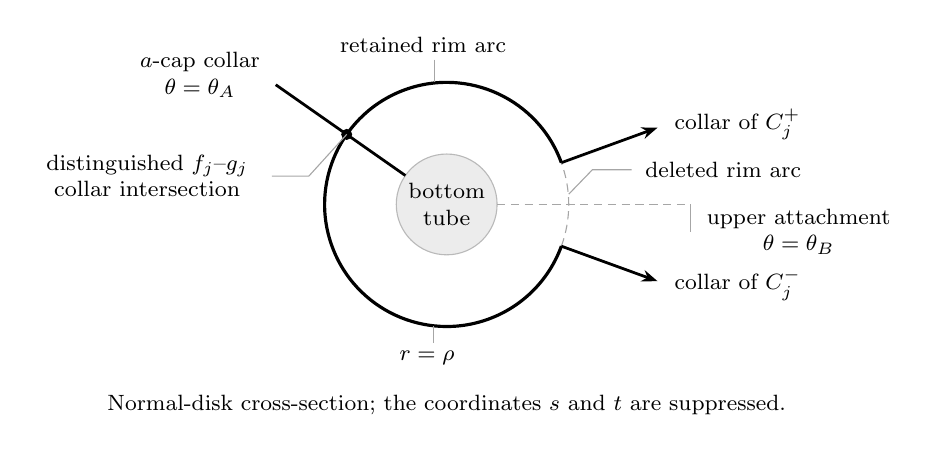
\begin{tikzpicture}[x=1cm,y=1cm,
 every node/.style={font=\small},
 collar/.style={line width=1pt},
 guide/.style={gray!70,densely dashed},
 annotation/.style={font=\footnotesize,align=center}]
 \fill[gray!15] (0,0) circle (0.64);
 \draw[gray!55] (0,0) circle (0.64);
 \node[annotation,text width=1.2cm] at (0,0)
  {bottom\\tube};

 \draw[line width=1.15pt] (20:1.55)
  arc[start angle=20,end angle=340,radius=1.55];
 \draw[guide] (340:1.55)
  arc[start angle=340,end angle=380,radius=1.55];
 \node[annotation] at (-0.3,2.03) {retained rim arc};
 \draw[gray!70] (-0.15,1.84)--(-0.15,1.55);
 \node[annotation] at (-0.25,-1.95) {\(r=\rho\)};
 \draw[gray!70] (-0.17,-1.76)--(-0.17,-1.54);

 \draw[collar] (145:0.64)--(145:2.65);
 \node[annotation,anchor=east] at (-2.25,1.64)
  {\(a\)-cap collar\\\(\theta=\theta_A\)};
 \fill (145:1.55) circle (2pt);
 \draw[gray!70] (-2.22,0.36)--(-1.75,0.36)--(145:1.55);
 \node[annotation,anchor=east,text width=2.8cm] at (-2.28,0.36)
  {distinguished \(f_j\)--\(g_j\)\\collar intersection};

 \draw[guide] (0.64,0)--(3.1,0);
 \draw[gray!70] (3.1,0)--(3.1,-0.35);
 \node[annotation,anchor=west] at (3.18,-0.35)
  {upper attachment\\\(\theta=\theta_B\)};
 \draw[collar,-{Stealth[length=2mm]}] (20:1.55)--(20:2.85);
 \draw[collar,-{Stealth[length=2mm]}] (340:1.55)--(340:2.85);
 \node[annotation,anchor=west] at (2.77,1.02)
  {collar of \(C_j^+\)};
 \node[annotation,anchor=west] at (2.77,-1.02)
  {collar of \(C_j^-\)};
 \draw[gray!70] (1.55,0.13)--(1.85,0.44)--(2.35,0.44);
 \node[annotation,anchor=west] at (2.40,0.44) {deleted rim arc};

 \node[annotation] at (0,-2.55)
  {Normal-disk cross-section; the coordinates \(s\) and \(t\) are suppressed.};
\end{tikzpicture}
\caption{The collar of the compressed rim sphere near the crossing of
\(a_j\) and \(b_j\) on the bottom surface. Restoring the coordinate
\(s\) along \(b_j\) turns the solid rim arc into the retained annulus,
the dashed rim arc near \(\theta_B\) into the removed compression band,
and the two outgoing segments into collars of the compression disks.
The marked point locates the distinguished collar intersection of
\(f_j\) with \(g_j\); the suppressed transverse surface coordinate is
\(t\). Only local collar directions are shown. The interiors of
\(C_j^\pm\), the other caps, and their possible mutual intersections
are not depicted.}
\label{fig:geometry-rim-collar}
\end{figure}


We count all remaining intersections. They occur in cap--cap plumbing
charts, because the parent bodies and the collar pieces just described
are disjoint away from their prescribed attachments. Each occurrence of
a \(D_{y,j}\) sheet in \eqref{eq:compressed-rim-sphere} has two indices:
\(\varepsilon\in\{+1,-1\}\) specifies the copy of \(C_j\), and
\(\eta\in\{+1,-1\}\) specifies the cap sheet inside that copy.
Its orientation coefficient is \(\varepsilon\eta\); the two indices are
shown in Figure~\ref{fig:geometry-sheets}.
At a plumbing chart with coordinates \((u,v)\in D^2\times D^2\), these
sheets are small parallel coordinate disks \(v=v_{\varepsilon,\eta}\);
the opposite core sheets are \(u=u_{\varepsilon',\eta'}\).
For any fixed opposing sheet, their local intersection signs differ by
the factor \(\eta\).

Fix \(\varepsilon\). The two paths to the \(\eta\)-sheets have the same
stem from the rim torus to that copy of the upper body. Their difference
is, up to this common conjugation, the upper basis loop \(z_j\).
That loop bounds \(D_{z,j}\), together with its tip-annulus collar, in
\(E\). Indeed those upper caps were disjoint from all the bottom tubes;
intersections with other caps do not remove them from \(E\).
An infinitesimal normal turn around the upper body also bounds a normal
fibre disk in \(E\), since that body was not removed.
It follows that the two intersection labels in \(\pi_1E\) agree.
The paired contributions are therefore
\[
 \varepsilon\eta\, h+\varepsilon(-\eta)\,h=0
 \quad\text{in }\mathbb Z[\pi_1E].
\]
The potential winding around the \emph{bottom} normal circle distinguishes
the outer \(\varepsilon\)-copies. We never compare those copies in this
cancellation: \(\varepsilon\) is held fixed throughout.

\begin{figure}[tbp]
\centering
\begin{minipage}[c]{0.40\textwidth}
\centering
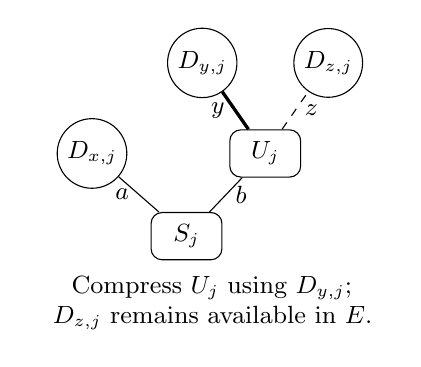
\begin{tikzpicture}[x=1cm,y=1cm,
 body/.style={draw,rounded corners,minimum width=9mm,minimum height=6mm},
 gropecap/.style={draw,circle,inner sep=2pt},
 every node/.style={font=\small}]
 \node[body] (s) at (0,0) {$S_j$};
 \node[gropecap] (a) at (-1.2,1.05) {$D_{x,j}$};
 \node[body] (u) at (1.0,1.05) {$U_j$};
 \node[gropecap] (y) at (0.2,2.2) {$D_{y,j}$};
 \node[gropecap] (z) at (1.8,2.2) {$D_{z,j}$};
 \draw (s)--node[left] {$a$}(a);
 \draw (s)--node[right] {$b$}(u);
 \draw[very thick] (u)--node[left] {$y$}(y);
 \draw[dashed] (u)--node[right] {$z$}(z);
 \node[align=center,text width=4.4cm] at (0.3,-0.85)
  {Compress \(U_j\) using \(D_{y,j}\);\\
   \(D_{z,j}\) remains available in \(E\).};
\end{tikzpicture}
\end{minipage}
\hfill
\begin{minipage}[c]{0.57\textwidth}
\centering
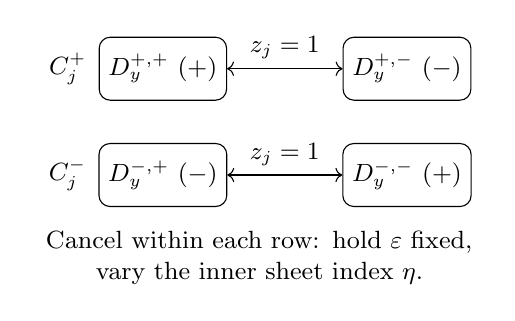
\begin{tikzpicture}[x=1cm,y=1cm,
 sheet/.style={draw,rounded corners,minimum width=1.45cm,minimum height=8mm},
 every node/.style={font=\small}]
 \node[sheet] (pp) at (0,1.1) {$D_y^{+,+}\ (+)$};
 \node[sheet] (pm) at (3.1,1.1) {$D_y^{+,-}\ (-)$};
 \node[sheet] (mp) at (0,-0.25) {$D_y^{-,+}\ (-)$};
 \node[sheet] (mm) at (3.1,-0.25) {$D_y^{-,-}\ (+)$};
 \draw[<->] (pp)--node[above] {$z_j=1$}(pm);
 \draw[<->] (mp)--node[above] {$z_j=1$}(mm);
 \node[anchor=east] at (-0.85,1.1) {$C_j^+$};
 \node[anchor=east] at (-0.85,-0.25) {$C_j^-$};
 \node[align=center,text width=5.6cm] at (1.2,-1.3)
  {Cancel within each row: hold \(\varepsilon\) fixed,\\
   vary the inner sheet index \(\eta\).};
\end{tikzpicture}
\end{minipage}
\caption{Combinatorial schematics, not projections of the four-dimensional
embedding. Left: the two-stage body and its one-sided upper contraction.
Right: the four occurrences of its surgery cap in the compressed rim
sphere; parentheses record their orientation coefficients
\(\varepsilon\eta\). The right panel suppresses the cap's subscript \(j\).
The labels \(z_j=1\) are equalities in \(\pi_1(E)\), proved using the upper
dual cap in \(E\).
No comparison between the two rows, which could involve a bottom
normal-circle meridian, is used.}
\label{fig:geometry-sheets}
\end{figure}


This accounts for every cap contribution to \(\lambda(f_i,g_j)\).
For \(g_i,g_j\), fix a sheet of \(g_i\) and the outer index of \(g_j\),
and cancel the inner index of \(g_j\) by the same argument. It also
applies when all parallel sheets at a plumbing point are counted
simultaneously. Hence the off-diagonal pairings of the \(g_j\) vanish.

The diagonal and framing admit a direct geometric check. The disk
\(C_j\) uses just the one core type \(D_{y,j}\), which has no self-plumbing.
That cap and its parallels are embedded and miss the parent body off their
attachments. Thus \(C_j\), and then the sphere in
\eqref{eq:compressed-rim-sphere}, can each be individually embedded.
Mutual intersections with other \(g_i\) do not affect this assertion.
The normal frame of the rim torus is
\((\partial_t,\partial_r)\). Along the outgoing radial compression collar
the cap normal frame is \((\partial_t,\partial_\theta)\).
Rounding the surgery corner rotates the second vector from
\(\partial_r\) to \(\partial_\theta\), while the first remains fixed.
The product framing matched in Lemma~\ref{lem:marked-body} extends this
ordered pair. The earlier compression \eqref{eq:one-sided-contraction}
is the same framed operation, so its outgoing \(b_j\)-annulus has exactly
the required inherited framing. Consequently \(g_j\) has trivial normal
bundle. Its normal push-off is disjoint from it, proving the diagonal
\(\lambda(g_j,g_j)=0\); its embedded representative also gives
\(\widetilde\mu(g_j)=0\).

Combining this with the distinguished collar point proves all the stated
equalities. Small perturbations make the finite collection generic while
preserving the calculation and the framings.
\end{proof}

Assumption~\ref{ass:disk}, applied to \(E\) and
Lemma~\ref{lem:exterior-duals}, now gives pairwise disjoint locally flat
embedded replacement caps with the specified boundary framings.
Compress each bottom \(S_j\) with two parallels of its replacement cap,
using the returning annuli in the removed tube. The result is a collection
of pairwise disjoint properly embedded disks in \(X\), bounded by the
initial grope boundaries. The framing is what makes this compression
locally flat with the required product collar. No relative homotopy of
the replacement cap to \(f_j\) is used. The output dual-sphere part of a
disk embedding theorem is not used either.

\subsection{Equivariant cuts with connected pieces}

The preceding compression uses the assumed replacement disks to make
the initial grope boundaries bound disjoint disks. We now keep those
disks in their prescribed vertex regions while cutting the ambient
plumbing into smooth pieces. Connectedness of these pieces will be
needed for the restriction maps in the final part of this section.

\begin{lemma}[Connected tree cuts]
\label{lem:connected-tree-cuts}
Suppose the initial grope boundaries bound the disjoint disks just
constructed. Then the boundary map to the plumbing tree extends
equivariantly to a map whose cuts can be chosen to have the connected
vertex and edge pieces asserted in
Proposition~\ref{prop:geometric-reduction}. Every lifted disk lies in
its prescribed vertex piece.
\end{lemma}

\begin{proof}
Lift the disks to \(\widetilde X\). Each is labelled by the vertex
containing its boundary. Distinct translates and distinct members have
disjoint images, because the disks were embedded and disjoint in \(X\).
Prescribe the map to be constant at the label vertex on a neighbourhood
of every such disk, and retain the fixed boundary map. These prescriptions
agree on their overlaps.

An equivariant extension is equivalently a section of the associated
bundle over \(X\) with fibre the tree. The prescribed section extends first
to a neighbourhood of the prescribed closed set, since the tree is an
absolute neighbourhood retract, and then over the remaining cells,
since the fibre is contractible. One may take a finite triangulation of
the smooth ambient manifold for the latter extension after shrinking the
neighbourhood. The section formulation ensures equivariance. This step
does not require extending to the noncontractible quotient graph by
contractibility of that graph.

On the quotient, approximate the map smoothly over the open middle
intervals of its finitely many graph edges, keeping it fixed on the
specified boundary collars and away from the disk neighbourhoods.
Choose regular values there. Their inverse images are compact smooth
proper hypersurfaces, disjoint from all disks. After rescaling an edge
interval we call its chosen value the midpoint. The lift of the level
corresponding to a tree edge \(e\) has exactly one boundary component:
the specified torus \(T_e\). More precisely, the unique component meeting
the boundary contains that torus as its entire boundary; every other
component of that level is closed.

Consider the component graph \(\mathcal T'\) of this cut in
\(\widetilde X\): its vertices are connected complementary pieces, and
its edges are connected cut hypersurfaces. It is connected. The collapse
to \(\mathcal T'\) is surjective on fundamental groups: a finite graph
loop is realised by choosing crossing points and joining successive
points by paths in the connected pieces. By
\eqref{eq:plumbing-homotopy}, the fundamental group of \(\widetilde X\)
is generated by the extra loops in its boundary pieces, with whiskers.
Each such loop maps to a vertex of \(\mathcal T'\). Thus
\(\pi_1\mathcal T'=0\), and \(\mathcal T'\) is a tree.

The boundary pieces and their torus collars determine a principal copy
\(\mathcal T\) of the original tree inside \(\mathcal T'\).
To check injectivity directly, remove the chosen midpoints from the
target tree. A connected component of their inverse-image complement
maps into just one resulting vertex-star component. It cannot contain
both \(K_v\) and \(K_w\) for \(v\ne w\). Similarly distinct principal
edge components have distinct midpoint labels. The boundary collars
give exactly the required incidences. Hence the principal copy is
indeed an embedded subtree.

Every remaining branch of \(\mathcal T'\) has a unique nearest vertex in
\(\mathcal T\). A deck transformation stabilising a vertex or edge of
such a branch fixes that nearest principal vertex and is therefore the
identity. Thus all these stabilisers are trivial. The finite compact
quotient cut has only finitely many components, so \(\mathcal T'\)
has finite quotient. Trivial stabilisers imply finite valence.
Moreover distance to \(\mathcal T\) is invariant under translation and
is bounded on the finite set of component orbits. A finite-valence tree
of bounded depth rooted at one principal vertex is finite.

Ignore the closed cuts in each such finite hanging branch, merging it
with its principal vertex piece. This operation is equivariant, preserves
compact quotient and the principal hypersurfaces, and gives connected
vertex pieces \(V_v\) and a single connected edge piece \(Y_e\) with
\(\partial Y_e=T_e\). All prescribed disks remain in their own pieces:
they lay in the component containing their boundary before the merging.
The \(Y_e\) and \(V_v\) are smooth manifolds with corners; the topological
disks themselves were never required to become smooth.
\end{proof}

Each initial boundary is therefore null-homotopic in its vertex piece.
Its actual boundary word has the three-slot properties
\eqref{eq:grope-word-properties} with inputs
\eqref{eq:three-slot-inputs}. This proves precisely the relation statement
in Proposition~\ref{prop:geometric-reduction}.

\subsection{The parity quotient and its peripheral homology}

Send every plumbing generator of \(F_m\) to \(1\in\mathbb Z/2\).
The quotient of \(\widetilde X\) by the kernel has two principal vertex
pieces \(A,B\) and two lifts of each of the \(m\) plumbing edges.
Thus there are \(2m\) edges. The free translation interchanging parity
gives a deck involution interchanging \(A\) and \(B\), and pairing these
edge lifts. Equation~\eqref{eq:plumbing-homotopy}, or the same
contractible-overlap argument in this quotient, gives
\begin{equation}
\label{eq:parity-homotopy}
 X_2\simeq\Gamma\ \text{with \(p\) extra circles at each vertex},
 \qquad
 |V\Gamma|=2,\quad |E\Gamma|=2m.
\end{equation}
In particular \(H^q(X_2;k)=0\) for \(q\geq2\), and
\(\dim_kH^1(X_2;k)=2m-1+2p\).
The extra loops at the two vertices can be assigned independently in
the free ambient fundamental group. All port meridians are trivial
there, since they bound the corresponding handle-core disks in \(X_2\).

\begin{lemma}[Restriction maps and coordinate slopes]
\label{lem:geometric-edge-cohomology}
The cohomology and slope conclusions of
Proposition~\ref{prop:geometric-reduction} hold.
For each edge piece one also has
\begin{equation}
\label{eq:edge-relative-cohomology}
 H^1(Y_i,\partial Y_i;k)
  \cong\ker\bigl(H^1(Y_i;k)\longrightarrow H^1(\partial Y_i;k)\bigr),
 \qquad b_2(Y_i)=b_1(Y_i)-1.
\end{equation}
\end{lemma}

\begin{proof}
Insert small edge collars so that Mayer--Vietoris applies to the two
vertex pieces with intersection the disjoint union of the \(Y_i\).
Its degree-one portion is
\[
\begin{aligned}
 H^0(A;k)\oplus H^0(B;k)
 &\longrightarrow\bigoplus_iH^0(Y_i;k)
 \longrightarrow H^1(X_2;k)\\
 &\longrightarrow H^1(A;k)\oplus H^1(B;k)
 \xrightarrow{\,R\,}\bigoplus_iH^1(Y_i;k)
 \longrightarrow0 .
\end{aligned}
\]
Connectedness makes the first cokernel have dimension \(2m-1\);
these are the graph classes of \(\Gamma\).
They restrict to zero on the vertex pieces. The remaining kernel of
\(R\) has dimension \(2p\). Evaluation on the \(p\) extra loops at each
vertex identifies this kernel with \(k^{2p}\): their ambient classes in
\eqref{eq:parity-homotopy} give surjectivity, and an ambient class with
zero extra evaluations is a graph class and restricts to zero.
Consequently \(R\) restricts to an isomorphism on the kernel of the
extra evaluations. The next part of the same sequence, using
\(H^2(X_2;k)=H^3(X_2;k)=0\), gives
\eqref{eq:geometry-mv-degree-two}.

Let \(Y\) be one of the connected oriented three-manifolds with single
torus boundary \(T\). Poincaré--Lefschetz duality and
\(\chi(Y)=\chi(T)/2=0\) give \(b_2(Y)=b_1(Y)-1\).
The exact sequence of the pair, using connectedness of \(Y,T\), gives
the isomorphism in \eqref{eq:edge-relative-cohomology}.
Equivalently the image of \(H_1(T;k)\) in \(H_1(Y;k)\) has dimension
one, the half-lives/half-dies statement.

Write \(u,v\) for the original two coordinate directions on \(T\).
One is a longitude in the boundary piece on one side and the other
is a longitude on the other side. Suppose both had nonzero image in
the one-dimensional image in \(H_1(Y;k)\). They would then be nonzero
scalar multiples of each other. A cohomology class restricted from
the first side annihilates its longitude and hence both directions;
the same is true of a class restricted from the second side.
Surjectivity of \(R\) would imply that every class of \(H^1(Y;k)\)
annihilates both directions, contradicting the one-dimensional image.
Thus one original coordinate direction has zero image and the other
has nonzero image. Denote them by \(\beta,\alpha\), respectively.
In cohomology the boundary restriction image is the line spanned by
the coordinate form dual to \(\alpha\).

The deck involution preserves the transported slope choice and swaps the
two vertices. For the two lifts of each plumbing edge it therefore
interchanges which one has its plus endpoint at \(A\).
Exactly one lift in each pair is active, giving exactly \(m\) active
edges. At \(A\) their \(\alpha\)'s are distinct port meridians, and at
\(B\) their \(\beta\)'s are distinct port meridians. Their three-slot
relations, with every independent choice of the stipulated conjugators,
were all included before any slope was selected.
\end{proof}

\begin{proof}[Proof of Proposition~\ref{prop:geometric-reduction}]
The plumbing construction supplies \(X\), its boundary pieces, and its
regular cover. Lemma~\ref{lem:marked-body} supplies the finite marked
family. Lemma~\ref{lem:exterior-duals} checks every input hypothesis of
Assumption~\ref{ass:disk} in the exterior of the bottoms.
The replacement disks and framed bottom compressions then give the
disks required by Lemma~\ref{lem:connected-tree-cuts}, and hence the
relations in connected vertex pieces. Finally
Lemma~\ref{lem:geometric-edge-cohomology} gives the claimed parity-quotient data.
\end{proof}

\section{A finite tensor obstruction}\label{sec:tensor}

This section proves an algebraic obstruction to the formal data that will
arise from the two vertex pieces.  The formal parametrizations may involve
every edge block; each potential depends only on its own block.
All parameter rings below retain every mixed square-free parameter monomial.

For a characteristic-zero field \(K\), write \(K\langle h\rangle\) for the
ring of algebraic power series at the origin, identified with the
henselization of \(K[h]_{(h)}\) inside \(K[[h]]\).  An algebraic germ can
therefore be represented by a regular function on a pointed étale
neighborhood.  Gradients in this section always differentiate internal
coordinates, keeping the external parameters fixed.

\begin{theorem}[Finite tensor obstruction]\label{thm:tensor-obstruction}
Let \(h=(h_1,\ldots,h_n)\) be a finite list of coordinate blocks over a
characteristic-zero field \(K\), of total dimension \(N\).  Let
\(I\subset\{1,\ldots,n\}\) have cardinality \(m\geq5\), and let
\[
 F_i\in K\langle h_i\rangle\quad(1\leq i\leq n),
 \qquad b_i\in K\langle h_i\rangle\quad(i\in I).
\]
Put
\[
 T=K[t_i:i\in I]/(t_i^2:i\in I),\qquad
 S_0(h)=\sum_{i=1}^nF_i(h_i),\qquad
 S_t(h)=S_0(h)+\sum_{i\in I}t_i b_i(h_i).
\]
Suppose there are formal parametrizations
\[
 H_L(x,t)\in (x,t)\,T[[x]]^N,\qquad
 H_R(y)\in (y)\,K[[y]]^N,
\]
where \(x\) has \(a\) coordinates and \(y\) has \(N-a\) coordinates, with
the following properties.
\begin{enumerate}[label=\textup{(\roman*)}]
 \item The central tangent maps
 \[
  \partial_xH_L(0,0):K^a\longrightarrow K^N,\qquad
  \partial_yH_R(0):K^{N-a}\longrightarrow K^N
 \]
 are injective and have complementary images.
 \item The identities
 \[
     S_t(H_L(x,t))=0,\qquad S_0(H_R(y))=0
 \]
 hold in \(T[[x]]\) and \(K[[y]]\), respectively.
 \item For every three distinct \(i,j,k\in I\),
 \begin{align}
 t_i t_j t_k
 &\in\bigl((\partial_{h_\nu}S_t)(H_L(x,t)):
                    1\leq\nu\leq N\bigr)\subset T[[x]],
       \label{eq:tensor-source-membership}\\
 (b_i b_j b_k)(H_R(y))
 &\in\bigl((\partial_{h_\nu}S_0)(H_R(y)):
                    1\leq\nu\leq N\bigr)\subset K[[y]].
       \label{eq:tensor-target-membership}
 \end{align}
\end{enumerate}
Then these data do not exist.
\end{theorem}

Condition (i) makes the parametrizations smooth formal graph embeddings,
including over the full ring \(T\).  Nilpotent constant displacements of
\(H_L\) are allowed.  The ideals in
\eqref{eq:tensor-source-membership}--\eqref{eq:tensor-target-membership}
are the actual gradient ideals; no passage to their radicals is made.
There is no flatness assumption on their quotients.

The later construction supplies the hypotheses as follows; all triples
in the table have distinct active indices.
\begin{center}
\begin{tabular}{@{}
 >{\raggedright\arraybackslash}p{0.25\linewidth}
 >{\raggedright\arraybackslash}p{0.30\linewidth}
 >{\raggedright\arraybackslash}p{\dimexpr0.45\linewidth-4\tabcolsep\relax}
 @{}}
\toprule
Input & Source of the data & Later verification \\
\midrule
Separate algebraic \(F_i(h_i)\) and \(b_i(h_i)\)
 & Individual marked edge models and polynomial perturbations
 & Theorem~\ref{thm:edge-algebraicity} and
   Section~\ref{subsec:vertex-polynomial} \\[4pt]
Complementary central tangents
 & Restriction maps after fixing the prescribed evaluations
 & Lemma~\ref{lem:vertex-linear} \\[4pt]
Exact vanishing \(S_t|_L=0\) and \(S_0|_R=0\)
 & Stokes and section corrections preserving the residual quotient
 & Lemmas~\ref{lem:vertex-offshell-identities},
   \ref{lem:vertex-correction}, and
   \ref{lem:tensor-nilpotent-correction} \\[4pt]
Every source triple \(t_i t_j t_k\) in the restricted gradient ideal on \(L\)
 & Boundary laws at \(A\)
 & Lemma~\ref{lem:vertex-triple-ideals} \\[4pt]
Every target triple \(b_i b_j b_k\) in the restricted gradient ideal on \(R\)
 & Boundary laws at \(B\) and polynomial holonomy weights
 & Lemma~\ref{lem:vertex-triple-ideals} and
   Section~\ref{subsec:vertex-polynomial} \\
\bottomrule
\end{tabular}
\end{center}

The threshold \(m\geq5\) comes from two counts.  The target triple
identities put the right graph's Koszul class in a sum of tensor patterns
with at most two active factors outside the multiplication kernels.
A compatible projection for the induced exterior differential then gives
pure tensors of classes with at least \(m-2\geq3\) active factors both
closed for that differential and killed by \(b_i\).
These give three independent parameter lifts, and the source triple
membership forces their pairing to vanish.  The closure statements concern
Koszul classes; the chosen form representatives need not be closed for
ordinary \(\dd\).

\subsection{Algebraic approximation and finite specialization}

\begin{lemma}\label{lem:tensor-reduction}
If the data in Theorem~\ref{thm:tensor-obstruction} existed, data satisfying
the same conditions would exist over a field of positive characteristic
\(p\), for arbitrarily large \(p\).  The edge functions would still be
separated in their original blocks.
\end{lemma}

\begin{proof}
First put the parametrizations into graph form.  Choose complementary
linear projections adapted to their central tangent spaces.  For \(L\),
the chosen projection of \(H_L\) has invertible \(x\)-Jacobian modulo
\((x,t)\).  It therefore has a formal inverse over \(T\), with the parameters
fixed.  Its constant displacement is in \((t)\), so this is a legitimate
substitution in the complete local ring \(T[[x]]\).
For \(R\) the same assertion is the ordinary formal inverse function
theorem.  After these reparametrizations each graph has a fixed linear
projection equal to its independent variables.

We describe explicitly the approximation problem for \(L\).
For \(A\subset I\), let \(t_A=\prod_{i\in A}t_i\), including \(t_\varnothing=1\).
Expand its graph functions and all the coefficients witnessing
\eqref{eq:tensor-source-membership} in this finite basis:
\[
 H_L(x,t)=\sum_{A\subset I}t_A H_A(x),\qquad
 c(x,t)=\sum_{A\subset I}t_A c_A(x).
\]
All unknown coefficient functions have the same list \(x\) of independent
variables.

The fixed algebraic functions \(F_i,b_i\) admit finite pointed étale
presentations.  In such a presentation, differentiation in \(h_\nu\)
extends uniquely from the polynomial coordinate ring: implicit
differentiation expresses the derivative of every represented function
using the inverse étale Jacobian.  Thus the functions and their ambient
first derivatives can be handled in one finite presentation.  Introduce
auxiliary unknowns for its coordinates and its inverse units, and expand
them too in the basis \(t_A\).  Equating coefficients in the following
identities gives a finite polynomial system:
\begin{itemize}
 \item the étale presentation equations and the inverse-unit equations;
 \item the fixed graph-projection equation;
 \item \(S_t(H_L)=0\);
 \item each equation expressing \(t_i t_j t_k\) as a linear combination
       of the restricted ambient gradient entries.
\end{itemize}
No derivative of an unknown graph function occurs.  The only derivatives
are the fixed ambient derivatives of the given potentials, represented
as just described.  The existing formal graph and membership witnesses
give a formal solution of this polynomial system.

Artin approximation over the henselization \(K[x]_{(x)}^h\)
\cite[Theorem~1.10]{Artin1969} supplies an algebraic solution preserving
the desired finite jets.  Preserve the centers, the branch centers of
the étale presentations, and the central first graph jet.
Do the same independently for \(R\), encoding
\eqref{eq:tensor-target-membership} in its own independent variables \(y\).
These two systems share only fixed functions.  Their compatibility
condition is the open condition of complementary central tangents, which
the preserved jets retain.  There is consequently no nested approximation
problem.  If one independent-variable list is empty, the corresponding
system is already a finite system over \(K\).

We now have finitely many algebraic functions and finitely many exact
identities in henselizations.  Each function is represented on a finite
pointed étale neighborhood.  An identity in a henselization holds at some
finite stage of the filtered system of these neighborhoods.  Enlarging
the stages finitely many times represents all the functions, compositions,
membership identities, branch centers, and inverse units together.
Their finite presentations descend to a finitely generated integral
\(\mathbb Z\)-subalgebra \(A\subset K\), after adjoining the required
inverse units.  In particular we retain invertibility of the étale
Jacobians and of the transverse tangent determinant.  The implicit
differentiation formulas descend as well, so the specialized gradient
entries remain the derivatives of the specialized potentials.
The original presentations for the edge functions involve only their
own blocks \(h_i\), and retain that property after descent.

For completeness, this finite localization still has closed points in
arbitrarily large positive characteristics.  The nonzero finite-type
\(\mathbb Q\)-algebra \(A\otimes_{\mathbb Z}\mathbb Q\) has a maximal
ideal with residue field a number field \(E\).  The images of the finitely
many generators of \(A\), including all inverted elements, belong to
\(\mathcal O_E[1/d]\) for some positive integer \(d\).
Reduction at any prime of \(\mathcal O_E\) over a rational prime not
dividing \(d\) gives a homomorphism from \(A\) to a finite field.
All the declared units remain units.  The reduced pointed étale
presentations give formal germs over that residue field, satisfying the
same identities and the same tangent condition.
\end{proof}

\begin{remark}\label{rem:tensor-coefficient-field}
The lemma also applies when \(K=\mathbb C((\sigma))\).
Only finitely many elements of \(K\) occur as coefficients of the finite
presentations, and each is treated as a single coefficient.
Specialization is performed on \(A\), not coefficientwise on Laurent
series or on the whole field \(K\).
In particular, no boundedness of the negative \(\sigma\)-orders of the
coefficients of an Artin solution is required.
The algebraicity of the fixed separated potentials is essential:
the argument does not assert that ordinary Artin approximation can
algebraize arbitrary unknown formal potentials while preserving separate
variable restrictions.
\end{remark}

\subsection{Truncated forms and transverse graph classes}

The approximation step preserves all graph identities and actual ideal
memberships. We now turn their positive-characteristic specializations
into identities in finite-dimensional complexes, where transverse
graphs can be tested by a nonzero pairing.

Fix a specialization supplied by Lemma~\ref{lem:tensor-reduction} in
characteristic \(p>2\), and denote its field by \(\kk\).
Continue to use the same letters for the specialized germs.
Write \(z_1,\ldots,z_N\) for all internal coordinates and set
\[
 A_p=\kk[z_1,\ldots,z_N]/(z_1^p,\ldots,z_N^p),\qquad
 \Omega_p=A_p\otimes_\kk\bigwedge\nolimits_\kk
                   \langle \dd z_1,\ldots,\dd z_N\rangle .
\]
This is the ordinary algebra of differential forms of \(A_p\).
Its differential is well defined because \(\dd(z_\nu^p)=0\).
With external parameters, use
\[
 T_p=\kk[t_i:i\in I]/(t_i^2:i\in I),
 \qquad \Omega_{p,T}=\Omega_p\otimes_\kk T_p,
\]
and differentiate only in the internal coordinates.
All these spaces are finite over the indicated coefficient rings.

\begin{lemma}\label{lem:tensor-frobenius}
Every formal change of internal coordinates over \(T_p\) that is centered
modulo \((t)\) preserves the ideal
\((z_1^p,\ldots,z_N^p)\).  Hence it induces an automorphism of the truncated
algebra and of its relative differential forms.
\end{lemma}

\begin{proof}
If \(c\in(z,t)T_p[[z]]\), Frobenius shows that \(c^p\) belongs to
\((z_1^p,\ldots,z_N^p)\): every nonconstant internal monomial acquires an
exponent divisible by \(p\), and every positive parameter monomial has
zero \(p\)-th power.  Apply this to each new coordinate.
The inverse coordinate change has the same property, giving equality of
the ideals and the asserted automorphisms.
\end{proof}

Define a \(\kk\)-linear functional on forms, zero outside exterior degree
\(N\), by
\[
 \int f(z)\,\dd z_1\wedge\cdots\wedge\dd z_N
   =[z_1^{p-1}\cdots z_N^{p-1}]f .
\]
Extend it \(T_p\)-linearly in the presence of parameters.
It vanishes on exact forms: a derivative contributing exponent \(p-1\)
in its differentiated variable would have to come from exponent \(p\),
whose derivative is zero.  Consequently, for homogeneous forms,
\begin{equation}\label{eq:tensor-integration-by-parts}
 \int\dd\alpha\wedge\beta
       =-(-1)^{|\alpha|}\int\alpha\wedge\dd\beta .
\end{equation}

Let \(c_1,\ldots,c_r\) be graph equations for a smooth formal graph over
the parameter ring.  Their joint center is zero modulo \((t)\).
Its graph form is
\begin{equation}\label{eq:tensor-thom-form}
 U_c=\bigl(c_1^{p-1}\dd c_1\bigr)\wedge\cdots\wedge
                       \bigl(c_r^{p-1}\dd c_r\bigr)
       \in\Omega_{p,T}^{r}.
\end{equation}
This expression involves only a finite jet after truncation.

\begin{lemma}\label{lem:tensor-graph-form}
The form \(U_c\) is \(\dd\)-closed and is annihilated by the graph ideal.
Every internal one-form whose restriction to the graph is zero wedges
to zero with \(U_c\).
For two central graphs with complementary tangents and graph forms
\(U_0,V\),
\begin{equation}\label{eq:tensor-nonzero-pairing}
                     \int U_0\wedge V\ne0 .
\end{equation}
\end{lemma}

\begin{proof}
Each factor \(c_j^{p-1}\dd c_j\) is closed, and \(c_j^p=0\) in the
truncated ring by Lemma~\ref{lem:tensor-frobenius}.
This proves the first two assertions.
In graph coordinates, the kernel of restriction of internal one-forms is
the sum of graph-ideal multiples of one-forms and the span of the
\(\dd c_j\).  Both summands wedge to zero with \(U_c\).
This description remains valid after truncation because the graph
coordinate change preserves the truncation ideal.

For the pairing, concatenate the central graph equations for the two
graphs, and let \(M\) be their linear coefficient matrix in the original
coordinates.  Complementarity says that \(M\) is invertible.
The coefficient part of \(U_0\wedge V\) has degree at least \(N(p-1)\);
all terms of higher degree vanish in \(A_p\).
Thus only the linear terms of the graph equations and the constant terms
of their differentials contribute.  A linear coordinate change \(M\)
acts on the polynomial socle
\(\kk z_1^{p-1}\cdots z_N^{p-1}\) by \(\det(M)^{p-1}\), and on the
exterior top form by \(\det(M)\).  To check the socle assertion one may
use diagonal matrices, permutations, and elementary transvections:
for a transvection every nonconstant binomial term has an exponent at
least \(p\) and vanishes.  These matrices generate the general linear
group.  The pairing is therefore \(\det(M)^p\), up to the choice of order
of the graph equations, and is nonzero.
\end{proof}

Let \(U_t\) be the graph form for \(L\), and let \(V\) be the graph form
for \(R\).  Define the degree-one operators
\[
       D_t=\dd S_t\wedge(-),\qquad D=\dd S_0\wedge(-).
\]
Both square to zero.  The graph identities and
Lemma~\ref{lem:tensor-graph-form} give
\begin{equation}\label{eq:tensor-graph-cycles}
 D_tU_t=0,\qquad DV=0,\qquad
 \dd U_t=0,\qquad\dd V=0 .
\end{equation}
In particular \(DU_0=0\) and the nonzero pairing
\eqref{eq:tensor-nonzero-pairing} is defined.

\begin{lemma}\label{lem:tensor-membership-boundary}
For every three distinct active indices \(i,j,k\), there are actual forms
\(B_{ijk}\) and \(C_{ijk}\) with
\begin{equation}\label{eq:tensor-actual-boundaries}
 t_i t_j t_k U_t=D_t B_{ijk},\qquad
 b_i b_j b_k V=D C_{ijk}.
\end{equation}
The first equality is over the full parameter algebra \(T_p\).
\end{lemma}

\begin{proof}
Lift the graph membership coefficients to the ambient ring.
The difference between the asserted scalar and the resulting ambient
gradient combination belongs to the graph ideal, so it annihilates the
graph form.  If \(\iota_\nu\) is contraction with the coordinate vector
\(\partial/\partial z_\nu\), then
\[
 \iota_\nu D_t+D_t\iota_\nu
                =(\partial_{z_\nu}S_t)\,\id.
\]
For a \(D_t\)-cycle \(U_t\), multiplication by
\(\sum_\nu a_\nu\partial_{z_\nu}S_t\) is consequently
\[
 \left(\sum_\nu a_\nu\partial_{z_\nu}S_t\right)U_t
       =D_t\left(\sum_\nu a_\nu\iota_\nu U_t\right).
\]
The operator \(D_t\) does not differentiate the coefficients \(a_\nu\).
This proves the first equality, and the same argument with \(D,V\)
proves the second.
\end{proof}

We will use two elementary facts about this pairing.  If
\(\theta\) is a one-form and \(D_\theta=\theta\wedge(-)\), then, for
homogeneous \(\alpha\),
\begin{equation}\label{eq:tensor-wedge-adjoint}
 (D_\theta\alpha)\wedge\beta
          =(-1)^{|\alpha|}\alpha\wedge D_\theta\beta.
\end{equation}
Thus a \(D_\theta\)-boundary wedges to zero with a
\(D_\theta\)-cycle, even before integration.
Also \(\dd D+D\dd=0\), since \(\dd^2S_0=0\).
Ordinary differentiation therefore induces a differential on the
homology of \(D\); Equation~\eqref{eq:tensor-integration-by-parts}
continues to test its boundaries against actual closed representatives.

\subsection{Two homologies and a compatible projection}

We have graph cycles with a nonzero pairing and actual boundary
identities for every triple. The separate edge blocks now let us
analyze the target graph class one factor at a time. We first take
Koszul homology, then use the differential induced on it by ordinary
exterior differentiation.

Let \(\Omega_i\) be the truncated form algebra in the block \(h_i\), and
write
\[
 D_i=\dd F_i\wedge(-),\qquad H_i=H(\Omega_i,D_i).
\]
The tensor products of graded spaces and operators in what follows use
the usual Koszul signs.  The block separation gives
\[
 (\Omega_p,D)=\bigotimes_{i=1}^n(\Omega_i,D_i),\qquad
 H(\Omega_p,D)=\bigotimes_{i=1}^n H_i .
\]
The second equality is the finite-dimensional Künneth isomorphism over
the field \(\kk\).
Let \(\delta_i\) denote the differential induced on \(H_i\) by ordinary
\(\dd\), and let \(\delta\) be their tensor differential.
For \(i\in I\), multiplication by \(b_i\) induces a degree-zero
endomorphism \(B_i\) of \(H_i\), since it commutes with \(D_i\).
Set
\[
                         K_i=\ker B_i .
\]
There is no assertion that \(K_i\) is a \(\delta_i\)-subcomplex.

\begin{lemma}[Kernel support]\label{lem:tensor-kernel-support}
Let \(v\in\bigotimes_{i=1}^nH_i\) be killed by
\(B_iB_jB_k\) for every three distinct active indices.
Then \(v\) belongs to the sum of tensor subspaces having all but at most
two active factors in the corresponding \(K_i\).
\end{lemma}

\begin{proof}
Choose a graded complement \(J_i\) to \(K_i\) in each active factor.
The restriction of \(B_i\) to \(J_i\) is injective.
For a fixed triple, the kernel of its tensor operator is the sum of
subspaces having a \(K_i\) factor in at least one of the three specified
positions: the induced tensor of injections on the quotient by those
kernels is injective.
Expand the whole tensor product using \(H_i=K_i\oplus J_i\).
Intersecting the kernel conditions for all triples leaves exactly the
summands with at most two active \(J_i\) positions.
\end{proof}

\begin{lemma}[Projection preserving kernel representatives]
\label{lem:tensor-kernel-projection}
Let \((H,\delta)\) be a finite-dimensional graded complex over a field,
and let \(K\subset H\) be any graded subspace.
There is a chain projection \(P:H\to H\), homotopic to the identity,
whose image is a space of representatives for \(H(H,\delta)\) and which
satisfies
\[
                    P(K)\subset K\cap\ker\delta .
\]
\end{lemma}

\begin{proof}
Write \(Z=\ker\delta\) and \(B=\im\delta\).
Choose a complement \(A_K\) to \(K\cap B\) in \(K\cap Z\), and extend
\(A_K\) to a complement \(A\) to \(B\) in \(Z\).
Choose a complement \(W_K\) to \(K\cap Z\) in \(K\).
It is disjoint from \(Z\), so extend it to a complement \(W\) to \(Z\)
in \(H\).  All these choices are made degree by degree.
Then
\[
                       H=B\oplus A\oplus W .
\]
Let \(P\) be projection onto \(A\).  It is a chain map, and
\(P(K)\subset A_K\subset K\cap Z\).
The map \(\delta:W\to B\) is an isomorphism with the appropriate shift
of degrees.  Define a degree-minus-one map \(s\) to be its inverse on
\(B\), and zero on \(A\oplus W\).  Then
\[
                        \id-P=\delta s+s\delta .
\]
\end{proof}

Apply Lemma~\ref{lem:tensor-kernel-projection} to each active factor
\((H_i,\delta_i,K_i)\), and choose an ordinary homology projection in
each inactive factor.  Denote these maps by \(P_i\), and put
\(\Pi=\bigotimes_iP_i\).  This tensor projection is chain-homotopic
to the identity.  Indeed, the telescoping identity for
\(\id-\bigotimes_iP_i\), together with the individual homotopies and
the graded tensor convention, supplies a homotopy for the total
differential \(\delta\).

Let \(v=[V]\in H(\Omega_p,D)\).  Equations
\eqref{eq:tensor-actual-boundaries} imply the hypotheses of
Lemma~\ref{lem:tensor-kernel-support}, and \(\delta v=0\) by
\eqref{eq:tensor-graph-cycles}.  Thus \(\Pi v\) is a sum of homogeneous
pure tensors
\begin{equation}\label{eq:tensor-pure-cycles}
                   v_1\otimes\cdots\otimes v_n
\end{equation}
such that every \(v_i\) is a \(\delta_i\)-cycle and at least \(m-2\)
active factors lie in \(K_i\cap\ker\delta_i\).
This conclusion follows by applying \(\Pi\) to the tensor subspaces in
Lemma~\ref{lem:tensor-kernel-support}; the projection of a kernel factor
is still a kernel factor.
Since \(m\geq5\), every nonzero pure tensor in this sum has at least three
such active factors.

Choose \(D_i\)-cycle representatives for all the factors in
\eqref{eq:tensor-pure-cycles}, and let \(V'\) be the resulting sum of
actual forms.  The chain homotopy for \(\Pi\) shows that
\([V']-[V]=\delta[Z]\) for some class in \(H(\Omega_p,D)\).
Choose a \(D\)-cycle representative \(Z\).
There is then an actual form \(E\) such that
\begin{equation}\label{eq:tensor-chain-replacement}
                         V'-V=\dd Z+D E .
\end{equation}
Pairing with \(U_0\), equations
\eqref{eq:tensor-integration-by-parts},
\eqref{eq:tensor-graph-cycles}, and
\eqref{eq:tensor-wedge-adjoint} give
\begin{equation}\label{eq:tensor-pairing-preserved}
                    \int U_0\wedge V'=\int U_0\wedge V .
\end{equation}
The representatives composing \(V'\) need not be closed for ordinary
\(\dd\).  Their classes are \(\delta_i\)-cycles, which is precisely what
was used to obtain \eqref{eq:tensor-chain-replacement}.

\subsection{Lifts over a three-parameter cube}

The replacement class has the same pairing with the source graph as
the original target class. Each of its tensor summands has at least
three active factors lying in both the multiplication kernel and the
kernel of the induced differential. Those three factors supply the
parameter lifts used to force that summand's pairing to vanish.

\begin{proof}[Proof of Theorem~\ref{thm:tensor-obstruction}]
Suppose the stated data exist and perform the reduction and constructions
above.  Consider one pure tensor \eqref{eq:tensor-pure-cycles} contributing
to \(V'\).  Choose three active positions \(i,j,k\) in which
\[
                   B_\nu v_\nu=0,\qquad\delta_\nu v_\nu=0 .
\]
On \(H_\nu\), the commutator identity is
\[
       [\delta_\nu,B_\nu]
         =\delta_\nu B_\nu-B_\nu\delta_\nu
         =[\,\dd b_\nu\wedge(-)\,].
\]
It follows that \([\,\dd b_\nu\wedge(-)\,]v_\nu=0\).
For a homogeneous \(D_\nu\)-cycle representative \(a_\nu\) of \(v_\nu\),
there is therefore a form \(w_\nu\) of the same exterior degree with
\[
                    D_\nu w_\nu=-\dd b_\nu\wedge a_\nu .
\]
Consequently
\begin{equation}\label{eq:tensor-first-order-lift}
 (D_\nu+t_\nu\dd b_\nu\wedge)
                      (a_\nu+t_\nu w_\nu)=0
             \quad\text{in }\Omega_\nu[t_\nu]/(t_\nu^2).
\end{equation}
Only the vanishing of the indicated classes in \(H_\nu\) was required;
no ordinary \(\dd\)-closed representative is being assumed.

Set all parameters outside this triple equal to zero, and put
\[
 T_{ijk}=\kk[t_i,t_j,t_k]/(t_i^2,t_j^2,t_k^2).
\]
Tensor the three lifts \eqref{eq:tensor-first-order-lift} with the chosen
unchanged \(D_\nu\)-cycle representatives in every other block.
The resulting form \(W_t\) is a cycle for
\[
              \dd(S_0+t_i b_i+t_j b_j+t_k b_k)\wedge(-).
\]
This is an exact cycle equation over \(T_{ijk}\): each perturbation acts
in its own block, so the three separate first-order lifts require no
additional mixed corrections.

Specialize the actual first identity in
\eqref{eq:tensor-actual-boundaries} to these three parameters.
It remains an actual boundary identity in forms.  In particular, this
step does not assert that homology commutes with the possibly nonflat
parameter specialization.
By \eqref{eq:tensor-wedge-adjoint}, pairing that identity with \(W_t\)
gives
\[
 t_i t_j t_k\,P(t)=0\quad\text{in }T_{ijk},\qquad
 P(t)=\int U_t\wedge W_t ,
\]
where \(U_t\) is specialized in the same way.
The square-free monomials form a \(\kk\)-basis of \(T_{ijk}\).
Multiplication by \(t_i t_j t_k\) kills all its positive-degree
parameter monomials, so the displayed equation implies
\[
  P(0)=\int U_0\wedge(a_1\otimes\cdots\otimes a_n)=0 .
\]
The chosen triple may vary with the pure tensor; the argument applies
to each term separately.  Summing gives \(\int U_0\wedge V'=0\).
This contradicts \eqref{eq:tensor-pairing-preserved} and the nonzero
transverse graph pairing \eqref{eq:tensor-nonzero-pairing}.
\end{proof}

\section{Formal potentials for a single edge}
\label{sec:edge-germs}

Let $Y$ be a compact connected oriented smooth three-manifold with
connected boundary $T\cong S^1\times S^1$.  Fix based coordinate circles
$\alpha,\beta$ on $T$.  We assume that the image of
$H^1(Y;\mathbb C)\to H^1(T;\mathbb C)$ is the line evaluating on
$\alpha$ and vanishing on $\beta$.  These are the boundary data furnished
by the edge pieces.  All cohomology in this section has complex
coefficients.  Put $\g=\mathfrak{sl}_2(\mathbb C)$, with its invariant
nondegenerate pairing $(X,Y)\mapsto\tr(XY)$.
Our goal is a formal potential whose actual gradient ideal describes
based flat systems with one peripheral holonomy fixed. We also need
the first-order change in this potential when that holonomy varies.

Choose closed one-forms $\zeta,\xi$ on $T$ with periods
\[
 \int_\alpha\zeta=\int_\beta\xi=1,
 \qquad
 \int_\beta\zeta=\int_\alpha\xi=0.
\]
They may be taken to be bump densities in the two circle coordinates.
Their supports are thin strips; choose their common basepoint outside
both strips, and choose the coordinate circles through that basepoint.
Thus $\xi$ vanishes along $\alpha$, and $\zeta$ vanishes along $\beta$.
Write
\[
 \epsilon=\int_T\zeta\wedge\xi\in\{1,-1\},
\]
where $T$ has its boundary orientation.  Choose a two-form $\eta$ of
integral one supported in a small disk disjoint from the strips.  The
restriction hypothesis gives a closed extension
$\widehat\zeta\in\Omega^1(Y)$ of $\zeta$: first choose a closed
representative with the required boundary cohomology class, and then
correct its boundary trace by the differential of an extended function.

\subsection{The boundary complex and its pairing}

Define a nonunital commutative differential graded algebra $C$ by
\begin{equation}
\label{eq:edge-boundary-complex}
 C^j=\left\{a\in\Omega^j(Y):
 a|_T\in
 \begin{cases}
  0,&j=0,\\
  \mathbb C\xi,&j=1,\\
  \mathbb C\eta,&j=2,\\
  0,&j\geq3.
 \end{cases}\right\}.
\end{equation}
In degrees at least three the boundary condition is automatic.
Multiplication is closed because degree-zero boundary values vanish,
$\xi\wedge\xi=0$, and all other positive-degree products in question
vanish on the two-dimensional boundary.

\begin{lemma}
\label{lem:edge-cohomology}
There are natural isomorphisms
\[
 H^1(Y,T)\cong H^1(C),\qquad H^2(C)\cong H^2(Y),
\]
and $H^0(C)=H^3(C)=0$.  Both middle groups have dimension
$n=b_1(Y)-1=b_2(Y)$.  Every closed one-form in $C$ has zero actual
boundary pullback.  Integration gives a perfect pairing
\[
 H^1(C)\otimes H^2(C)\longrightarrow\mathbb C.
\]
\end{lemma}

\begin{proof}
The quotient of $C$ by the relative de Rham complex has just the two
terms $\mathbb C\xi$ in degree one and $\mathbb C\eta$ in degree two,
with zero differential.  The connecting map
\[
 \mathbb C\xi\longrightarrow H^2(Y,T)
\]
is injective, since $[\xi]$ does not lie in the image of $H^1(Y)$.
The connecting map
\[
 \mathbb C\eta\longrightarrow H^3(Y,T)
\]
is an isomorphism: under the relative orientation it is boundary
integration.  The long exact sequence consequently identifies $H^1(C)$
with $H^1(Y,T)$ and $H^2(C)$ with the quotient of $H^2(Y,T)$ by the
connecting $\xi$-line.  The ordinary relative sequence identifies this
last quotient with $H^2(Y)$.  It also gives the asserted vanishing in
degrees zero and three.  Poincar\'e--Lefschetz duality gives
$\dim H^1(Y,T)=b_2(Y)$, and
$\chi(Y)=\tfrac12\chi(T)=0$ gives $b_2(Y)=b_1(Y)-1$.

If a closed one-form in $C$ has trace $v\xi$, its boundary cohomology
class is both a multiple of $[\xi]$ and an element of the $[\zeta]$-line.
Hence $v=0$.  Under the displayed isomorphisms, the integration pairing
is the relative/absolute Poincar\'e--Lefschetz pairing in degrees one
and two, so it is perfect.
\end{proof}

We keep $C$ for the scalar complex.  The tensor product $C\otimes\g$
is a dg Lie algebra, with bracket given by the wedge product combined
with the Lie bracket.  For homogeneous $a,b\in C\otimes\g$ whose
degrees sum to three, put
\[
 \langle a,b\rangle=\int_Y\tr(a\wedge b).
\]
This pairing satisfies cyclic Stokes.  Indeed, when the degrees of
$a,b$ sum to two, their boundary product is zero: either one has degree
zero or both boundary traces are multiples of $\xi$.  Thus
\begin{equation}
\label{eq:edge-cyclic-stokes}
 \langle da,b\rangle+(-1)^{|a|}\langle a,db\rangle=0.
\end{equation}
Invariance of the matrix trace gives the corresponding cyclic identity
for the bracket.  No assertion that integration of a single
degree-two element commutes with the differential is needed; its
boundary trace may be a multiple of $\eta$.

Choose representatives $i:H^*(C)\to C$, a projection
$\operatorname{pr}:C\to H^*(C)$, and a degree-minus-one map $K$ such that
\begin{equation}
\label{eq:edge-contraction}
 dK+Kd=\id-i\operatorname{pr},\qquad
 K^2=Ki=\operatorname{pr}K=0,\qquad
 \operatorname{pr}i=\id.
\end{equation}
These maps exist by splitting the vector spaces into boundaries,
cohomology representatives, and complements on which the differential
is an isomorphism onto boundaries.  Extend them by the identity on
$\g$.  In particular, the degree-one representatives have zero
boundary pullback.  Since $H^0(C)=0$, we have $Kd=\id$ on $C^0$.

All series below are formal.  Applying one of these linear maps means
applying it separately to each coefficient, which is an actual smooth
form.  No boundedness or analytic convergence of $K$ is required.

\subsection{The central slice and its potential}

Set
\[
 H=H^1(C)\otimes\g,\qquad N=\dim H=3n,
 \qquad S=\mathbb C[[h_1,\ldots,h_N]],
\]
and let $h$ denote the universal element of $H\otimes S$.  Its
coordinates generate the maximal ideal $\m$ of $S$.  The recursion
\begin{equation}
\label{eq:edge-central-recursion}
 s=i(h)-\tfrac12K[s,s]
\end{equation}
has a unique solution in $C^1\otimes\g\widehat\otimes\m$: its linear
term is $i(h)$, and each higher homogeneous term is determined by
previous terms.  It satisfies
\[
 \operatorname{pr}s=h,\qquad Ks=0,
 \qquad K P(s)=0,
 \qquad P(a)=da+\tfrac12[a,a].
\]
Conversely these three slice conditions imply
\eqref{eq:edge-central-recursion}, by
\eqref{eq:edge-contraction}.  Write $s|_T=v(h)\xi$.

We use the Chern--Simons transgression functional
\cite[Section~3]{ChernSimons1974}. For a Lie-algebra-valued one-form $a$,
define
\begin{equation}
\label{eq:edge-cs}
 \mathcal C(a)=\int_Y\tr\left(
        \tfrac12a\wedge da+\tfrac16a\wedge[a,a]\right),
 \qquad f(h)=\mathcal C(s(h)).
\end{equation}
For any coefficient variation $\dot a$, integration by parts gives
\begin{equation}
\label{eq:edge-variation}
 \dot{\mathcal C}(a)
   =\int_Y\tr(\dot a\wedge P(a))
       -\tfrac12\int_T\tr(a\wedge\dot a).
\end{equation}
In the central slice the boundary term is zero.

For a formal form $P$, its \emph{curvature ideal} means the ideal
generated by all its scalar coefficient functions, equivalently by
applying arbitrary linear functionals on the vector space of
Lie-algebra-valued forms coefficientwise.  The next calculation in
particular shows that the ideals occurring here are finitely generated.

\begin{lemma}
\label{lem:edge-central-ideal}
The curvature ideal of $s(h)$ is the Jacobian ideal
\[
 J=\Jac(f)=\left(\frac{\partial f}{\partial h_1},\ldots,
                 \frac{\partial f}{\partial h_N}\right).
\]
Moreover $f\in\m^3$.
\end{lemma}

\begin{proof}
Put $P=P(s)$ and $r=\operatorname{pr}P\in H^2(C)\otimes\g
\widehat\otimes S$.  The boundary trace of $P$ is zero, so $P$ lies coefficientwise in $C^2\otimes\g$.
Bianchi and the projected slice equation give
\begin{equation}
\label{eq:edge-central-curvature}
 dP=-[s,P],\qquad KP=0,
 \qquad P=i(r)-K[s,P].
\end{equation}
The operator $K\ad_s$ raises maximal-ideal order.  Therefore
\[
 P=(1+K\ad_s)^{-1}i(r).
\]
Every curvature coefficient lies in the ideal of the finitely many
components of $r$, and the converse holds by applying
$\operatorname{pr}$.  This is an equality of ideals, without passage to
their radicals.

By \eqref{eq:edge-variation}, the gradient entries are
\[
 \frac{\partial f}{\partial h_j}
    =\left\langle\frac{\partial s}{\partial h_j},P\right\rangle.
\]
Consequently the gradient is a square matrix of formal functions times
the vector $r$.  Its constant matrix is the perfect pairing between
$H^1(C)\otimes\g$ and $H^2(C)\otimes\g$ from
Lemma~\ref{lem:edge-cohomology}; it is invertible.  This proves the ideal
equality.  Finally $s=i(h)+O(\m^2)$ and $di(h)=0$.  Both terms in
\eqref{eq:edge-cs} therefore have order at least three.
\end{proof}

\subsection{A prescribed first-order boundary holonomy}

The central slice fixes the surviving peripheral holonomy to the
identity. The vertex construction will vary that holonomy by a
square-zero parameter. Its curvature may then have a boundary
component, so the next calculation includes that component in the
gradient ideal.

Fix $T_0\in\g$ and a scalar parameter $\tau$ with $\tau^2=0$.  Put
\[
 S_\tau=S[\tau]/(\tau^2),\qquad u=\tau T_0.
\]
The formal topology is the one at $(h,\tau)=0$.  Choose any linear
extension
\[
 K_{\mathrm{ext}}:\Omega^2(Y)\longrightarrow
       \im\bigl(K:C^2\to C^1\bigr)
\]
of the degree-two part of $K$, and tensor it with $\g$.  Define
$s=s(h,\tau)$ by
\begin{equation}
\label{eq:edge-affine-recursion}
 s=i(h)+u\widehat\zeta-\tfrac12K_{\mathrm{ext}}[s,s].
\end{equation}
The recursion again determines a unique formal series.  It reduces to
the central slice when $\tau=0$, and
\[
 s-u\widehat\zeta\in C^1\otimes\g\widehat\otimes S_\tau,
 \quad \operatorname{pr}(s-u\widehat\zeta)=h,
 \quad K(s-u\widehat\zeta)=0.
\]
Its boundary value has the form
\[
 s|_T=u\zeta+v(h,\tau)\xi.
\]
The recursion implies $K_{\mathrm{ext}}P(s)=0$.  To see this directly,
write its correction as an element $\ell$ of the original one-form
image of $K$.  The contraction identities give $Kd\ell=\ell$;
also $di(h)=d\widehat\zeta=0$.  Applying $K_{\mathrm{ext}}$ to the
curvature then gives exactly the recursion.

The boundary curvature is generally nonzero off the critical scheme:
\begin{equation}
\label{eq:edge-boundary-curvature}
 P(s)|_T=c\,\zeta\wedge\xi,\qquad c=[u,v].
\end{equation}
In particular it need not satisfy the degree-two boundary condition
defining $C$.  The following argument keeps this additional component.

\begin{lemma}
\label{lem:edge-affine-ideal}
The function
\begin{equation}
\label{eq:edge-adjusted-potential}
 f_\tau(h)=\mathcal C(s(h,\tau))
                   +\tfrac{\epsilon}{2}\tr(u v(h,\tau))
\end{equation}
has internal Jacobian ideal equal to the full curvature ideal of the
affine slice.  Here the internal derivatives are only the derivatives
with respect to the $h_j$.
\end{lemma}

\begin{proof}
Choose a scalar two-form $\rho$ on $Y$ with boundary trace
$\zeta\wedge\xi$, and put
\[
 P=P(s),\qquad P_0=P-c\rho,\qquad
 r=\operatorname{pr}P_0.
\]
Now $P_0$ has zero boundary trace and lies coefficientwise in $C^2\otimes\g$.  Applying Stokes
to the Lie-algebra-valued Bianchi identity yields
\begin{equation}
\label{eq:edge-boundary-bianchi}
 \epsilon c=\int_T P=\int_Y dP=-\int_Y[s,P].
\end{equation}
Thus $c$ is a linear expression in $P$ whose coefficients have positive
formal order.  Since
\[
 KP_0=-cK_{\mathrm{ext}}\rho,
 \qquad dP_0=-[s,P]-c\,d\rho,
\]
the contraction identity for $P_0$ gives the exact formula
\begin{equation}
\label{eq:edge-affine-curvature}
 P=i(r)-K[s,P]
       +c\bigl(\rho-dK_{\mathrm{ext}}\rho-Kd\rho\bigr).
\end{equation}
The original degree-three part of $K$ is defined on both $[s,P]$ and
$d\rho$, since all three-forms satisfy the boundary condition.
Substituting \eqref{eq:edge-boundary-bianchi} into
\eqref{eq:edge-affine-curvature} writes this as
\[
 P=i(r)+L_s(P),
\]
where $L_s$ raises $(h,\tau)$-adic order.  Hence
\[
 P=(1-L_s)^{-1}i(r).
\]
The residual components generate every curvature coefficient.  In the
other direction, $c=\epsilon^{-1}\int_TP$ and
$r=\operatorname{pr}(P-c\rho)$ are linear expressions in curvature
coefficients.  The residual and curvature ideals are therefore equal,
also over the nonreduced ring $S_\tau$.  This argument is valid for every
allowed extension $K_{\mathrm{ext}}$.

For a variation with $u$ fixed, the boundary term in
\eqref{eq:edge-variation} is
$-\epsilon\tr(u\dot v)/2$.  The added term in
\eqref{eq:edge-adjusted-potential} cancels it, so
\begin{equation}
\label{eq:edge-fixed-u-gradient}
 \frac{\partial f_\tau}{\partial h_j}
    =\left\langle\frac{\partial s(h,\tau)}{\partial h_j},P\right\rangle.
\end{equation}
As in the central case, this is a square matrix times $r$, with the
same perfect constant pairing.  The matrix is invertible over
$S_\tau$.  It follows that the internal Jacobian, residual, and full
curvature ideals coincide.  In particular the boundary commuting
equation $[u,v]=0$ is included in that ideal; it was not discarded.
\end{proof}

\subsection{Based gauge and marked holonomies}

The curvature and Jacobian ideals have been identified for both slices.
We now identify their quotient schemes with based representations and
track the two torus holonomies. Working on Artinian coefficient algebras
retains the nilpotent structure used by the ideal calculations.

We use the connection $d+a$ and parallel transport solving
$\dot U=-a(\dot\gamma)U$.  With the chosen boundary paths this gives
\begin{equation}
\label{eq:edge-holonomy-sign}
 G_\alpha=\exp(-u),\qquad G_\beta=\exp(-v)
\end{equation}
for a flat boundary connection $u\zeta+v\xi$.  Reversing the transport
convention changes the corresponding signs throughout.

Let $A$ be a local Artinian complex algebra with residue field
$\mathbb C$ and maximal ideal $\m_A$.  All connections and gauge
transformations in this paragraph reduce to the trivial ones modulo
$\m_A$.  The based gauge group consists of transformations equal to
the identity at the fixed point of $T$.  On a connection already in
the strip boundary form, we subsequently use gauge transformations
equal to the identity on all of $T$.

\begin{lemma}
\label{lem:edge-based-slice}
The central slice identifies its curvature-zero scheme with the formal
scheme of based representations of $\pi_1Y$ satisfying $G_\alpha=1$.
Over the dual numbers, the affine slice identifies its curvature-zero
scheme with the based representations satisfying
$G_\alpha=\exp(-\tau T_0)$.  These statements hold on all local
Artinian coefficient algebras, not only on reduced points.
\end{lemma}

\begin{proof}
Flat small connections modulo based gauge are equivalent to based
small representations by parallel transport.  This equivalence can
be constructed coefficientwise.  A representation defines the flat
bundle with its given framing; its small transition functions can be
trivialized smoothly by induction over the nilpotent filtration.
At each central square-zero stage this is the trivialization of an
additive cocycle of smooth functions, which follows from a partition
of unity.  Conversely, parallel transport is a finite iterated-integral
expression at each nilpotent order.  Flatness makes it invariant under
based homotopies.  Two flat connections with the same based monodromy
are related by the unique based gauge transformation obtained by
comparing their parallel transports.

Suppose first that a based representation has
$G_\alpha=\exp(-u)$, where $u=0$ or $u=\tau T_0$.  Put
$v=-\log G_\beta$.  The two boundary monodromies commute.  In the
affine case this implies $[u,v]=0$: conjugating the square-zero
exponential gives $(\exp(\ad_v)-1)u=0$, and
\[
 \exp(\ad_v)-1
    =\ad_v\left(1+\frac{\ad_v}{2!}
                   +\frac{(\ad_v)^2}{3!}+\cdots\right),
\]
whose factor in parentheses is invertible for nilpotent coefficients.
The assertion is automatic when $u=0$.  Hence
$u\zeta+v\xi$ is a flat torus connection with exactly the given based
monodromy.  Based parallel transport gives a gauge transformation
normalizing the original boundary connection to this strip form.
Its logarithm extends smoothly from the boundary, so the normalization
extends over $Y$.

Now use gauge transformations equal to the identity on $T$ to impose
\[
 K(a-u\widehat\zeta)=0.
\]
Their infinitesimal action is $a\mapsto a+d\phi$, with
$\phi\in C^0\otimes\g\otimes\m_A$, and $Kd\phi=\phi$.
Thus the exact slice coordinate can be killed uniquely, successively
in each nilpotent order.  For a flat connection in this gauge, setting
$h=\operatorname{pr}(a-u\widehat\zeta)$ and applying $K$ or
$K_{\mathrm{ext}}$ to its zero curvature gives exactly the corresponding
recursion.  Therefore the normalized connection is $s(h)$ or
$s(h,\tau)$.

There is no additional quotient by boundary conjugation.  If two
normalized boundary connections have the same based monodromy, their
coefficients $u,v$ agree by the formal logarithm.  A based gauge
transformation between those identical boundary connections is the
identity everywhere on $T$, again by parallel transport.  The subsequent
slice gauge is unique by $Kd=\id$ on $C^0$.  These constructions are
natural under maps of Artinian algebras, proving the assertions about
formal schemes, including their nilpotent structure.
\end{proof}

\Needspace{14\baselineskip}
We collect the conclusions, including the first-order coefficient
needed later.

\begin{proposition}[The marked edge potential]
\label{prop:edge-potential}
With the boundary polarization fixed above, there is a formal potential
$f\in\mathbb C[[h_1,\ldots,h_N]]$, where
$N=3(b_1(Y)-1)$, and a slice $s(h)$ such that:
\begin{enumerate}[label=\textup{(\roman*)}]
 \item $f=\mathcal C(s)$ has order at least three.  Its full Jacobian
 ideal equals the curvature ideal of $s$.  The formal critical scheme
 $\Crit(f)=\Spf(S/\Jac(f))$ is the based flat-representation scheme
 with $G_\alpha=1$, and carries its marked based matrix $G_\beta$.
 \item For each fixed $T_0\in\g$ there is an affine slice with boundary
 $\tau T_0\zeta+v(h,\tau)\xi$ and adjusted potential
 \[
  f_\tau=f+\tau b
    =\mathcal C(s(h,\tau))
             +\tfrac{\epsilon}{2}\tr(\tau T_0v(h,\tau)),
  \qquad \tau^2=0.
 \]
 Its internal Jacobian ideal equals its full curvature ideal.
 Accordingly $\Crit_h(f_\tau)$ is the based flat-representation scheme
 with $G_\alpha=\exp(-\tau T_0)$.  No derivative with respect to
 $\tau$ is imposed in this relative critical scheme.
 \item On the entire, possibly nonreduced, central critical scheme,
 \begin{equation}
 \label{eq:edge-log-coefficient}
  b=\epsilon\tr(T_0v(h,0))
      =-\epsilon\tr\bigl(T_0\log G_\beta\bigr)
       \quad\bmod\Jac(f).
 \end{equation}
 The function $b$ has order at least two.  Every flat connection with
 the indicated normalized boundary value is carried uniquely to the
 corresponding slice by gauge transformations equal to the identity
 on $T$.
\end{enumerate}
\end{proposition}

\begin{proof}
The preceding lemmas prove all assertions except the identification
of $b$ and its order.  For a general first variation of the two
boundary coefficients, the boundary part of
\eqref{eq:edge-variation} is
\[
 -\tfrac{\epsilon}{2}\tr(u\dot v-v\dot u).
\]
After adding the variation of $\epsilon\tr(uv)/2$, this becomes
$\epsilon\tr(v\dot u)$.  Thus the adjusted variation is
\begin{equation}
\label{eq:edge-adjusted-variation}
 \dot f_\tau
    =\int_Y\tr(\dot s\wedge P(s))
                      +\epsilon\tr(v\dot u).
\end{equation}
Take the coefficient derivative in $\tau$ at $\tau=0$, so that
$\dot u=T_0$.  On $S/\Jac(f)$ the central curvature vanishes as an
actual coefficientwise formal form, by
Lemma~\ref{lem:edge-central-ideal}.  The integral term therefore
vanishes in that quotient.  Equation~\eqref{eq:edge-holonomy-sign}
then proves \eqref{eq:edge-log-coefficient}.  This uses equality of
ideals and does not pass to the reduced critical locus.

The linear part of the affine slice is
$i(h)+\tau T_0\widehat\zeta$, which is closed and has no $\xi$
boundary coefficient.  Hence its Chern--Simons expression and its
boundary adjustment have joint $(h,\tau)$-order at least three.
The coefficient of $\tau$ consequently has $h$-order at least two.
All formal exponentials and logarithms used here are defined by their
nilpotent truncations on Artinian algebras and their formal limits.
\end{proof}

\section{Algebraicity with based holonomy markings}
\label{sec:algebraicity}

An algebraic power series will mean an element of
\(\mathbb C\langle x_1,\ldots,x_N\rangle\), the henselization of
\(\mathbb C[x_1,\ldots,x_N]_{(x)}\) inside \(\mathbb C[[x]]\).
We use the edge manifold, boundary coordinates, complex \(C\), and potential
\(f\) of Proposition~\ref{prop:edge-potential}.  All ideals in this section
are scheme-theoretic ideals; no passage to radicals is understood.

\Needspace{12\baselineskip}
\begin{theorem}[Algebraic edge potential with markings]
\label{thm:edge-algebraicity}
Put \(N=\dim(H^1(C)\otimes\mathfrak{sl}_2)\),
\(R=\mathbb C[[h_1,\ldots,h_N]]\), and \(J=\Jac(f)\).
There are an invertible formal coordinate change \(x=\varphi(h)\) and an
algebraic power series \(F(x)\in(x)^3\) such that
\[
                         f(h)=F(\varphi(h)).
\]
Fix a torus basepoint and any finite collection of based loops in \(Y\).
For every matrix entry of their holonomies on the central critical scheme
\(\Spf(R/J)\), there is an algebraic power series in the \(x\)-coordinates
whose pullback is that entry.  In particular this holds for the based
\(\beta\)-holonomy.  The coordinate change can be chosen to identify these
markings on the entire, possibly nonreduced, critical scheme.
\end{theorem}

The proof has five steps.  First, the punctured filling provides an
algebraic Darboux chart.  Second, the full relative closed-form comparison
identifies its symplectic class with the integrated trace on the cochain
model.  Third, transfer gives the Hamiltonian identity for the given
potential \(f\).  Fourth, the closed-form homotopy expresses the
difference of the two potentials as an element of \(\Jac(f)^2\).
Fifth, a formal coordinate correction removes that difference while
fixing the critical scheme and every marked based holonomy.

\subsection{The punctured filling and its algebraic critical chart}

Let \(M\) be a solid torus with an open ball removed.  Glue its torus boundary
to \(\partial Y\), with the meridian glued to \(\alpha\), and write
\[
                   Z=Y\cup_{T^2}M,\qquad \partial Z=S^2.
\]
Choose a point on this sphere and a path to the chosen torus basepoint.
The filling kills \(\alpha\) in the fundamental group.  Thus its based
representations are the based representations of \(\pi_1Y\) with
\(G_\alpha=1\), and the path identifies their torus markings.
The sphere boundary will supply the relative orientation used below.
Set \(G=SL_2\).  For a finite CW complex \(K\), write
\(\Loc_G(K)=\operatorname{Map}(K_B,BG)\); a superscript \(\mathrm{fr}\)
means that the local system is trivialized at the chosen basepoint.
These are derived mapping stacks.  In particular, framing is a derived
fiber of evaluation at the basepoint, not a quotient by conjugation.

The invariant pairing \(\operatorname{tr}(XY)\) is nondegenerate on
\(\mathfrak g=\mathfrak{sl}_2\) and defines a \(2\)-shifted symplectic form
on \(BG\).  Betti transgression gives a \(0\)-shifted symplectic form on
\(\Loc_G(S^2)\) \cite[Theorem~2.5 and Corollary~2.6(4)]{PTVV2013}.
Restriction
\[
                     \Loc_G(Z)\longrightarrow\Loc_G(S^2)
\]
is Lagrangian \cite[Definition~2.6, Claim~2.7, and Theorem~2.9]{Calaque2015}.
Here the hypotheses of these constructions have concrete meanings.
The manifolds have finite CW type, so the Betti sources are
\(\mathcal O\)-compact and their mapping stacks are derived Artin stacks
locally of finite presentation.  Integration over the fundamental class
is the orientation map.  Poincar\'e--Lefschetz duality supplies the required nondegeneracy for
\emph{every} locally constant perfect complex \(E\) over every base
cdga \(D\), including homotopy-coherent coefficient systems:
\[
 C^*(Z,S^2;E)\simeq
 \mathbf R\!\operatorname{Hom}_D\bigl(C^*(Z;E^\vee),D\bigr)[-3].
\]
To see the coefficient scope, local derived duality on contractible
stars identifies the oriented interior dualizing complex with \(D[3]\)
and takes \(E\) to \(E^\vee\otimes D[3]\).  These natural local
identifications descend with all higher restriction coherences;
relative boundary cells give the displayed equivalence.  The finite
constructions in perfect fibers commute with derived base change.
This is the compact-manifold application of
\cite[\S\S3.1.1--3.1.2]{Calaque2015}, and includes adjoint coefficients.
The isotropic homotopy is integration over the relative fundamental chain
of \((Z,S^2)\).

The second Lagrangian is
\[
       \Loc_G(S^2)^{\mathrm{fr}}\longrightarrow\Loc_G(S^2).
\]
Indeed, the based sphere stack is
\(\{1\}\mathbin{\times^{\mathbf R}_G}\{1\}\), the derived
self-intersection of the identity point in the smooth group \(G\).
It is the affine odd vector space with functions
\(\Sym(\mathfrak g^*[1])\), whose generators have degree \(-1\).
On this scheme a form of exterior degree \(2+j\) has internal degree at
most \(-2-j\).  Thus neither internal degree \(-j\), used by a
\(0\)-shifted closed two-form, nor internal degree \(-j-1\), used by its
nullhomotopy, occurs.  The pulled-back form is zero, and its isotropic
path is unique up to homotopy.  At the unique classical point, the tangent
complex of the unframed sphere stack is
\(C^*(S^2;\mathfrak g)[1]\); the framed tangent retains exactly the
degree-two cohomology summand.  Integration and trace pair this summand
perfectly with the omitted degree-zero summand.  This proves the
Lagrangian nondegeneracy condition.  There are no other classical points
at which to check it.

The shifted intersection theorem therefore equips
\begin{equation}
\label{eq:framed-filling-intersection}
 \mathcal X
 =\Loc_G(Z)\mathbin{\times^{\mathbf R}_{\Loc_G(S^2)}}
                   \Loc_G(S^2)^{\mathrm{fr}}
 =\Loc_G(Z)^{\mathrm{fr}}
\end{equation}
with a \((-1)\)-shifted symplectic structure
\cite[Theorem~2.9]{PTVV2013}.  This is a derived scheme.  To see the
finite-presentation assertion directly, a compact connected
three-manifold with nonempty boundary has a finite spine of dimension at
most two: a handle decomposition relative to a collar can be chosen
with no absolute three-handles.  Collapsing a maximal tree of its
one-skeleton gives one vertex, say \(r\) edges, and \(s\) two-cells.
Consequently its framed local-system scheme is the derived fiber
\[
                    G^r\mathbin{\times^{\mathbf R}_{G^s}}\{1\},
\]
where the map records the attaching words.  This description also shows
that every fixed based holonomy is a regular \(G\)-valued function on
the classical scheme.

The algebraic Darboux theorem applies over \(\mathbb C\), at the trivial
classical point of \(\mathcal X\).  More precisely,
\cite[Theorem~5.18(i)]{BBJ2019} supplies a Zariski local algebraic
Darboux chart minimal at that point; in shift \(-1\),
\cite[Example~5.15]{BBJ2019} presents its algebra as
\begin{equation}
\label{eq:algebraic-darboux-chart}
 A^0[p_1,\ldots,p_N],\qquad |p_i|=-1,
 \qquad Qp_i=\frac{\partial F}{\partial x_i},
\end{equation}
where \(A^0\) is smooth and the \(x_i\) are \(\acute{e}\)tale coordinates.
Minimality means that the cotangent differential vanishes at the point
\cite[Definition~2.13]{BBJ2019}; in this presentation it is the Hessian
of \(F\).  Subtracting the constant term therefore gives \(F\in(x)^3\).
In the completed \(x\)-coordinates this is an algebraic power series.
Each of the finitely many regular holonomy entries on the classical
critical chart lifts through the quotient \(A^0\to A^0/\Jac(F)\).
After shrinking the smooth chart, the lifts are regular, and hence give
algebraic power series in the same coordinates.  This assertion concerns
the matrix entries of holonomy; it makes no assertion that their formal
logarithms are algebraic.

The Darboux chart supplies an algebraic potential and regular holonomy
functions on its critical scheme.  To identify that potential with the
particular Chern--Simons function \(f\), we need more than an
isomorphism of critical schemes or equality of tangent pairings.
The full relative closed-form comparison below will give a difference
of potentials in \(\Jac(f)^2\).  A coordinate correction can then remove
that difference while acting trivially on the marked critical scheme.
We state the comparison here and give its proof in
Appendix~\ref{app:formal-trace-comparison}, so that we can first follow
its application to the edge complex.

\subsection{Comparison of the formal trace forms}
\label{subsec:formal-trace-statement}

The following comparison identifies the full closed form on the cochain
model, including the relative integration homotopy.  Write
\(\kappa(u,v)=\operatorname{tr}(uv)\), and denote its \(2\)-shifted
closed form on \(BG\) by \(\omega_\kappa\).
For a nonpositive augmented completed semifree coefficient cdga \((R,Q)\), let
\(\Omega_R^p\) mean continuous coordinate forms, with their internal
grading.  These compute the exterior powers of the cotangent complex.
If \(A_X\) is a commutative cochain model of a finite Betti source, put
\[
 \operatorname{Cl}^2_R(A_X)^n
   =\prod_{j\geq0}
        \bigl(A_X\widehat\otimes\Omega_R^{2+j}\bigr)^{n-j}.
\]
Its differential combines \(d_X+\mathcal L_Q\) and coordinate de Rham
differentiation \(\delta_R\), with the total-complex signs.
The factors of \(A_X\) have exterior weight zero.
Coordinate differentiation is extended by
\(\delta_R(c\otimes u)=(-1)^{|c|}c\otimes\delta_Ru\).
In particular a strict representative has only its \(j=0\) component.
Completion in this notation is in the coefficient augmentation ideal;
the displayed product is the separate completion in exterior weight.

\Needspace{10\baselineskip}
\begin{proposition}[Formal trace comparison]
\label{prop:formal-trace-comparison}
Let \(X\) be a finite triangulated space, and let
\[
 a_X\in
  \bigl(A_X\otimes\mathfrak g\widehat\otimes\mathfrak m_R\bigr)^1,
 \qquad
 (d_X+Q)a_X+\tfrac12[a_X,a_X]=0,
\]
represent a family of local systems formally near the trivial one.
For its evaluation map
\(\operatorname{ev}_{a_X}:X_B\times\Spf R\to BG\), the image of
\(\operatorname{ev}_{a_X}^*\omega_\kappa\) under the Betti
coefficient map of \cite[\S2.1]{PTVV2013} is the class of
\begin{equation}
\label{eq:formal-trace-representative}
 \Theta_X=\tfrac12\kappa(\delta_Ra_X,\delta_Ra_X),
 \qquad
 (d_X+\mathcal L_Q)\Theta_X=0,\qquad \delta_R\Theta_X=0,
\end{equation}
in the full complex \(\operatorname{Cl}^2_R(A_X)\).
This identification is natural for source restrictions, derived
coefficient changes, and integration of source cochains.

For an oriented compact three-manifold \(Z\) with boundary \(S\), it
also identifies the relative-orientation isotropic homotopy with
integration of \(\Theta_Z\) over \(Z\).  If \(S=S^2\) and the sphere
condition is represented by \(a_S=\nu b\), where \(\nu\) is a
two-form and \(b\) has internal degree \(-1\), then
\(\Theta_S=0\) strictly.  Using the zero isotropic path on this sphere
model, the resulting intersection form is represented by
\[
                 \tfrac12\int_Z
                     \kappa(\delta_Ra_Z,\delta_Ra_Z)
\]
as a closed two-form of degree \(-1\).
\end{proposition}

The proof is given in Appendix~\ref{app:formal-trace-comparison}.
It constructs the comparison on the formal group nerve, extends it to
derived coefficient algebras, and checks source evaluation and relative
integration in the full closed-form complex.  Throughout the comparison,
the marked holonomies are the forward transports fixed in
Equation~\eqref{eq:edge-holonomy-sign}.


\subsection{A model preserving the integrated trace}

We identify the cochain model of
\eqref{eq:framed-filling-intersection} with the edge complex \(C\).
On \(S^2\), choose a closed area form \(\nu\).  The inclusion
\(\mathbb C\nu\) into the augmented-kernel forms on the based sphere is
a quasi-isomorphism.  Thus the sphere boundary condition may be imposed
by requiring its trace to lie in \(\mathbb C\nu\), with zero trace in
the other degrees.  Restriction of unrestricted forms to a boundary is
surjective, so this strict fiber computes the required homotopy fiber.

The representatives on the punctured solid torus can be chosen as
follows.  Extend \(\xi\) using a bump density in its longitudinal
circle coordinate.  Put the puncture and a tube from the support disk
of \(\eta\) to the puncture in the complement of that longitudinal
strip.  A transverse Thom form of the tube extends \(\eta\) to a
closed two-form \(\widetilde\eta\) whose sphere trace is the appropriately
oriented \(\nu\).  Denote the extended one-form by
\(\widetilde\xi\).  These choices give
\begin{equation}
\label{eq:zero-added-pairing}
 d\widetilde\xi=d\widetilde\eta=0,
 \qquad \widetilde\xi\wedge\widetilde\eta=0.
\end{equation}
The span of these two forms, with zero multiplication, is a
quasi-isomorphic subalgebra of the forms on \(M\) with the sphere
boundary condition.  In fact that complex has one-dimensional
cohomology in degrees one and two and no other cohomology, as follows
from the relative sequence for \((M,S^2)\); the displayed forms
represent the two generators.

For gluing, use forms smooth on each piece with matching tangential
traces.  This piecewise smooth de Rham model computes the cochains of
\(Z\); its integration is the sum over the two pieces, and their torus
boundary terms cancel by Stokes.  Now glue the small model to the
unrestricted forms on \(Y\).
Surjectivity of restriction from \(Y\) to the torus shows that replacing
the model on \(M\) by this quasi-isomorphic subalgebra preserves the
homotopy pullback.  The resulting algebra is exactly \(C\): its torus
traces are zero in degree zero, multiples of \(\xi\) in degree one,
and multiples of \(\eta\) in degree two.  Moreover,
\eqref{eq:zero-added-pairing} shows that every complementary-degree
pairing on the added piece vanishes before integration.  The full
integrated pairing on the filling is consequently
\begin{equation}
\label{eq:edge-cyclic-pairing}
                \langle u,v\rangle
                  =\int_Y\operatorname{tr}(u\wedge v)
\end{equation}
on \(C\otimes\mathfrak g\).  The comparison of full closed forms and
of the relative integration homotopy in
Proposition~\ref{prop:formal-trace-comparison} applies to this
replacement.  It identifies the shifted symplectic structure of
\(\mathcal X\), rather than just its value on tangent cohomology, with
this strict integrated form.

Choose the basing path through \(M\) outside the longitudinal strip.
The degree-one connection on \(M\) is a multiple of
\(\widetilde\xi\), so its transport along this path is the identity.
The resulting comparison uses the fixed torus framing and preserves
based holonomies as matrices, including the chosen \(\beta\)-holonomy.

\subsection{Transfer with an arbitrary cochain contraction}

The preceding model identifies the integrated trace form and the based
holonomies. We next transfer it to the finite coordinate space used by
the edge slice, keeping the original contraction. The required output
is the Hamiltonian identity for the particular potential $f$.

Write \(H^j=H^j(C)\otimes\mathfrak g\), and retain the splitting
\((i,\operatorname{pr},K)\) from the edge construction, so
\[
 dK+Kd=1-i\operatorname{pr},\qquad
 K^2=Ki=\operatorname{pr}K=0.
\]
No compatibility of \(K\) with the pairing is required.  Choose bases
of \(H^1,H^2\), and let \(h\) and \(q\) be their corresponding
coordinates of degrees zero and \(-1\).  In the completed semifree
algebra \(R[q_1,\ldots,q_N]\), set
\begin{equation}
\label{eq:transfer-v}
 s=i_1h-\tfrac12K[s,s],\qquad
 P=ds+\tfrac12[s,s],\qquad r=\operatorname{pr}P,
 \qquad V=(1+K\operatorname{ad}_s)^{-1}i_2.
\end{equation}
The inverse exists in the \((h)\)-adic topology.  The contraction
identity and Bianchi identity give
\(P=i_2r-K[s,P]\), and hence
\begin{equation}
\label{eq:transfer-mc}
                 P=Vr,\qquad a=s+Vq,\qquad Qh=0,
                 \qquad Qq=-r.
\end{equation}
Here and below the suspension signs in the integrated symplectic form
are fixed compatibly with the last convention.

For completeness, these formulas give the entire transferred
Maurer--Cartan map.  Put \(W=dV+[s,V]\).  The recursion for \(V\) gives
\(KV=0\), \(\operatorname{pr}V=1\), and
\[
 KW=KdV+K[s,V]=V-i_2+K[s,V]=0.
\]
The columns of \(W\) are three-forms in \(C\otimes\mathfrak g\).
They have zero differential by dimension and zero cohomology projection
because \(H^3(C)=0\); the contraction identity therefore gives \(W=0\).
The bracket of two columns of \(Vq\) is a physical four-form and is
zero.  Equations~\eqref{eq:transfer-mc} now imply
\[
                    (d+Q)a+\tfrac12[a,a]=0.
\]
In particular there are no omitted terms quadratic in \(q\).
The induced map of formal moduli problems has the identity on tangent
cohomology, and is a formal equivalence.  One can also see this directly
by induction over nilpotent coefficient ideals: each square-zero
extension has the same cochain deformation and obstruction groups, and
the contraction identifies those groups.

Pull back the strict integrated closed form by this map and denote it
by \(\omega\).  It consists of \(dh\,dq\) terms and
\(q\,dh\,dh\) terms.  Its constant \(dh\,dq\) matrix is the perfect
pairing \(H^1\otimes H^2\to\mathbb C\), so it is formally
nondegenerate.  Explicitly, give coordinate forms total parity equal
to internal degree plus exterior degree, and extend coordinate
differentiation across a physical form \(c\) by
\(\delta(c\otimes u)=(-1)^{|c|}c\otimes\delta u\).
The mixed part is then
\[
 \omega_{\mathrm{mixed}}
   =-\sum_{i,\mu}\left\langle\partial_i s,V_\mu\right\rangle
                                                  dh_i\,dq_\mu.
\]
The contraction \(\iota_Q\) is total-even.  Since
\(\iota_Qdq_\mu=-r_\mu\), contraction removes the \(dq\) and gives
the pairing with \(Vr=P\); its value on the \(q\,dh\,dh\) terms
is zero.  The variation formula for the central
Chern--Simons functional, whose boundary term vanishes, consequently
gives the exact identity
\begin{equation}
\label{eq:transferred-hamiltonian}
                 \iota_Q\omega
                   =\int_Y\operatorname{tr}(\delta s\wedge P)
                   =\delta f.
\end{equation}
The symbol \(\delta\) differentiates only the formal coordinates.
This proves the Hamiltonian identity for the chosen, possibly
noncyclic, contraction.  Reversing the global symplectic sign reverses
both algebraic and Chern--Simons Hamiltonians and has no effect on the
statement of Theorem~\ref{thm:edge-algebraicity}.

\subsection{A closed-form homotopy gives a squared-Jacobian error}

We now have two potentials on equivalent minimal formal models: the
algebraic Darboux potential and the Chern--Simons potential.  The
comparison already identifies their critical schemes and based
holonomies.  We use its additional full closed-form homotopy to place
the difference of potentials in the square of the Jacobian ideal.
This stronger conclusion permits a coordinate correction that fixes
the critical scheme.

Compare the two minimal completed semifree models, the transferred model
and the Darboux model \eqref{eq:algebraic-darboux-chart}, over the formal
completion of \(\mathcal X\).  A map between these models is represented
by a formal power-series map: equivalently one uses homotopy transfer
and maps of minimal Lie models, or lifts maps of completed semifree
algebras order by order.  An equivalence has invertible linear part on
generators, since the cotangent differentials at the point are zero.
It therefore has a formal inverse.  Degree considerations make its
shape particularly simple:
\begin{equation}
\label{eq:minimal-model-isomorphism}
                       x=x(h),\qquad p=B(h)q,
\end{equation}
where the Jacobian of \(x(h)\) and the matrix \(B(h)\) are invertible.
Let \(f'=F(x(h))\), and let \(\omega'\) be the pullback of the
canonical Darboux form.  Then
\[
 \iota_Q\omega'=\delta f',\qquad
 (Qq_1,\ldots,Qq_N)=\Jac(f')=\Jac(f)=J\subset(h)^2.
\]
The first equality is naturality of the Darboux Hamiltonian identity;
the equality of ideals follows from the two invertible matrices in
\eqref{eq:minimal-model-isomorphism} and from the edge curvature
calculation.  The comparison is over \(\mathcal X\), so it also
identifies all the marked classical holonomy functions.

Both strict forms represent the same shifted closed-form class.
We record explicitly the consequence for the Hamiltonians; equality
of the ordinary leading two-form alone would not suffice.

\begin{lemma}[Completed Cartan calculation]
\label{lem:cartan-jacobian-square}
Suppose that \(Qh=0\), \(Qq\in(h)^2\), and that strict closed
\((-1)\)-shifted two-forms \(\omega,\omega'\) on \(R[q]\) are
homotopic as closed forms.  If
\(\iota_Q\omega=\delta f\) and
\(\iota_Q\omega'=\delta f'\), then, after normalizing constants,
\[
                       f-f'\in(Qq_1,\ldots,Qq_N)^2.
\]
\end{lemma}

\begin{proof}
In this proof put \(J=(Qq_1,\ldots,Qq_N)\subset R\).
Use total signs for which \(I=\iota_Q\) is even and
\[
                 [I,\delta]=\mathcal L_Q,
                 \qquad [I,\mathcal L_Q]=0.
\]
The closed-form homotopy has components \(\psi_j\), of exterior
degree \(j\) and internal degree \(-j\), for \(j\geq2\).
Changing the component signs if necessary, its equations are
\[
 \omega-\omega'=\mathcal L_Q\psi_2,
                  \qquad \delta\psi_j=\mathcal L_Q\psi_{j+1}.
\]
Set
\[
             S_j=I^j\psi_j,\qquad
             T_j=I^{j-1}\mathcal L_Q\psi_j.
\]
Commuting \(\delta\) past the \(j\) contractions gives
\(\delta S_j=T_{j+1}-jT_j\), while
\(T_2=\delta(f-f')\).  Thus, for every \(L\geq2\),
\begin{equation}
\label{eq:cartan-factorial-tail}
 \delta(f-f')=-\delta\sum_{j=2}^{L}\frac{S_j}{j!}
                                      +\frac{T_{L+1}}{L!}.
\end{equation}
Every contraction replaces a \(dq_i\) by \(Qq_i\) and kills a
\(dh_i\).  A monomial of \(\psi_j\) containing \(a\) factors \(q\),
\(b\) factors \(dq\), and \(c\) factors \(dh\) satisfies
\(a+b=j=b+c\), by internal and exterior degree.  Hence \(a=c\).
Survival after \(j\) contractions requires \(c=0\), so also \(a=0\)
and \(b=j\).  Consequently \(S_j\) is an ordinary function in \(J^j\).
For the remainder, the surviving monomials contain either \(L+1\)
factors from \(J\), or \(L\) such factors and one differentiated
factor \(\delta(Qq_i)\).  Since
\(Qq_i\in(h)^2\) and \(\delta(Qq_i)\in(h)\,dh\), their coefficient
order is at least \(2L+1\).  Hence the remainder tends to zero.
The sum converges in the complete power-series ring, and
\eqref{eq:cartan-factorial-tail} implies
\[
                 f-f'=-\sum_{j\geq2}\frac{S_j}{j!}+\text{constant}.
\]
The ideal \(J^2\) is adically closed.  The normalized constant is
zero, proving the claim without an isolated-critical-point hypothesis.
\end{proof}

\begin{lemma}[Removing the error while fixing the critical scheme]
\label{lem:jacobian-square-flow}
Let \(f\in(h)^3\) and \(e\in\Jac(f)^2\).
There is a formal automorphism \(\Phi\) of \(R\), equal to the
identity modulo \(J=\Jac(f)\), such that
\[
                           (f+e)\circ\Phi=f.
\]
\end{lemma}

\begin{proof}
Write \(f_i=\partial_i f\) and
\(e=\sum_i v_i f_i\), with \(v_i=\sum_j a_{ij}f_j\in J\).
Since the Hessian of \(f\) has entries in \((h)\), differentiating
this expression gives a matrix \(D\) with entries in \((h)\) such
that
\[
                   \nabla e=D\nabla f.
\]
Explicitly,
\(D_{kj}=\partial_kv_j+\sum_i a_{ij}\partial_k f_i\), which has
the stated order.  Put \(f_t=f+te\).  The vector field
\[
                  X_t=-(1+tD)^{-\mathsf T}v
\]
has entries in \(J\subset(h)^2\) and satisfies
\(df_t(X_t)=-e\).  Its formal flow \(\Phi_t\), with
\(\Phi_0=\id\), exists coefficient by coefficient: each fixed
\((h)\)-adic order involves finitely many powers of \(t\), and
integration of those polynomials is defined over \(\mathbb C\).
It obeys
\[
                 \frac{d}{dt}\Phi_t^*f_t
                    =\Phi_t^*(e+df_t(X_t))=0.
\]
Every \(X_t\) preserves \(J\), since its coefficients belong to
\(J\); its induced derivation on \(R/J\) is zero.  Therefore the
flow preserves \(J\) and is the identity on \(R/J\).
Taking \(\Phi=\Phi_1\) proves both assertions.
\end{proof}

\begin{proof}[Proof of Theorem~\ref{thm:edge-algebraicity}]
Lemma~\ref{lem:cartan-jacobian-square} gives \(f'-f\in J^2\).
Apply Lemma~\ref{lem:jacobian-square-flow} with \(e=f'-f\).
Then
\[
                    f= f'\circ\Phi=F\circ x\circ\Phi,
\]
so \(\varphi=x\circ\Phi\) is the required coordinate change.
The original comparison \(x\) identifies the critical scheme with
the algebraic critical chart and carries its regular holonomy
markings to the specified based holonomies.  For each such entry
\(H\), the additional correction obeys
\[
                      \Phi^*x^*H=x^*H\quad\text{in }R/J,
\]
because \(\Phi\) is the identity on that quotient.  The algebraic
lifts constructed after \eqref{eq:algebraic-darboux-chart} consequently
remain the required lifts after this correction.  This proves the
marking assertion scheme-theoretically.
\end{proof}

\subsection{Polynomial replacement of the active logarithm}

Make the fixed coordinate change of the theorem separately on each
edge, and again write \(f\) for its now algebraic central potential.
For an active edge choose an algebraic matrix lift \(G_\beta\) of
the based \(\beta\)-holonomy, with \(G_\beta(0)=1\).  It suffices to
lift its entries; all identities with the actual holonomy below are
identities in \(R/\Jac(f)\).  Set
\[
 I_\beta=((G_\beta-1)_{ij})\subset R,
 \qquad
 L_d(G_\beta)=\sum_{k=1}^{d}\frac{(-1)^{k+1}}{k}(G_\beta-1)^k.
\]
With the connection convention \(d+a\) of the edge construction,
\(G_\beta=\exp(-v)\) on the central critical scheme.  Its active
coefficient satisfies
\[
             b\equiv-\epsilon\operatorname{tr}
                           (T_0\log G_\beta)\pmod{\Jac(f)}.
\]
Define the algebraic germ
\(b_{\mathrm{alg}}=-\epsilon\operatorname{tr}(T_0 L_d(G_\beta))\).
For every \(d\geq2\), the \((h)\)-adically convergent logarithm series gives
\begin{equation}
\label{eq:polynomial-log-error}
             b-b_{\mathrm{alg}}\in\Jac(f)+I_\beta^{d+1}
                                      \subset\Jac(f)+I_\beta^3.
\end{equation}
If \(b-b_{\mathrm{alg}}=\sum_i c_i\partial_i f+r\), with
\(r\in I_\beta^{d+1}\), then the square-zero coordinate change
\(x_i\mapsto x_i-\tau c_i\) transforms
\(f+\tau b\) into
\[
                         f+\tau(b_{\mathrm{alg}}+r),
                         \qquad \tau^2=0.
\]
Thus the Jacobian part is removed exactly.  The remaining error has
at least cubic order in the multiplicative holonomy entries; it is
this explicit error, rather than an algebraicity assertion about the
formal logarithm, that will be used in the vertex matching.

\section{Matching the edge potentials at the vertices}
\label{sec:vertices}

We now pass from the cut manifolds to the exact algebraic data of
Theorem~\ref{thm:tensor-obstruction}.  All residual ideals in this section are
ideals of formal rings, without passage to their radicals.

\begin{proposition}[Vertex data]
\label{prop:vertex-data}
Suppose that the data of Proposition~\ref{prop:geometric-reduction} exist,
with $m\geq 5$, $p\geq9$ extra letters, and the finite family of
independently conjugated boundary laws described there.  Their Brunnian
property means that omitting any slot makes the law the identity, as in
Equation~\eqref{eq:grope-word-properties}.
There are a characteristic-zero field $K$, internal coordinate blocks $h_i$
for the $2m$ edges, and algebraic power-series germs $F_i(h_i)$ and $b_i(h_i)$,
the latter for the $m$ active edges, with the following properties.
Put
\[
 T=K[t_i:i\text{ active}]/(t_i^2:i\text{ active}),\qquad
 S_0=\sum_i F_i,
 \qquad S_t=S_0+\sum_{i\text{ active}}t_i b_i.
\]
There are formal parametrizations $H_L(x,t)$ over $T$ and $H_R(y)$ over $K$
whose central tangent maps are injective and have complementary images in
the full internal coordinate space.  They are smooth graph germs over $T$
and $K$, respectively, and
\begin{equation}
\label{eq:vertex-final-vanishing}
 S_t(H_L)=0,\qquad S_0(H_R)=0.
\end{equation}
For every three distinct active indices $i,j,k$,
\begin{align}
 t_i t_j t_k
 &\in\left((\partial_{h_a}S_t)(H_L):a=1,\ldots,N\right)
       \subset T[[x]],                                      \label{eq:vertex-final-source}\\
 (b_i b_j b_k)(H_R)
 &\in\left((\partial_{h_a}S_0)(H_R):a=1,\ldots,N\right)
       \subset K[[y]],                                      \label{eq:vertex-final-target}
\end{align}
where $N$ is the total number of internal coordinates.  The field can be
taken to be $K=\mathbb C((\sigma))$.  The individual functions can be
normalized so that $F_i(0)=b_i(0)=0$.
\end{proposition}

We first construct formal sections from the two vertex connection spaces.
Their curvature ideals will remain fixed as we normalize the boundary
restrictions and correct the sections to make the sums of potentials
vanish.  We then pass to algebraic edge coordinates and use the boundary
laws to obtain the triple memberships.  The final step replaces the
logarithmic perturbations by algebraic functions and corrects the source
section once more.

Orient each $Y_i$ as a boundary face of $A$.  Its orientation as a face
of $B$ is the opposite one.  Write
$\alpha_i$ for its surviving peripheral direction and $\beta_i$ for the
other direction.  The plus endpoint is the one at which $\beta_i$ bounds
in the free boundary piece; the minus endpoint is the one at which
$\alpha_i$ bounds.  An edge is \emph{active} when its plus endpoint is at
$A$.  There are $m$ active edges.

Lemma~\ref{lem:connected-tree-cuts} gives smooth cuts that miss the locally
flat disks.  Their complementary pieces are smooth manifolds with corners,
so ordinary smooth forms and Stokes' formula apply, with matching
pullbacks on their smooth faces at corners.

\subsection{The linear restriction maps}

Put $\g=\mathfrak{sl}_2(\mathbb C)$ and use the invariant pairing
$\kappa(U,V)=\tr(UV)$.  The internal edge space is
\[
 \mathcal H=\bigoplus_i
 H^1(Y_i,\partial Y_i;\mathbb C)\otimes\g.
\]
For a connected oriented three-manifold with connected torus boundary,
the natural map from relative degree-one cohomology identifies it with
the kernel of restriction to the boundary.  Thus these are precisely the
internal spaces in Proposition~\ref{prop:edge-potential}.

At this linear stage, fixing an evaluation means requiring its tangent
variation to vanish.  For \(P=A,B\), let \(\mathcal V_P\) be the common
kernel in \(H^1(P;\mathbb C)\otimes\g\) of evaluation on the extra
letters at \(P\) and on the \(\alpha_i\) whose plus endpoint is \(P\).
The degree-one assertion below is the isomorphism
\(\mathcal V_A\oplus\mathcal V_B\to\mathcal H\).  Later prescribed
holonomies need not be the identity; it is their variations that are
fixed in this tangent-space statement.

\begin{lemma}
\label{lem:vertex-linear}
After fixing the evaluations on the extra letters and on all plus
meridians, the direct sum of the two vertex degree-one spaces maps
isomorphically, by difference of restrictions, to $\mathcal H$.
Moreover,
\begin{equation}
\label{eq:vertex-h2-isomorphism}
 H^2(A;\mathbb C)\oplus H^2(B;\mathbb C)
       \longrightarrow\bigoplus_i H^2(Y_i;\mathbb C)
\end{equation}
is an isomorphism.  In particular each vertex summand maps injectively.
\end{lemma}

\begin{proof}
Lemma~\ref{lem:geometric-edge-cohomology} gives
Equation~\eqref{eq:vertex-h2-isomorphism} and the degree-one restriction
isomorphism after the extra evaluations are fixed.

For each edge the image of $H^1(Y_i)$ in the cohomology of its boundary
torus is a line.  Restrictions from the two vertex sides span $H^1(Y_i)$,
and their torus restrictions lie on the two coordinate axes, because the
two respective longitudes bound in the boundary pieces.  This line must
be one coordinate axis.  Evaluation on its surviving loop $\alpha_i$
comes only from the plus vertex.  Consequently, after the extra
evaluations have been fixed, the inverse image of
$\bigoplus_i H^1(Y_i,\partial Y_i)$ is exactly the subspace on which all
plus evaluations vanish.  The asserted restricted map is therefore an
isomorphism.  Tensoring these statements with $\g$ proves the result.
\end{proof}

The pairing
\begin{equation}
\label{eq:vertex-perfect-edge-pairing}
 \bigoplus_i H^1(Y_i,\partial Y_i)\otimes\g
 \ \times\ \bigoplus_i H^2(Y_i)\otimes\g
 \longrightarrow\mathbb C,
 \qquad (u,v)\longmapsto\sum_i\int_{Y_i}\kappa(u\wedge v)
\end{equation}
is perfect by Poincar\'e--Lefschetz duality.  We will use both the
degree-one isomorphism and this degree-two pairing.

\subsection{Marked formal backgrounds and vertex slices}

The boundary laws will be tested at a finite family of conjugating
matrices whose adjoint operators span every endomorphism of $\g$.
Introduce a formal parameter $\sigma$ and set $K=\mathbb C((\sigma))$.
Choose nine matrices in $SL_2(\mathbb C[[\sigma]])$, one the identity,
all equal to the identity at $\sigma=0$, whose adjoint operators span
$\End_K(\g\otimes K)$. Equation~\eqref{eq:vertex-explicit-background}
gives an explicit family, and Lemma~\ref{lem:vertex-adjoint-span} verifies
its spanning property. The family is fixed independently of the cuts.
Its independent actions on the three slots will detect every triple
coefficient in the boundary laws. Assign the
eight nonidentity values to eight extra letters at each vertex and set
the remaining extra holonomies to the identity.  Write
$g_s(\sigma)\in SL_2(\mathbb C[[\sigma]])$, with $g_s(0)=1$, for these
assigned holonomies.  These choices extend to a flat background
on the whole ambient bipartite model with trivial meridian holonomies.
To see the marking explicitly, choose the paths through the joins as
edge paths of the free graph groupoid.  The extra loops are its vertex
generators, and edge transports can be chosen freely.  Choose those
transports so that the two torus frames at every join agree with the
frames determined by the boundary basing paths.  This simultaneously
fixes the markings used for holonomy and for the boundary laws.

Initially all constructions take place jointly formally at
$\sigma=0$.  The restricted flat backgrounds have coordinates of positive
$\sigma$ order in the central vertex and edge charts.  We do not yet
invert $\sigma$.

Fix $P=A$ or $P=B$, with its basepoint in $K_P$.  In degree zero use smooth
$\g$-valued functions vanishing at that point, and in positive degrees
use unrestricted forms on $P$.  Choose a contraction onto cohomology,
denoted by inclusion $\iota$, projection $\pi$ and homotopy $\mathsf K_P$, with
\[
 \dd\mathsf K_P+\mathsf K_P\dd=1-\iota\pi,
 \qquad \mathsf K_P^2=\mathsf K_P\iota=\pi\mathsf K_P=0.
\]
Degree-zero cohomology is zero.  For
$y_{\rm full}\in H^1(P;\mathbb C)\otimes\g$, the recursion
\[
 a_P=\iota y_{\rm full}-\tfrac12\mathsf K_P[a_P,a_P]
\]
defines a unique formal one-form.  Write
\[
 \mathcal F_P=\dd a_P+\tfrac12[a_P,a_P],\qquad r_P=\pi\mathcal F_P.
\]
The list $r_P$ has $q_P=\dim(H^2(P;\mathbb C)\otimes\g)$ entries, of
order at least two.  The slice equation and Bianchi identity give
\begin{equation}
\label{eq:vertex-residual-curvature}
 \mathcal F_P=\iota r_P-\mathsf K_P[a_P,\mathcal F_P]
       =(1+\mathsf K_P\ad_{a_P})^{-1}\iota r_P.
\end{equation}
In particular the curvature ideal is exactly the ideal generated by
$r_P$, and its leading coefficient forms are the selected representatives
of $H^2(P)\otimes\g$.  Successively removing exact one-form coordinates
by based gauges shows that every based flat formal connection is
represented by this slice modulo $r_P$.  These constructions are
functorial over nilpotent coefficient rings and pass to their inverse
limits.  No regular-sequence assertion about $r_P$ is made.

Fix nonzero $T_i\in\g$ for the active edges.  We use the connection
convention of Proposition~\ref{prop:edge-potential}, in which the strip
connection $u\zeta$ has holonomy $\exp(-u)$.  Impose on the vertex slice
the exact logarithmic holonomies
\begin{itemize}
\item $\log g_s(\sigma)$ on the extra letters;
\item $-t_iT_i$ on an active plus meridian at $A$;
\item zero on every plus meridian at $B$.
\end{itemize}
There are no parameters on the other plus ends.  Logarithmic holonomy
along a fixed based loop is a formal function of the off-shell
connection, whose linear term is minus integration of the connection along
that loop.  Lemma~\ref{lem:vertex-linear} therefore makes these conditions
a smooth formal parameter slice.  Keep its other coordinates $y_P$
free.  The resulting coefficient rings are
\[
 R_A=\mathbb C[[\sigma,y_A]][t_i:i\text{ active}]/(t_i^2),
 \qquad R_B=\mathbb C[[\sigma,y_B]],
\]
completed at their displayed joint origins.  Write $I_P=(r_P)$ for the
substituted residual ideal.  It is contained in the square of the joint
maximal ideal.  Modulo $I_P$ there is an actual based flat system with
exactly the prescribed extra and plus holonomies.  We keep this list
$r_P$ as functions on the parameter domain throughout the subsequent
normalizations and section corrections.  Thus the flat quotient
$R_P/I_P$ stays fixed even when its chosen lifts to forms and edge
coordinates change.

For an active edge, the induced holonomies in the flat quotient
$R_A/I_A$ satisfy
\[
 G_{\alpha_i}=\exp(-t_iT_i),\qquad G_{\beta_i}=1.
\]
In the flat quotient $R_B/I_B$ they satisfy $G_{\alpha_i}=1$, while the
marked $G_{\beta_i}$ varies.  The central edge potential there contributes
$-f_i$ because the boundary orientation is reversed, where $f_i$ is the
central potential of Proposition~\ref{prop:edge-potential}.  These
holonomy identities concern the respective flat quotients, not the
off-shell lifts.

\subsection{Boundary normalization and lifts of the flat quotient}

The quotient $R_P/I_P$ carries the flat systems and their group laws.
The tensor theorem, however, requires sections in the ambient edge
coordinates, where the curvature need not vanish.  We first normalize
the restrictions on the flat quotient and then lift them to these
ambient, or off-shell, coordinates.  Changes in the lifts will be
measured against the fixed list $r_P$.

Recall that $K_P$ is a connected sum of $p$ copies of $S^1\times S^2$
with tubes about an unlink removed.  In the unlink exterior choose
disjoint proper disks dual to the port meridians, with boundaries the
unlink longitudes.  In the connected-sum pieces choose disjoint
nonseparating spheres dual to the extra $S^1$ generators.  Thin mutually
disjoint collars of these disks and spheres carry closed Thom
one-forms $\rho_\nu$, normalized to evaluate to one on the corresponding
generator.  The disk strips meet the port tori in the coordinate
densities dual to the port meridians; the sphere strips miss those tori.
Choose the basing arcs off the strips.  Since the port meridians and
extra letters freely generate $\pi_1K_P$, a flat system with their
specified holonomies has the representative
\[
 a_{K_P}=\sum_\nu M_\nu\rho_\nu,
\]
where the $M_\nu$ are the corresponding signed logarithms.  Each strip
form is closed and their cross wedges vanish, so this connection is
flat for arbitrary matrix coefficients.
At a plus torus its trace is $u_i\zeta_i$, and at a minus torus its trace
is a multiple of $\xi_i$.  The two strip choices are the compatible
torus choices of Proposition~\ref{prop:edge-potential}.  The area
representatives can be supported away from both strips.  In particular,
\begin{equation}
\label{eq:vertex-k-cs-zero}
 \mathcal C_{K_P}(a_{K_P})=0.
\end{equation}

Normalize first over $R_P/I_P$.  Based parallel transport gives a gauge
from the restriction of $a_P$ to this strip representative.  After this gauge,
the flat restriction on every $Y_i$ can be put into the edge slice
$s_i(h_i,t_i)$, or $s_i(h_i,0)$ as appropriate, by a gauge equal to the
identity on its torus.  This gives coordinates $h_i^P(y_P)$ over
$R_P/I_P$.  The normalizations are compatible on intersections of
boundary faces: the second gauges are the identity on the tori.

To lift these quotient-ring data to actual formal forms, choose a
power-series presentation of the Noetherian complete ring $R_P$ and
fix continuous linear division operators
for the finite list $r_P$ and for passage to $R_P/I_P$.  Such operators
are obtained by formal division, or by choosing compatible filtered
linear splittings.  Applied coefficient by coefficient, they lift
scalar series and write a form-valued discrepancy in $I_P$ as
$\sum_a r_{P,a}\gamma_a$ with form-valued series $\gamma_a$.
Each output coefficient involves only finitely many input coefficients.
Thus the same operators apply to the vector spaces of smooth functions
and differential forms.  This is the actual finite-list ideal
membership used below.

Lift the near-identity gauges by first lifting their Lie-algebra-valued
logarithms.  Smooth collar extension extends each logarithm off the
relevant boundary face; the compatibility at the tori allows the
extensions to be combined.  Lift the coordinates $h_i^P$ as well.
Finally change the connection by $I_P$-multiples of one-forms, extended
over a collar of $K_P$, so that its restriction to $K_P$ is
\emph{exactly} the strip representative with the constrained plus
coefficients.  Denote this trial connection by $\widehat a_P$.  It has
the following properties:
\begin{enumerate}
\item its curvature belongs to $I_P$;
\item its restriction to $Y_i$ equals the specified edge slice modulo
      $I_P$;
\item to first order in the actual residual list, modulo the joint
      maximal ideal times that list, its curvature representatives are
      those in Equation~\eqref{eq:vertex-residual-curvature}, changed only by
      exact two-forms.
\end{enumerate}
For the last statement, write an added one-form as
$\eta=\sum_a r_{P,a}\gamma_a$ and put
$\mathcal F(a)=\dd a+\tfrac12[a,a]$ for an intermediate connection $a$.
The source differential treats the
functions $r_{P,a}$ of the formal parameters as constants.  Hence
\[
\begin{aligned}
 \mathcal F(a+\eta)
 &=\mathcal F(a)+\sum_a r_{P,a}\,\dd\gamma_a
                  +[a,\eta]+\tfrac12[\eta,\eta]\\
 &\equiv\mathcal F(a)+\sum_a r_{P,a}\,\dd\gamma_a
                  \pmod{\mathfrak m_P I_P}.
\end{aligned}
\]
The congruence is coefficientwise, and $\mathfrak m_P$ is the joint
maximal ideal: $a$ has positive
order and $I_P\subset\mathfrak m_P^2$.  A gauge with identity value
at the joint origin also changes curvature only modulo
$\mathfrak m_PI_P$.  Thus the leading coefficient forms of the fixed
residual list change by exact two-forms.  This calculation uses a
chosen expression for $\eta$ and requires no independence of the
$r_{P,a}$.  The lifts have the same first derivatives as the original
quotient coordinates because $I_P$ has order at least two.

\subsection{The square-ideal and gradient identities}

We have lifted the flat boundary restrictions to ambient edge
coordinates without changing them modulo the fixed residual ideal.
The next calculation measures the error in the sum of their
potentials and identifies the restricted gradient ideal. These two
statements will permit correction of the sections while preserving
their flat-system markings.

Let $f_i$ and $b_i^{\rm form}$ be the edge functions before algebraizing
the perturbations.  With the orientations already chosen, put
\[
 S_A=\sum_i f_i+\sum_{i\text{ active}}t_i b_i^{\rm form},
 \qquad S_B=-\sum_i f_i.
\]
Write $H_P$ for the lifted parametrization consisting of all $h_i^P$.

\begin{lemma}
\label{lem:vertex-offshell-identities}
At the joint origin the tangent images of $H_A$ and $H_B$, with the
external parameters fixed, are complementary.  For each vertex,
\begin{equation}
\label{eq:vertex-square-and-gradient}
 S_P(H_P)\in I_P^2,
 \qquad (\partial_h S_P)(H_P)=M_P r_P,
\end{equation}
where $M_P$ is an actual coefficient matrix whose reduction at the
joint origin has full column rank $q_P$.  Consequently the restricted
gradient ideal equals $I_P$.
\end{lemma}

\begin{proof}
The assertion about tangent images is Lemma~\ref{lem:vertex-linear}:
the linearization of restriction to the edge slices is the restriction
map into the relative degree-one edge spaces.  Thus each parametrization
is an immersion and can be written as a graph after a linear projection.

For the first identity, Stokes' formula gives
\[
 \mathcal C_{\partial P}(\widehat a_P|_{\partial P})
       =\tfrac12\int_P\tr(\mathcal F_{\widehat a_P}
                              \wedge\mathcal F_{\widehat a_P})
       \in I_P^2.
\]
The $K_P$ contribution is zero by Equation~\eqref{eq:vertex-k-cs-zero}.  On an
edge interpolate between the trial restriction and its chosen slice.
Their difference is in $I_P$, and every curvature along the interpolation
is in $I_P$.  The interior variation of the action is therefore in
$I_P^2$.  On a minus end both boundary traces lie in the $\xi_i$
polarization, so the boundary variation vanishes.  The same holds at a
frozen plus end, where $u_i=0$.  At an active plus end the trial trace
is $u_i\zeta_i$, the slice trace is $u_i\zeta_i+v_i\xi_i$, and the
boundary variation is
\[
 -\tfrac{\epsilon_i}{2}\tr(u_i v_i).
\]
It is canceled exactly by the adjustment in
Proposition~\ref{prop:edge-potential}.  This proves $S_P(H_P)\in I_P^2$
with an actual quadratic expression in the residual list.

The fixed-$u$ variation formula in Equation~\eqref{eq:edge-fixed-u-gradient} expresses the
internal gradient entries as integrations of the slice curvatures
against derivatives of the slices.  Since those curvatures vanish
modulo $I_P$, all entries belong to $I_P$.  To determine a coefficient
matrix, start with Equation~\eqref{eq:vertex-residual-curvature} and the explicit
$I_P$-multiple differences just constructed.  At the joint origin, the
coefficient of $r_{P,a}$ in the $j$th gradient entry is, with its
boundary-orientation sign,
\begin{equation}
\label{eq:vertex-leading-matrix}
 \int_{Y_i}\kappa\bigl(\theta_{i,j}\wedge
                     \omega_{P,a}|_{Y_i}\bigr).
\end{equation}
Here $\theta_{i,j}$ is the closed relative one-form representing the
$j$th edge tangent and $\omega_{P,a}$ is the chosen closed two-form
representative of the residual coordinate.  Added leading exact
two-forms do not change this number: integrate by parts and use the
zero boundary pullback of $\theta_{i,j}$.  By
Equation~\eqref{eq:vertex-h2-isomorphism} and the perfect pairing in
Equation~\eqref{eq:vertex-perfect-edge-pairing}, the matrix in
Equation~\eqref{eq:vertex-leading-matrix} has full column rank.

Choose such a maximal minor.  It is a unit in $R_P$, so the corresponding
gradient entries recover the list $r_P$ by its inverse.  This proves
equality of ideals.  We used the matrix obtained from the curvature
expansion, not an inference that the residuals are independent modulo
some ideal.  Possible syzygies among them have no effect on the argument.
\end{proof}

We record the formal correction argument used at the joint origin.

\begin{lemma}[Corrections with a fixed residual list]
\label{lem:vertex-correction}
Let $R$ be a complete Noetherian local $\mathbb Q$-algebra with maximal
ideal $\mathfrak m_R$, let $I=(r_1,\ldots,r_q)$, let
$S\in R[[h_1,\ldots,h_N]]$, and let $H\in\mathfrak m_R^N$.
Internal derivatives are taken over $R$, and substitution at $H$ is
$\mathfrak m_R$-adically continuous.  Suppose
$S(H)\in I^2$ and $(\partial_h S)(H)=Mr$, with a unit full-column minor
in $M$.  Assume also that $I\subset\mathfrak m_R^2$ and the internal
Hessian of $S$ evaluated at $H$ has entries in $\mathfrak m_R$.
Then there is a convergent correction of $H$ by $I$-multiples making
$S(H)=0$.  It is unchanged modulo $I$ and to first order at the origin;
the gradient still generates $I$.  The functions $r_a$ on the parameter
domain are held fixed throughout the correction.
\end{lemma}

\begin{proof}
If the current error is $E=\sum_{a,b}c_{ab}r_ar_b$, use the inverse
minor of $M$ to choose a vector $\delta H$ of $I$-multiples with
$(\partial_h S)(H)\cdot\delta H=-E$.  More generally, if the coefficients
$c_{ab}$ lie in an ideal $Q$, choose $\delta H\in QI$.  This is a linear
calculation using the displayed list and its matrix; it does not require
unique expressions for elements of $I$ or $I^2$.

An error in $\mathfrak m_R^n I^2$ gives a
correction in $\mathfrak m_R^n I$.  The quadratic Taylor term is
$\frac12\delta H^{\mathsf T}(\operatorname{Hess}S)(H)\delta H$;
the factor $1/2$ and all higher Taylor coefficients are defined because
$R$ is a $\mathbb Q$-algebra.  This term belongs to
$\mathfrak m_R^{2n+1}I^2$ by the Hessian hypothesis, and higher terms
belong to the same ideal because $I\subset\mathfrak m_R^2$.
At the $k$th step write
$\delta H_k=D_kr$, with every entry of $D_k$ in
$\mathfrak m_R^{n_k}$, where $n_0=0$ and $n_{k+1}=2n_k+1$.
The Hessian remains in $\mathfrak m_R$, so the gradient coefficient
matrix changes by a matrix in $\mathfrak m_R^{n_k+1}$.
Thus both $\sum_kD_k$ and the sequence of gradient coefficient matrices
converge.  The total correction is $(\sum_kD_k)r\in I$, and the limiting
gradient coefficient matrix has the same reduction as the original
one, hence retains the chosen unit full-column minor.  Continuity now
gives $S(H_\infty)=0$ and $(\partial_h S)(H_\infty)=M_\infty r$.  The
assumption $I\subset\mathfrak m_R^2$ preserves the tangent map.

\end{proof}

Apply Lemma~\ref{lem:vertex-correction} to the identities of
Lemma~\ref{lem:vertex-offshell-identities}.
The central edge functions have order at least three; the other terms
carry a parameter $t_i$.  Hence the internal Hessian vanishes at the
joint origin.  We obtain corrected sections, still denoted by $H_A,H_B$,
with
\begin{equation}
\label{eq:vertex-exact-formal-sections}
 S_A(H_A)=S_B(H_B)=0,
 \qquad ((\partial_h S_P)(H_P))=I_P.
\end{equation}
They retain their complementary tangents and their values modulo $I_P$.
In particular they retain exactly the marked edge holonomies on the
flat residual schemes.

\subsection{Algebraic central coordinates and the order of completion}
\label{rem:tensor-recentering}

The corrected sections already satisfy exact vanishing and retain the
marked holonomies modulo their residual ideals. We now make the
central edge potentials algebraic and move the common background to
the origin. The order of this recentering and the subsequent passage
to Laurent coefficients is part of the construction.

Apply Theorem~\ref{thm:edge-algebraicity} separately on the edges,
initially at the trivial system.  Thus, after separate invertible formal
changes of the $h_i$, the central functions are algebraic germs $F_i$.
On their critical schemes the marked $\beta_i$ holonomies have algebraic
lifts $G_i$ in the smooth ambient germs.  Choose these lifts with
$G_i(0)=1$.  The functions $b_i^{\rm form}$ satisfy
\begin{equation}
\label{eq:vertex-log-mod-jacobian}
 b_i^{\rm form}\equiv -\epsilon_i\tr(T_i\log G_i)
                                      \pmod{\Jac(F_i)}.
\end{equation}
Here the sign is the one fixed by $\operatorname{Hol}_{\beta_i}=\exp(-v_i)$.
Write the Jacobian-ideal difference as
$\sum_a c_{i,a}\partial_{h_{i,a}}F_i$.  A separate coordinate change
linear in $t_i$ absorbs it: the identity
\[
 F_i(h_i+t_i c_i(h_i))
     =F_i(h_i)+t_i\sum_a c_{i,a}(h_i)\partial_{h_{i,a}}F_i(h_i)
\]
is exact because $t_i^2=0$.  Choosing the sign according to the direction
of the change replaces the coefficient by
\[
 \ell_i(G_i)=-\epsilon_i\tr(T_i\log G_i).
\]
The changes are separate in the edge blocks and preserve all equations
and ideal memberships on the transformed sections.  At parameter zero
the changes linear in $t_i$ are the identity.

Let $y_P^0(\sigma)$ and $h_i^0(\sigma)$ be the coordinates of the fixed
flat background in these charts.  They have positive $\sigma$ order.
Both vertex sections contain the same edge background, because all
earlier corrections vanish on their residual schemes.  Recenter by
$y_P=y_P^0(\sigma)+z_P$ and $h_i=h_i^0(\sigma)+z_i$ \emph{before}
passing to Laurent coefficients.  Substitution gives continuous maps
\[
 \mathbb C[[\sigma,y_P]]\longrightarrow\mathbb C[[\sigma,z_P]],
 \qquad
 \mathbb C[[\sigma,h_i]]\longrightarrow\mathbb C[[\sigma,z_i]].
\]
For each coefficient in the new internal variables, the defining sum
converges $\sigma$-adically.  We then include the coefficient ring in
$K=\mathbb C((\sigma))$ and complete in the new internal variables.
We rename them $y_P,h_i$.

This order also describes the changes already used: if $\phi$ is a
separate original formal coordinate change, its recentered expression is
\[
 z\longmapsto\phi(h_i^0(\sigma)+z)-\phi(h_i^0(\sigma)),
\]
formed over $\mathbb C[[\sigma,z]]$ first.  Later inverses over $K$ may
have coefficients with unbounded negative $\sigma$ orders.  They are
only composed with centered series, or with series whose constant terms
are nilpotent parameter multiples; these substitutions are well defined
in $K[[z]][t_i]/(t_i^2)$.  In particular, an absorbed Jacobian term gives
a separate square-zero change
\[
 z_i\longmapsto z_i+t_i c_i(z_i),\qquad
 z_i\longmapsto z_i-t_i c_i(z_i)
 \quad\text{for its inverse}.
\]
Its constant displacement is nilpotent.  No later substitution shifts
an arbitrary Laurent-coefficient series by a nonzero
$\sigma$-dependent constant, and no operation introduces relations
among the external parameters.  Artin approximation is applied only
after the final graph identities have been obtained, over the field
$K$ as in Lemma~\ref{lem:tensor-reduction}.

The central functions and the $G_i$ are still algebraic germs over $K$:
substitute the background values, which are elements of $K$, into their
finite algebraic presentations.  The selected background is critical
on every central edge and $G_i(h_i^0)=1$.  Moreover $F_i(h_i^0)=0$.
Indeed $\partial F_i$ vanishes along the formal background curve, so its
derivative with respect to $\sigma$ is zero; its value at $\sigma=0$
was zero.  We retain these normalizations after recentering.

The complementary tangent determinant and the gradient minors have
nonzero constant terms at the original joint origin.  Their evaluations
at the background are units of $\mathbb C[[\sigma]]$, and hence are
nonzero over $K$.  Thus the two recentered sections are still transverse
with complementary dimensions, and their gradient ideals still equal
the recentered residual ideals.  The latter may now have linear terms;
no later argument requires their original quadratic order.

\subsection{Conjugated laws on the full residual schemes}

The prescribed extra holonomies can be chosen explicitly.  In the basis
$(e,h,f)$ of $\mathfrak{sl}_2$, put
\[
 E=\ad(e)=\begin{pmatrix}0&-2&0\\0&0&1\\0&0&0\end{pmatrix},
 \qquad
 F=\ad(f)=\begin{pmatrix}0&0&0\\-1&0&0\\0&2&0\end{pmatrix}.
\]
For $a,b\in\{0,1,2\}$ prescribe
\begin{equation}
\label{eq:vertex-explicit-background}
 g_{ab}(\sigma)=\exp(a\sigma e)\exp(b\sigma f).
\end{equation}
The identity conjugator supplies $g_{00}$ and eight extra letters supply
the other eight matrices.  These choices can be made at both vertices.
They require only a finite list of conjugations in the geometric
construction, chosen before the cuts are made.

\begin{lemma}
\label{lem:vertex-adjoint-span}
The nine matrices $\Ad(g_{ab}(\sigma))$ span $\End_K(\g\otimes K)$.
\end{lemma}

\begin{proof}
Since $E^3=F^3=0$, the matrices are
\[
 (1+a\sigma E+(a\sigma)^2E^2/2)
 (1+b\sigma F+(b\sigma)^2F^2/2).
\]
Order $(a,b)$ lexicographically and vectorize matrices row by row.  The
determinant of the resulting nine columns is
\[
 512\sigma^{18}.
\]
For a direct calculation, expand in the nine ordered matrices
$E^pF^q/(p!q!)$, $0\leq p,q\leq2$.  Their vectorization determinant is
$8$.  The two evaluation matrices on $0,1,2$ are Vandermonde matrices
of determinant $2$, contributing $2^6$ to the tensor determinant.  The
sum of the exponents $p+q$ is $18$.  The displayed determinant is
nonzero in $K$.
\end{proof}

\begin{lemma}
\label{lem:vertex-triple-ideals}
For any three distinct active edges, the product of their three source
parameters belongs to $I_A$.  At $B$, every product of one matrix entry
from each of their three logarithmic $\beta$ holonomies belongs to
$I_B$.  The same conclusion holds with entries of $G_i-1$ in place of
the logarithmic holonomies.
\end{lemma}

\begin{proof}
Work in the recentered complete local ring over $K$ of one section,
again denoted by $R_P$, retaining the full square-free parameter
algebra at $A$.  Choose off-shell lifts
$X_i\in\g\otimes R_P$ of its marked meridian logarithms on
$R_P/I_P$, and write $\overline X_i$ for their quotient images.
At $A$ take $X_i=-t_iT_i$; at $B$ take the logarithmic holonomy of
the original vertex slice along $\beta_i$.  Each $X_i$ vanishes at
the background.  For three specified edges let $J_{ijk}$ be the ideal
in $R_P$ generated by all coordinate products containing one entry
from each of $X_i,X_j,X_k$.

Evaluate the marked boundary words at $\exp(X_i),\exp(X_j),\exp(X_k)$
and the fixed extra holonomies.  Modulo $I_P$ these are the actual
based holonomies of the flat vertex system, so the boundary laws of
Proposition~\ref{prop:geometric-reduction} make every scalar entry of a
law minus the identity lie in $I_P$.  The same entries lie in $J_{ijk}$:
the words are Brunnian in their three core meridians, so omitting any
one of the three makes the word the identity.  This latter assertion
is first an identity for independent formal matrix logarithms and is
then substituted into $R_P$; it does not require the chosen off-shell
connection to be flat.

Their cubic terms, up to the fixed signs and an invertible output
conjugation, are the scalar tests of
\begin{equation}
\label{eq:vertex-cubic-laws}
 [\Ad(g_a)X_i,[\Ad(g_b)X_j,\Ad(g_c)X_k]],
\end{equation}
with the three conjugators chosen independently.  The additional
core-word conjugations allowed by the geometric construction equal
the identity when the core logarithms vanish, and only change higher
terms.  In particular, their presence does not assert or require that
the globally based word is literally a fixed nested commutator.

By Lemma~\ref{lem:vertex-adjoint-span}, each input of the nonzero
trilinear double bracket can independently be acted on by the full
endomorphism algebra.  To see the spanning assertion directly, choose
a nonzero coefficient of this trilinear tensor and use rank-one
endomorphisms in its three inputs to select any three desired input
coordinates; choose an output functional detecting that coefficient.
Every scalar triple coordinate product is therefore a linear
combination of the cubic expressions in Equation~\eqref{eq:vertex-cubic-laws}.

All higher terms of a Brunnian law lie in $\mathfrak m J_{ijk}$, where
$\mathfrak m$ is the recentered maximal ideal, including the external
parameters.  If $Q$ is the ideal generated by the scalar law entries,
we have
\[
 Q\subset J_{ijk}\cap I_P,
 \qquad J_{ijk}=Q+\mathfrak m J_{ijk}.
\]
The module $J_{ijk}/Q$ is finitely generated over the complete
Noetherian local ring, so Nakayama's lemma gives $J_{ijk}=Q\subset I_P$.
This proves the assertion scheme-theoretically, including all
nilpotents and any syzygies in $r_P$.

At $A$ the quotient logarithms satisfy $\overline X_i=-t_iT_i$.
Choose a nonzero coordinate of each $T_i$ to deduce
$t_it_jt_k\in I_A$.  At $B$ use the corresponding $\beta$ logarithms.
On $B$'s flat quotient the image of $G_i(H_B)$ is
$\overline G_i=\exp(\overline X_i)$.  Every entry of
$\overline G_i-1$ is therefore in the ideal generated by the entries
of $\overline X_i$.  The triple products of the lifted entries
$G_i-1$ consequently belong to $I_B$ as well.  All earlier section
corrections were the
identity modulo the residual ideals, so the same conclusions hold on
the corrected sections.
\end{proof}

\subsection{Polynomial perturbations and the final graph families}
\label{subsec:vertex-polynomial}

The triple-ideal identities are now established on the full residual
schemes. The remaining task is to replace the logarithmic perturbation
by an algebraic function without losing exact vanishing or gradient
generation. Algebraic lifts of the holonomy matrices suffice: a
quadratic polynomial in those matrices has a controlled cubic error,
which can be removed on the source graph by a nilpotent correction.

For an active edge replace the logarithmic function by the polynomial
\begin{equation}
\label{eq:vertex-polynomial-weight}
 b_i(h_i)=-\epsilon_i\tr\left(
 T_i\left((G_i(h_i)-1)-\tfrac12(G_i(h_i)-1)^2\right)\right).
\end{equation}
These are algebraic germs over $K$, with zero constant term at the
recentered background.  We check the exact effects of this replacement.

On the plus section, setting $t_i=0$ gives, modulo $I_A$, a central
critical system on edge $i$ with both peripheral holonomies trivial:
$\alpha_i$ is constrained to be trivial and $\beta_i$ bounds in $K_A$.
The marked algebraic holonomy therefore satisfies
\begin{equation}
\label{eq:vertex-holonomy-ideal}
 G_i(H_A)-1\in (I_A,t_i)
\end{equation}
entry by entry.  This is equality in the quotient ring, not just
evaluation at its closed points.  The coordinate change used to absorb the difference in
Equation~\eqref{eq:vertex-log-mod-jacobian} is immaterial after setting $t_i=0$.

Let $R_i=\ell_i(G_i)-b_i$.  It has order at least three in the entries
of $G_i-1$, and each internal derivative has order at least two in
those entries.  Since $t_i^2=0$, Equation~\eqref{eq:vertex-holonomy-ideal} gives
\begin{align}
 t_iR_i(H_A)&\in t_i(I_A,t_i)^3=t_iI_A^3,\label{eq:vertex-taylor-value}\\
 t_i(\partial_hR_i)(H_A)&\in t_i(I_A,t_i)^2=t_iI_A^2.
                                                        \label{eq:vertex-taylor-gradient}
\end{align}
Thus the new total function on the existing plus section lies in
$\mathfrak t I_A^2$, where $\mathfrak t=(t_i:i\text{ active})$, and
its restricted gradient still has the form
$(M_A+\mathfrak t Q)r_A$ with a unit full-column minor.

The correction at the joint origin used the vanishing internal Hessian
and gained powers of the joint maximal ideal.  After recentering, the
Hessian may be nonzero.  Here the error instead contains a factor from
the nilpotent parameter ideal, and the following correction gains powers
of that ideal while keeping the same residual list.

\begin{lemma}[Correction over the full parameter algebra]
\label{lem:tensor-nilpotent-correction}
Let \(I\) be a finite set of cardinality \(m\), put
\(T=K[t_i:i\in I]/(t_i^2:i\in I)\), let \(J=(t_i:i\in I)\), and
work in \(T[[x]]\).  Fix a finite residual list \(r\), with ideal
\(\mathcal I=(r)\).
Suppose a formal section \(H\) and a formal potential \(S\) satisfy
\[
 S(H)\in J\mathcal I^2,\qquad
               (\partial_h S)(H)=M r,
\]
where \(M\) has a unit full-column minor.
Then a displacement of \(H\) in \(J\mathcal I\) makes \(S(H)=0\)
identically and keeps the restricted gradient ideal equal to
\(\mathcal I\).
If the original central parametrization has an injective tangent map,
the corrected section is still a smooth formal graph over \(T\).
\end{lemma}

\begin{proof}
Keep the functions \(r\) fixed on the parameter domain.
Suppose at one step the error is in \(J^q\mathcal I^2\), \(q\geq1\).
Write it as \(\sum_{a,b}c_{ab}r_a r_b\), with \(c_{ab}\in J^q\).
Using the inverse full-column minor of the restricted gradient matrix,
choose a displacement \(\Delta H\in J^q\mathcal I\) whose linear Taylor
term cancels this error.
The Taylor remainder belongs to
\[
       (\Delta H)^2\subset J^{2q}\mathcal I^2
                         \subset J^{q+1}\mathcal I^2 .
\]
This uses no vanishing of the internal Hessian.
The gradient changes by an element of \(J^q\mathcal I\), so its new
coefficient matrix is \(M+J^qQ\) for some matrix \(Q\).
Its chosen minor remains a unit because \(J\) is nilpotent.
Iterating terminates, since \(J^{m+1}=0\), and preserves gradient
generation throughout.
Every correction vanishes at \(t=0\).
A fixed linear projection that was invertible on the central tangent
therefore still has a unit relative Jacobian.  Formal inversion over
\(T\), fixing all parameters, gives the asserted graph.
The inverse reparametrization also pulls back every residual membership
witness.
\end{proof}

Apply Lemma~\ref{lem:tensor-nilpotent-correction} over $T[[y_A]]$, with
$J=\mathfrak t$, $\mathcal I=I_A$, and the fixed residual list $r_A$.
The preceding estimates give an error in
$\mathfrak t I_A^3\subset\mathfrak t I_A^2$ and a unit full-column
gradient minor against that same list.  The section is centered modulo
$\mathfrak t$: $H_A(0,0)=0$, so $H_A\in(y_A,\mathfrak t)^N$.
Formal substitution is continuous even with its nilpotent constants:
write $H_A=H_A(y_A,0)+\eta$, where $\eta\in\mathfrak t T[[y_A]]^N$;
expansion in $\eta$ is finite and substitution of $H_A(y_A,0)$ is
centered.  The central tangent remains injective by
Lemma~\ref{lem:vertex-linear} and the preceding coordinate changes.
Thus the lemma gives a corrected source section $H_L$ with exact
vanishing for the polynomial perturbations.  The corrections lie in
$\mathfrak t I_A$ and preserve the gradient ideal $I_A$.  The ideal
$\mathfrak t$ is nilpotent of exponent at most $m+1$; its square is not
set to zero.  In particular, mixed parameter monomials are retained at
every step.  A nonzero Hessian of a recentered central potential causes
no difficulty because the Taylor remainders gain powers of
$\mathfrak t$.

The minus function is still $S_0$ up to its harmless overall sign, so
the minus section needs no additional correction.  Denote it by $H_R$.
Every weight in Equation~\eqref{eq:vertex-polynomial-weight} has zero constant term
in the entries of $G_i-1$.  Lemma~\ref{lem:vertex-triple-ideals} therefore
gives $(b_ib_jb_k)(H_R)\in I_B$ for distinct active indices.  The source
parameter products remain in $I_A$.  Since the final restricted
gradients generate these same ideals, these are exactly
Equations~\eqref{eq:vertex-final-source} and~\eqref{eq:vertex-final-target}.

For completeness, the corrected source is a smooth graph over the
\emph{full} ring $T$, rather than just on its reduced central fiber.
Choose a linear projection $\rho$ on the internal coordinate space
which is invertible on the central tangent of the source.  The Jacobian
of $y_A\mapsto\rho H_L(y_A,t)$ is invertible modulo $(t)$ and hence is
a unit over $T[[y_A]]$.  The constant term of $\rho H_L$ can lie in the nilpotent ideal
$(t)$; translation by that constant is continuous for the
$(y_A,t)$-adic topology, which here agrees with the $y_A$-adic topology.
The formal inverse theorem over $T$ reparametrizes this map as
\[
 H_L(x,t)=(x,\Psi(x,t)),
\]
while leaving the parameters fixed.  All memberships pull back under
this same $T$-algebra automorphism.  At $t=0$ the last corrections
vanish, so complementarity with $H_R$ is preserved.  No flatness of
$T[[y_A]]/I_A$ over $T$ is required.

\begin{proof}[Proof of Proposition~\ref{prop:vertex-data}]
Use the smooth cut data and choose the finite extra-letter background
in Equation~\eqref{eq:vertex-explicit-background}.  Lemma~\ref{lem:vertex-linear},
the based connection slices, and Lemma~\ref{lem:vertex-offshell-identities}
give complementary formal sections, square-ideal errors, and gradient
generation by the actual residual lists.
Lemma~\ref{lem:vertex-correction} gives exact vanishing.  Apply the
separate marked algebraic edge-coordinate comparisons, absorb the
Jacobian terms, and recenter before extending to $K=\mathbb C((\sigma))$.
Lemma~\ref{lem:vertex-triple-ideals} supplies the exact source and target
triple-product memberships.  Finally
Equations~\eqref{eq:vertex-polynomial-weight}--\eqref{eq:vertex-taylor-gradient}
and the nilpotent correction produce algebraic $F_i,b_i$ and the
required final graphs.  The preceding graph reparametrization supplies
precisely the stated smooth families.  This proves all assertions.
\end{proof}

\begin{corollary}
\label{cor:vertex-tensor-interface}
The cut data of Proposition~\ref{prop:geometric-reduction}, with
$m\geq5$ and the indicated finite law list, supply all the hypotheses
of Theorem~\ref{thm:tensor-obstruction}.
\end{corollary}

\begin{proof}
Take the field, separate algebraic edge functions and graph families
of Proposition~\ref{prop:vertex-data}.  Equations
\eqref{eq:vertex-final-vanishing}--\eqref{eq:vertex-final-target} are
the exact equations and memberships required there.  The graphs may
mix the edge coordinates, while the fixed potentials remain separated
by edge.  Their external parameter ring is the complete square-free
algebra $T$, and their central tangent spaces are complementary.
Ordinary algebraic approximation and subsequent spreading out are
applied only at this final stage, as in the proof of
Theorem~\ref{thm:tensor-obstruction}; they are not applied to the earlier
arbitrary formal potentials or to a Laurent series term by term.
\end{proof}

\section{The obstruction}\label{sec:conclusion}

\begin{proof}[Proof of Theorem~\ref{thm:main}]
Choose \(m\geq5\) and the finite extra-letter and law data used in
Proposition~\ref{prop:vertex-data}. Before invoking
Assumption~\ref{ass:disk}, the geometric construction produces the fixed
immersed disk problem of Lemma~\ref{lem:exterior-duals} in
\[
 E=X\setminus\bigcup_j\operatorname{int}\nu(S_j).
\]
Suppose that this particular family admits simultaneous pairwise disjoint
locally flat replacements with the same boundary maps and induced boundary
framings. The proof of Proposition~\ref{prop:geometric-reduction} then
constructs the required smooth vertex and edge pieces.
Proposition~\ref{prop:edge-potential} and
Theorem~\ref{thm:edge-algebraicity} give their separate algebraic central
potentials and marked holonomy germs.

Proposition~\ref{prop:vertex-data} then produces complementary formal graphs
over the full parameter algebra
\[
 T=K[t_1,\ldots,t_m]/(t_1^2,\ldots,t_m^2),
\]
whose parameters are individually square-zero, with the source and target
triple-product gradient-ideal memberships of
Theorem~\ref{thm:tensor-obstruction}. There are at least five active factors.
That theorem gives a contradiction.

Consequently this fixed disk problem has no such embedded replacement.
Its ambient manifold \(E\) is compact, connected, oriented, and smooth.
Lemma~\ref{lem:exterior-duals} verifies all the displayed equivariant
intersection, self-intersection, and framing conditions for its immersed
disk and sphere inputs. Taking \(M=E\) gives the asserted example.
\end{proof}

\begin{remark}[Scope of the geometric conclusion]
The examples lie in the compact orientable smooth class. They therefore
refute the corresponding universal assertion for all topological
four-manifolds, including versions allowing noncompact and nonorientable
manifolds. The markings used to construct the example impose no additional
condition on the hypothetical replacements: only their boundary maps and
induced boundary normal framings have been prescribed, with no relative
homotopy requirement.

The contradiction already uses the disk conclusion of the unrestricted
assertion. Allowing self-intersections and mutual intersections among the
hypothetical output dual spheres does not remove it. We make no separate
counterexample claim here for the ordinary surgery sequence, the simple
surgery sequence on finite simple Poincar\'e pairs, or five-dimensional
topological \(s\)-cobordism. Such a conclusion would require an additional
implication from the independently formulated assertion to the disk
replacement problem treated here. In particular, finiteness of a
Poincar\'e complex is not being substituted for simple Poincar\'e duality.
\end{remark}

\appendix
\section{The full relative trace comparison}
\label{app:formal-trace-comparison}

We prove Proposition~\ref{prop:formal-trace-comparison}, including its
compatibility with the relative integration homotopy.  This is the
comparison used in Section~\ref{sec:algebraicity} to identify the
shifted symplectic structure on the punctured filling with the integrated
trace on the edge complex.

We retain the closed-form complex and total signs of
Section~\ref{subsec:formal-trace-statement}.  There are three
differentials: the source differential \(d_X\), the coefficient
cdga differential \(Q\), and coordinate de Rham differentiation
\(\delta_R\).  On coordinate forms \(Q\) acts by
\(\mathcal L_Q\).  Source and simplex forms contribute to internal
degree but have exterior weight zero; the coordinate forms supply
exterior weight.  Coefficient completion and the product over exterior
weights are both retained throughout the argument.

\begin{proof}[Proof of Proposition~\ref{prop:formal-trace-comparison}]
\noindent\textbf{1. The target cocycle.}\quad
We first construct the target form on a presentation of the formal
classifying stack.  Let \(\widehat G\) be the formal group of \(G\)
at the identity.  Here the pointed completion of \(BG\) means the
deformation functor with a specified identification of its reduction
with the trivial object; its automorphisms reduce to the identity.
This pointed completion is \(B\widehat G\), presented by the group nerve
\(\widehat G^\bullet\).  Its term \(\widehat G^n\) is formally smooth,
with completed coordinate algebra
\[
                  R_n=\mathbb C[[x_1,\ldots,x_{n\dim G}]].
\]
Continuous coordinate forms on these algebras therefore compute
derived forms on the nerve.

We use backward transition elements for the group nerve.  More explicitly,
if \(U_{ij}\) is the forward transport from vertex \(i\) to vertex \(j\)
for the connection \(d+a\), then
\(U_{ik}=U_{jk}U_{ij}\).  The nerve labels
\(h_{ij}=U_{ij}^{-1}\) therefore satisfy
\(h_{ik}=h_{ij}h_{jk}\).  For a left Maurer--Cartan form
\(a=\gamma^{-1}d\gamma\), these labels are
\(h_{ij}=\gamma(i)^{-1}\gamma(j)\), whereas the forward transport is
\(U_{ij}=\gamma(j)^{-1}\gamma(i)\).  Thus Getzler's interval labeled
by \(\exp(x)\) has form \(x\,dt\), and its forward holonomy is
\(\exp(-x)\), as in the edge construction.  This is the opposite-arrow
convention for describing the same local system; inversion is not being
regarded as a homomorphism from a noncommutative group to itself.  All
based holonomy markings below remain the forward transport matrices.

For an ordinary nilpotent ideal \(\mathfrak m\), the Lie algebra
\(\mathfrak g\otimes\mathfrak m\) is nilpotent.  Getzler's simplicial
Maurer--Cartan space is
\[
 \MC_\bullet(\mathfrak g\otimes\mathfrak m)
 =\MC\bigl(\mathfrak g\otimes\mathfrak m
                     \otimes\Omega_{\mathrm{poly}}^*(\Delta^\bullet)\bigr).
\]
Its Dupont-gauge subspace \(\gamma_\bullet\), defined using the
simplicial de Rham contraction of \cite{Dupont1976}, is the nerve of the
Campbell--Hausdorff group in this degree-zero case, and its inclusion
in \(\MC_\bullet\) is a natural homotopy equivalence
\cite[\S1, Theorem~5.4, and Corollary~5.11]{Getzler2009}.
Applying this construction to the universal \(n\)-tuple, first at
each finite augmentation order and then taking the inverse limit,
gives compatible flat simplices
\[
 a_n\in
 \bigl(\mathfrak g\otimes\mathfrak m_{R_n}
          \widehat\otimes\Omega_{\mathrm{poly}}^*(\Delta^n)\bigr)^1.
\]
The compatibility here is that of Getzler's simplicial construction,
including every face and degeneracy.

Differentiate only in the \(R_n\) directions and set
\begin{equation}
\label{eq:nerve-trace-cocycle}
                       \beta_n
                  =\tfrac12\kappa(\delta_{R_n}a_n,\delta_{R_n}a_n).
\end{equation}
Polynomial simplex forms have internal degree but exterior weight
zero in this expression.  Differentiating the Maurer--Cartan equation
gives the covariant-closedness equation for \(\delta_{R_n}a_n\).
Invariance of \(\kappa\) cancels the two bracket terms and yields
\[
                         d_\Delta\beta_n=0,
                         \qquad \delta_{R_n}\beta_n=0.
\]
These identities and simplicial compatibility make \(\beta_\bullet\)
a Thom--Whitney descent cocycle of internal degree two and exterior
weight two on the smooth formal nerve.  All its higher closed-form
components are zero.  Equivalently, integration over the simplices
gives a normalized descent cocycle; its descent differential is zero
by Stokes' formula.

\smallskip\noindent\textbf{2. The canonical closed-form class.}\quad
We identify its class with the restriction of \(\omega_\kappa\).
The cotangent complex of \(B\widehat G\) is the coadjoint bundle
\(\mathfrak g^*[-1]\).  Consequently
\[
 R\Gamma(B\widehat G,\mathop{\bigwedge}\nolimits^p
                  \mathbb L_{B\widehat G})\in D^{\geq p}.
\]
Indeed, \(\bigwedge^p\mathbb L\) is the bundle
\(\Sym^p(\mathfrak g^*)[-p]\), and derived invariants of a bundle in
degree zero have no negative cohomology.  Applied to the exterior
weight filtration of the closed two-form complex, this connectivity
gives
\begin{equation}
\label{eq:formal-bg-form-uniqueness}
 H^2\operatorname{Cl}^2(B\widehat G)
       \simeq \Sym^2(\mathfrak g^*)^{\widehat G},
 \qquad H^1\operatorname{Cl}^2(B\widehat G)=0.
\end{equation}
For the \(j\)-th higher component, the relevant internal degree would
be \(2-j\), whereas weight \(2+j\) starts in degree \(2+j\).
This is a statement about the derived form complexes and their
classes, independent of the terms in a chosen descent resolution.

Linearizing the nerve at the identity gives the Dold--Kan nerve of
\(\mathfrak g[1]\).  Formula~\eqref{eq:nerve-trace-cocycle}
linearizes to its quadratic two-form with associated symmetric
bilinear form \(\kappa\).  Here we use the usual normalized simplex
integration and shuffle convention: the two shuffles in the
polarization cancel the factor \(1/2\).
This is precisely the underlying bilinear form of
\(\omega_\kappa\) \cite[\S1.2, classifying stacks]{PTVV2013}.
Equation~\eqref{eq:formal-bg-form-uniqueness} identifies their full
closed-form classes, and makes the comparison homotopy unique up
to homotopy.

\smallskip\noindent\textbf{3. Derived coefficients.}\quad
We now give the comparison on derived coefficients, including its map on
linear fibers.  By an Artin test algebra here we mean a nonpositive local
augmented cdga \(B\) over \(\mathbb C\), with nilpotent augmentation
ideal \(\mathfrak m_B\).  Set
\[
 L_B=\mathfrak g\otimes\mathfrak m_B,
 \qquad \Omega_q=\Omega^*_{\mathrm{poly}}(\Delta^q),
 \qquad H_q(B)=\exp Z^0(L_B\otimes\Omega_q).
\]
The exponential uses the finite Campbell--Hausdorff series.  These groups
form a simplicial group \(H_\bullet(B)\).  They compute the derived
evaluation of \(\widehat G\) on \(B\): in exponential coordinates a
map from its completed smooth coordinate algebra sends each coordinate
to a degree-zero cycle in \(\mathfrak m_B\otimes\Omega_q\).  Equivalently
one uses the nonpositive truncation of this polynomial simplicial frame.
Consequently the diagonal of the bisimplicial nerve
\(N_nH_q(B)\) computes \(B\widehat G(B)\).

Apply the ordinary degree-zero Getzler construction to an \(n\)-tuple
in \(H_q(B)\).  The inclusion of the degree-zero Lie algebra
\(Z^0(L_B\otimes\Omega_q)\) into \(L_B\otimes\Omega_q\) gives a
flat element
\[
 A_{n,q}\in
 \MC\bigl(L_B\otimes\Omega_q\otimes\Omega_n\bigr).
\]
The coefficient cycles have zero total differential, so this is the
Maurer--Cartan equation for the full displayed tensor product.
Getzler's compatibility in \(n\) and functoriality in the coefficient
Lie algebra give compatibility in both simplicial directions, including
all faces and degeneracies.  Restriction to the diagonal simplex gives
a natural simplicial map
\begin{equation}
\label{eq:explicit-dg-nerve-comparison}
 \Phi_B:\operatorname{diag}N_\bullet H_\bullet(B)
                  \longrightarrow\MC_\bullet(L_B),
 \qquad
 (\Phi_B)_q=\Delta_q^*A_{q,q}.
\end{equation}

Here is a direct verification that this particular map is an equivalence.
Consider a central step \(B\twoheadrightarrow B'\) in the filtration
by powers of \(\mathfrak m_B\), with kernel \(I\) satisfying
\(\mathfrak m_BI=0\), and write \(V=\mathfrak g\otimes I\).
The map \(Z^0(L_B\otimes\Omega_q)\to
Z^0(L_{B'}\otimes\Omega_q)\) is surjective.  Indeed, lift a closed
element to \(w\).  Its differential \(Dw\) is a closed degree-one
element of \(V\otimes\Omega_q\); the polynomial Poincar\'e lemma and
nonpositivity give
\(H^1(V\otimes\Omega_q)=H^1(V)=0\).  Subtracting a degree-zero
primitive of \(Dw\) gives a closed lift.  Thus the induced map of
simplicial groups is degreewise surjective, with additive kernel
\[
                         K_q=Z^0(V\otimes\Omega_q).
\]
Its classifying-space homotopy fiber is \(BK_\bullet\).
On the Maurer--Cartan side the surjection is a Kan fibration with fiber
\(\MC_\bullet(V)\), by \cite[Proposition~4.7]{Getzler2009}.
We use homotopy fibers of the classifying spaces here; no Kan-fibration
assertion about an arbitrary diagonal map is needed.

The restriction of \(\Phi_B\) to these fibers can be checked explicitly.
For the abelian complex \(V\), put
\[
 C_q=(V\otimes\Omega_q)^0,
 \qquad M_q=Z^1(V\otimes\Omega_q)=\MC_q(V).
\]
There is a degreewise exact sequence of simplicial vector spaces
\[
                    0\longrightarrow K_\bullet
                    \longrightarrow C_\bullet
                    \xrightarrow{D}M_\bullet\longrightarrow0.
\]
Let \((EK)_q=K_q^{q+1}\) be the homogeneous bar construction, with
diagonal translation action of \(K_q\).  Its quotient is the diagonal
inhomogeneous nerve \(BK\).  The map
\[
 \Psi_q:(EK)_q\longrightarrow C_q,
 \qquad
       (k_0,\ldots,k_q)\longmapsto\sum_{j=0}^q t_j k_j
\]
is simplicial and restricts to the identity on the diagonal copy of
\(K_q\).  Since \(Dk_j=0\), its quotient map is
\(D\Psi_q=\sum_jdt_j k_j\).  In the inhomogeneous coordinates
\(x_i=k_i-k_{i-1}\), this is exactly the abelian Getzler simplex
after the diagonal restriction in
\eqref{eq:explicit-dg-nerve-comparison}.  Thus we have a commuting
diagram of exact simplicial vector spaces
\[
\begin{array}{ccccccccc}
0&\longrightarrow&K&\longrightarrow&EK&\longrightarrow&BK&\longrightarrow&0\\
 &&\Vert&&\downarrow\Psi&&\downarrow\Phi_V\\
0&\longrightarrow&K&\longrightarrow&C&\xrightarrow{D}&M&\longrightarrow&0.
\end{array}
\]
Both middle terms are contractible.  This can be seen without choosing
a contraction of \(V\): for a simplicial interval parameter
\(\sigma:[q]\to[1]\), multiplication by
\(\sum_{\sigma(j)=1}t_j\) gives a simplicial homotopy from zero to
the identity on \(C_q\).  On \((EK)_q\), use
\((k_j)_j\mapsto(\mathbf1_{\sigma(j)=1}k_j)_j\).
The connecting maps of the two exact sequences therefore identify
\(\Phi_V\) with the identity suspension of \(K\).  In particular it
is a weak equivalence, and under the compatible integration and
suspension identifications it is the canonical map from the bar model
of \(V\) to the model of \(V[1]\).  This statement uses those
connecting-map conventions, not an unsigned equality of raw simplex
integrals.  Induction over the finite central filtration, starting at
\(B=\mathbb C\), now proves that \(\Phi_B\) is an equivalence.
The construction is natural in \(B\); the usual nilpotent
Maurer--Cartan invariance then also gives its compatibility with
quasi-isomorphisms.  This is a proof of the dg extension, rather than
an assertion that the ordinary coefficient-ring statement of
\cite[Proposition~4.9]{Getzler2009} already states that extension.

\smallskip\noindent\textbf{4. Compatibility of the closed cocycle.}\quad
We finally check the closed cocycle under this very comparison.  Do this
before simplex integration, in the Thom--Whitney mixed complexes, and
use a completed cofibrant coefficient resolution when computing derived
forms.  A tuple in \(H_q(B)\) gives the substitution of the universal
nerve coordinates by closed elements of
\(\mathfrak m_B\otimes\Omega_q\).  Pull back
\(\beta_n=\tfrac12\kappa(\delta a_n,\delta a_n)\) by that
substitution, and apply the coefficient morphism
\[
 \operatorname{DR}(B\otimes\Omega_q)
             \longrightarrow\operatorname{DR}(B)\otimes\Omega_q.
\]
As throughout this proof, this notation means derived de Rham objects
computed on the chosen resolutions.  The morphism puts the polynomial
simplex forms in exterior weight zero.  In particular coordinate
differentiation still differentiates every \(B\)-dependent coefficient
of the logarithms of the tuple; those coefficients are not held
constant.  Naturality of coordinate differentiation gives precisely
\[
                \frac12\kappa(\delta_B A_{n,q},
                                      \delta_B A_{n,q}).
\]
Both simplex directions have exterior weight zero.  Diagonal restriction
commutes with their internal differential and with \(\delta_B\), with
the total signs already specified.  Consequently
\[
 \Delta_q^*\!\left(\frac12\kappa(\delta_B A_{q,q},
                                         \delta_B A_{q,q})\right)
       =\frac12\kappa\bigl(\delta_B(\Phi_B)_q,
                          \delta_B(\Phi_B)_q\bigr)
\]
as full mixed cocycles.  The higher closed-form components of these
representatives are all zero; no exterior weights have been dropped.
Faces, degeneracies, coefficient maps, and their homotopies commute with
this equality.  The standard Thom--Whitney-to-normalized comparison
therefore gives equality of the full closed-form classes.  We do not
identify integration over a product of simplices with integration over
its diagonal.  This establishes the derived pullback of the class
already constructed on the smooth nerve, together with its natural
comparison homotopy.  Passing continuously through the nilpotent
coefficient quotients gives the same assertion for a completed semifree
\(R\), where continuous coordinate forms compute the derived forms.

\smallskip\noindent\textbf{5. Source evaluation and relative integration.}\quad
We next carry out evaluation on the source.  Choose a finite
triangulation \(K\) of \(X\).  A compatible family of flat simplices
\[
 a_\sigma\in
 \MC\bigl(\mathfrak g\otimes\mathfrak m_R
                    \widehat\otimes\Omega_{\mathrm{poly}}^*(\Delta^{\dim\sigma})
       \bigr),\qquad \sigma\in K,
\]
is a simplicial map from \(K\) to the Maurer--Cartan model of
\(B\widehat G\).  Including simplicial test parameters gives its
families and all their homotopies.  Evaluation is the evaluation
of these simplicial maps.  Pulling back the target cocycle therefore
assigns to each \(\sigma\) the expression
\(\tfrac12\kappa(\delta_Ra_\sigma,\delta_Ra_\sigma)\).

Before totalizing this diagram, apply the coefficient map
\[
 \kappa_{\Spf R,X_B}:
 \operatorname{DR}(\Spf R\times X_B)
       \longrightarrow
 \operatorname{DR}(\Spf R)\widehat\otimes
                         R\Gamma(X_B,\mathcal O_{X_B})
\]
used in \cite[\S2.1, before Definition~2.3]{PTVV2013}.
It keeps source functions and cochains in exterior weight zero.
Thus the polynomial simplex forms above belong to the source
cochain factor, while \(\delta_R\) supplies every exterior weight
in the coefficient form.  Totalizing afterwards produces
exactly \(\Theta_X\) in
\eqref{eq:formal-trace-representative}.  We have proved the equality
of full closed-form classes
\[
     \kappa_{\Spf R,X_B}
                  \operatorname{ev}_{a_X}^*[\omega_\kappa]
                          =[\Theta_X].
\]
All these operations are performed weight by weight and are
continuous in the coefficient ideal.  They then define the
displayed completed closed-form complex.

For a smooth triangulated manifold, the same statement uses smooth
forms through the multiplicative comparison
\[
 \Omega_{\mathrm{sm}}^*(X)
       \longrightarrow\Omega_{\mathrm{ps}}^*(K)
       \longleftarrow\Omega_{\mathrm{poly}}^*(K),
\]
where the middle term consists of compatible piecewise smooth forms.
Both arrows are quasi-isomorphisms and commute with restriction.
Integration of forms over the oriented simplices is the same on
all three models, including their boundaries.  The construction
therefore commutes with the orientation cochain maps, as well as
with any multiplicative replacement carrying those maps.

Finally let \(\partial Z=S\).  Write \(I_Z\) and \(I_S\) for
integration over compatible fundamental chains.  With
\(\partial[Z]=[S]\) and the suspension convention for transgression,
the equations in~\eqref{eq:formal-trace-representative} give
\[
 h_Z=I_Z\Theta_Z,\qquad
 \mathcal L_Qh_Z=I_S\Theta_S,\qquad \delta_Rh_Z=0.
\]
Thus \(h_Z\), of internal degree \(-1\), is the relative
closed-form homotopy from zero to the pulled-back boundary form.
This is the homotopy obtained by applying the orientation
construction to evaluation
\cite[Definition~2.6 and Claim~2.7]{Calaque2015}.
The comparison homotopy on \(B\widehat G\) is carried through the
same evaluation and relative-chain maps.  It consequently compares
these relative homotopies together with their endpoints.

On the sphere condition \(a_S=\nu b\), every term of
\(\kappa(\delta_Ra_S,\delta_Ra_S)\) contains \(\nu\wedge\nu=0\).
Its full closed-form representative and its chosen path are
therefore zero.  Subtracting this zero path in the shifted
Lagrangian intersection construction leaves \(h_Z\), now closed
of degree \(-1\), as asserted.
\end{proof}

\phantomsection
\addcontentsline{toc}{section}{References}
\bibliographystyle{plain}
\bibliography{references}
\end{document}
